\documentclass[9pt]{amsart}
\usepackage[utf8]{inputenc}

\usepackage{amsaddr}

\usepackage{lmodern}
\usepackage[T1]{fontenc}

% PAGE SIZE
\usepackage[paperwidth=152mm, paperheight=229mm, left=18mm, right=15mm, top=15mm, bottom=15mm, includefoot, twoside]{geometry}

% IMPROVED TYPOGRAPHY
\usepackage[letterspace=40]{microtype}
\linespread{1.1}

% FONTS
\usepackage{amsmath, amsfonts, amssymb, amsthm, mathtools, empheq, bm, upgreek}
\DeclareMathAlphabet{\mathbbmsl}{U}{bbm}{m}{sl}

\usepackage{titlesec}
\titleformat{\section}{\centering\normalfont\Large\bfseries}{}{0.0em}{}
\titleformat{\subsection}[runin]{\normalfont}{\normalfont\bfseries\sffamily\thesubsection}{0.5em}{\normalfont\bfseries\sffamily\subsectionmark}{}%\titlespacing{\section}{0pc}{1.5ex plus .1ex minus .2ex}{0.5pc}

% BOX AND OTHER
\usepackage{fancybox, framed}
\usepackage[many]{tcolorbox}

% GRAPHICS
\usepackage{color,graphicx,tikz,fancyvrb}
\definecolor{shadecolor}{RGB}{249,236,241}

% NO INDENT PARAGRAPH
\parindent=0in

\newtheorem{thm}{Theorem}[section]
\newtheorem{cor}[thm]{Corollary}
\newtheorem{lem}[thm]{Lemma}

\theoremstyle{remark}
\newtheorem{rem}[thm]{Remark}

\theoremstyle{definition}
\newtheorem{defn}[thm]{Definition}

\usepackage{calrsfs}
\DeclareMathAlphabet{\pazocal}{OMS}{zplm}{m}{n}

\usepackage{enumitem}
\setlist[itemize]{leftmargin=*}

\author{Fotios Kasolis\\
\MakeLowercase{\texttt{kasolis@uni-wuppertal.de}}}
\address{Chair of Electromagnetic Theory\\
University of Wuppertal, 42119 Wuppertal, Germany}
\title{A Tutorial Introduction to FreeFEM}


\begin{document}
\begin{abstract}
FreeFEM provides an integrated environment for solving variational boundary value problems in two and three dimensions with the finite element method. On top of its own two-dimensional meshing tools and the vast collection of finite elements, FreeFEM can connect with meshing software, such as TetGen, Gmsh, and Mmg, while it interfaces a variety of high-performance solvers, such as UMFPACK, MUMPS, PETSc, and HPDDM. The focus of this tutorial is on topics that are <<hard to discover>> in the official documentation of FreeFEM itself, \verb!https://freefem.org!, while the target audience is early-stage mathematics and engineering master's students whose study program includes a computational component.
\end{abstract}

\maketitle
\thispagestyle{empty}

\begin{center}
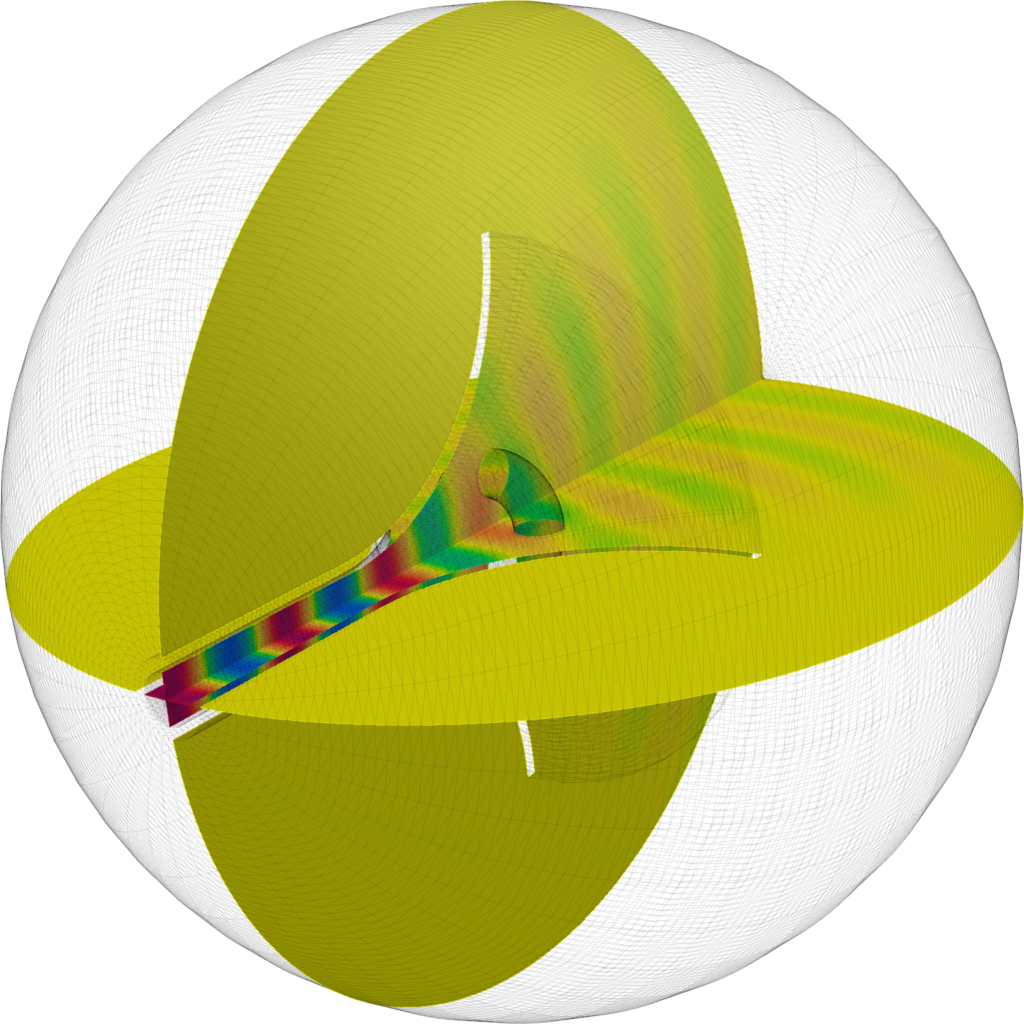
\includegraphics[width=0.35\textwidth]{figs/cover}
\end{center}

\vfill

\section*{Contents}
%
%\begin{center}A BRIEF INTRODUCTION\end{center}
%
\textbf{Tutorial 1.~~~}
The First FreeFEM Example\dotfill~3

\textbf{Tutorial 2.~~~}
Dirichlet Boundary Conditions\dotfill~8

\textbf{Tutorial 3.~~~}
Unstructured Meshes and Domain Indicators\dotfill~12

\textbf{Tutorial 4.~~~}
FE Spaces on Subdaomains and Mesh Truncation\dotfill~21

\textbf{Tutorial 5.~~~}
Additional Mesh-Related Tools\dotfill~28

\textbf{Appendix.~~~}
A Note on PETSc Solvers and Preconditioners\dotfill~32

\vfill

{\footnotesize
Fotios Kasolis~\copyright~Copyright 2020. This work is released under the GNU General Public License, version 3.}

\newpage\thispagestyle{empty}\phantom{.}\newpage\thispagestyle{empty}

\section{\hrulefill\\Tutorial 1. The First FreeFEM Example}
Consider the Poisson equation $-\Delta u = x$ in the unit square $\varOmega = (0,1)\times(0,1)$, together with the homogeneous Dirichlet boundary condition $u=0$ on the bottom and right boundaries $\varGamma_\mathrm{D}$ and the homogeneous Neumann boundary condition $\partial u/\partial n=0$ on the residual part of the boundary. The variational form of this problem reads
\[
\text{<<find $u\in V$ such that }a(u,v)\equiv\int_\varOmega \nabla u \cdot \nabla v = \int_\varOmega x v\equiv\ell(v)\quad\forall v\in V\text{>>},
\]
where $V=\{v\in L^2(\varOmega):\nabla v\in [L^2(\varOmega)]^2\text{ and }v|_{\varGamma_\mathrm{D}}=0\}$. FreeFEM can be used for all steps that are involved in the solution process of this problem with the finite element method (FEM). In particular, FreeFEM can be used for
%
\begin{itemize}
\item generating a triangulation,
\item declaring a finite element space over the generated triangulation, 
\item defining trial and test functions as members of the declared finite element space,
\item specifying, assembling, and solving the linear system.
\end{itemize}
%%%%%%%%%%%%%%%%%%%%%%%%%%%%%%%%%%%%%%%%%%%%%%%%%%%%%%%%%%%%%%%%%%%%%%%%%%%%%%%%

\vspace*{0.2cm}
\textbf{1.1 Generating a structured triangulation}
\begin{Verbatim}[commandchars=\\\{\}]
mesh T = square(10, 10);
cout << "USER/ Number of vertices : " << T.nv   << endl;
cout << "USER/ Number of triangles: " << T.nt   << endl;
cout << "USER/ Minimum edge-length: " << T.hmin << endl;
cout << "USER/ Maximum edge-length: " << T.hmax << endl;
plot(T, wait = true, ps = "mesh.eps");
\dotfill
USER/ Number of vertices : 121
USER/ Number of triangles: 200
USER/ Minimum edge-length: 0.1
USER/ Maximum edge-length: 0.141421

\hfill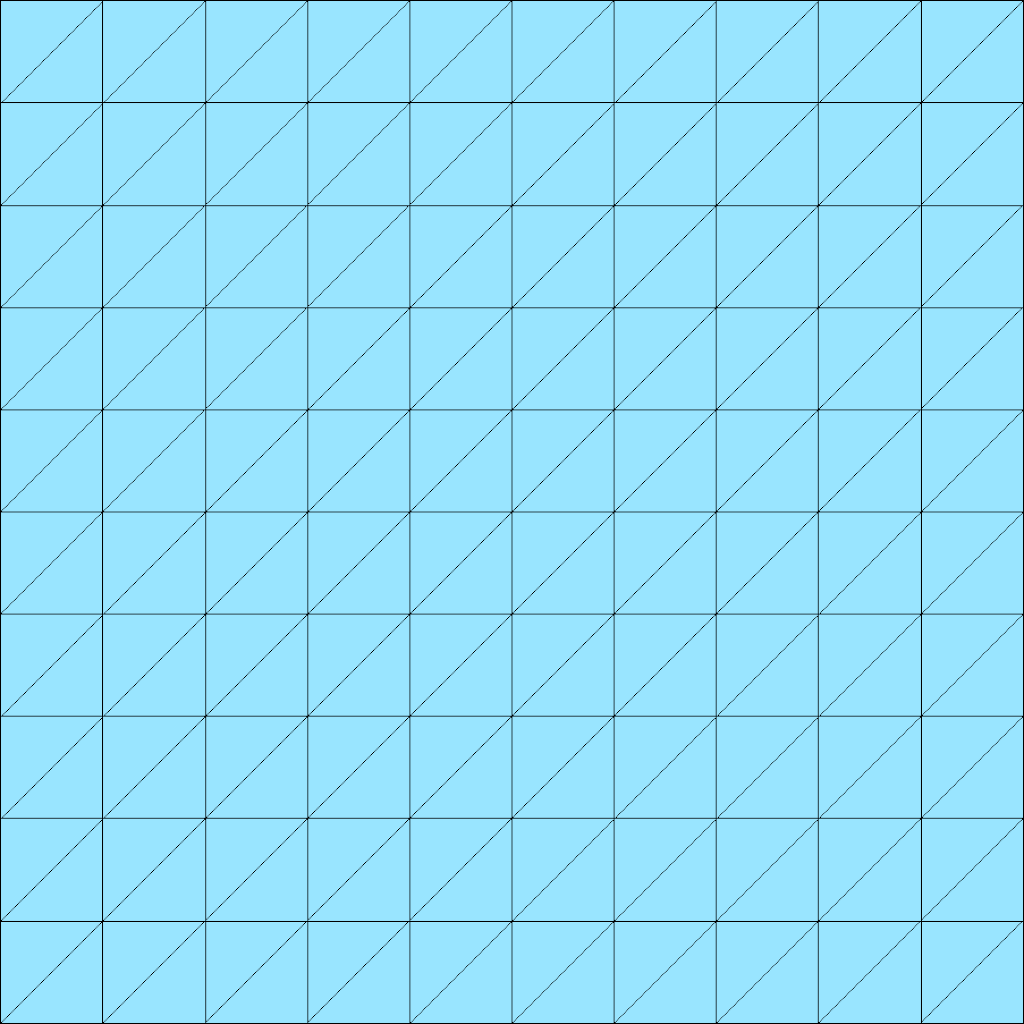
\includegraphics[width=0.45\textwidth]{figs/01}\hfill
\end{Verbatim}

\begin{itemize}
\item Save the FreeFEM instructions in a simple text file, say \verb!xmpl-01.edp!, and execute the script by calling \verb!FreeFem++ xmpl-01.edp! in a terminal.
\item The arguments of \verb!square! specify the number of edges that are used for discretizing the boundary of the unit square in the $x$ and $y$ directions.
\end{itemize}
%%%%%%%%%%%%%%%%%%%%%%%%%%%%%%%%%%%%%%%%%%%%%%%%%%%%%%%%%%%%%%%%%%%%%%%%%%%%%%%%

\vspace*{0.2cm}
\textbf{1.2 Declaring a finite element space}
\begin{Verbatim}[commandchars=\\\{\}]
fespace V(T, P2);
cout << "USER/ Number of degrees of freedom: " << V.ndof << endl;
\dotfill
USER/ Number of degrees of freedom: 441
\end{Verbatim}

\begin{itemize}
\item Here, \verb!P2! instructs FreeFEM to build the finite element space whose basis functions are second-degree polynomials within each triangle.
\item Similarly, \verb!P0! and \verb!P1! can be used for element-wise constant and linear polynomial basis functions, respectively. 
\end{itemize}
%%%%%%%%%%%%%%%%%%%%%%%%%%%%%%%%%%%%%%%%%%%%%%%%%%%%%%%%%%%%%%%%%%%%%%%%%%%%%%%%

\vspace*{0.2cm}
\textbf{1.3 Defining finite element functions}
\begin{Verbatim}[commandchars=\\\{\}]
V u, v;
u = sin(2.0*pi*x)*sin(2.0*pi*y);
cout << "USER/ Number of array components: " << u[].n << endl;
plot(u, value = true, fill = true, wait = true, ps = "fefunc.eps");
\dotfill
USER/ Number of array components: 441

\hfill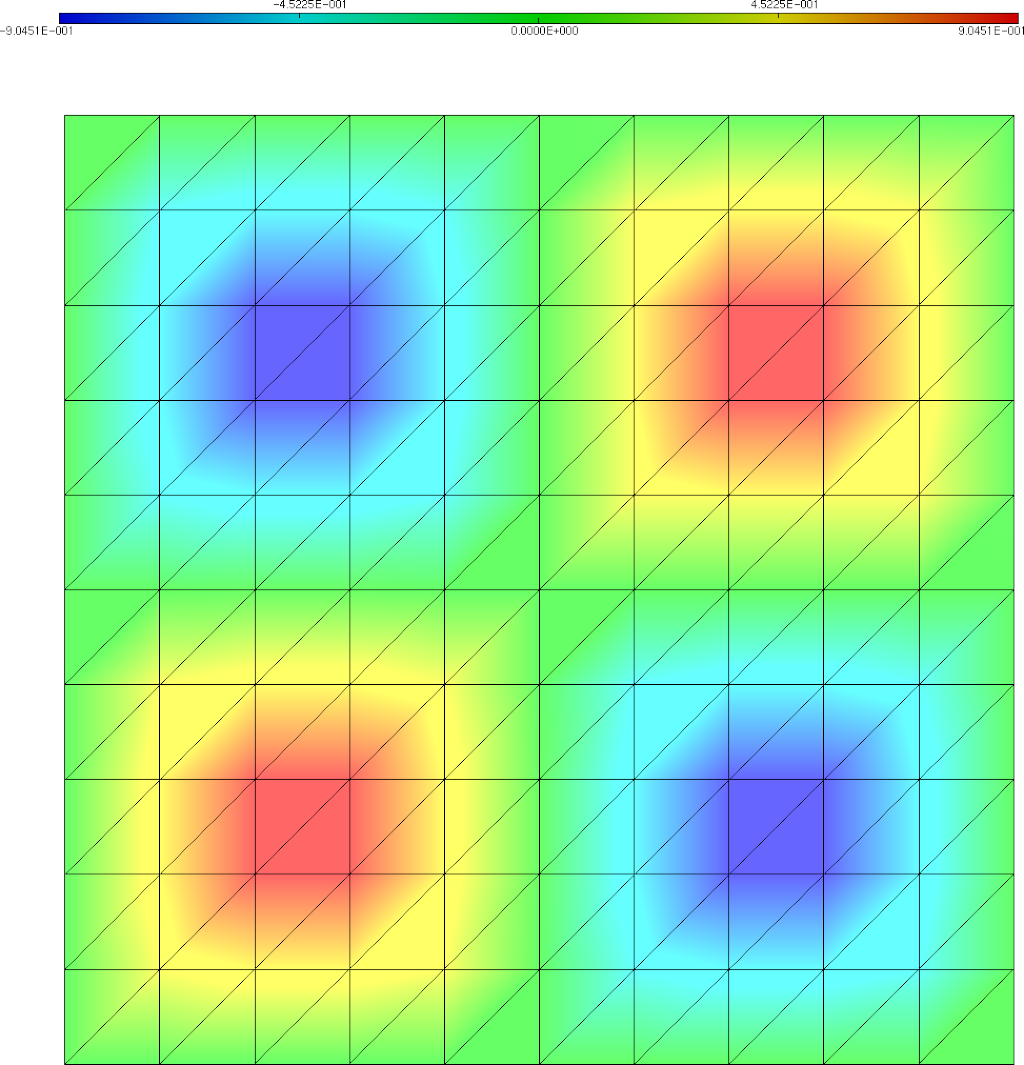
\includegraphics[width=0.45\textwidth]{figs/03}\hfill
\end{Verbatim}

\begin{itemize}
\item The constant $\uppi\approx 3.14$ and the function $\sin$ are known by FreeFEM as \verb!pi! and \verb!sin!, respectively, while \verb!x! and \verb!y! are the reserved space variables. The value of \verb!u! at a point with \verb!x0! and \verb!y0!, can be obtained with the syntax \verb!u(x0,y0)!.
\item If \verb!u! is a finite element function, then \verb!u[]! is the associated \verb!real[int]! array, with indexing starting at zero. Hence, \verb!u[][k]!, with \verb!k=0,1,...,V.ndof-1!, are the values of \verb!u! at the degrees of freedom. 
\item Arrays of type \verb!real[int]! admit the methods \verb!n!, \verb!min!, \verb!imin!, \verb!max!, \verb!imax!, \verb!sum!, \verb!sort!, \verb!l1!, \verb!l2!, \verb!linfty!. In the following example, the \verb!P1! basis function at node index \verb!4!, which is located at the center of the domain, is constructed. 
\end{itemize}

\begin{Verbatim}[commandchars=\\\{\}]
mesh T = square(2, 2);
fespace V(T, P1);
V u = 0.0;
u[][4] = 1.0;
cout << "USER/ max(u)    = " << u[].max  << endl;
cout << "USER/ argmax(u) = " << u[].imax << endl;
plot(u, value = true, fill = true, wait = true, ps = "febasis.eps");
\dotfill
USER/ max(u)    = 1
USER/ argmax(u) = 4

\hfill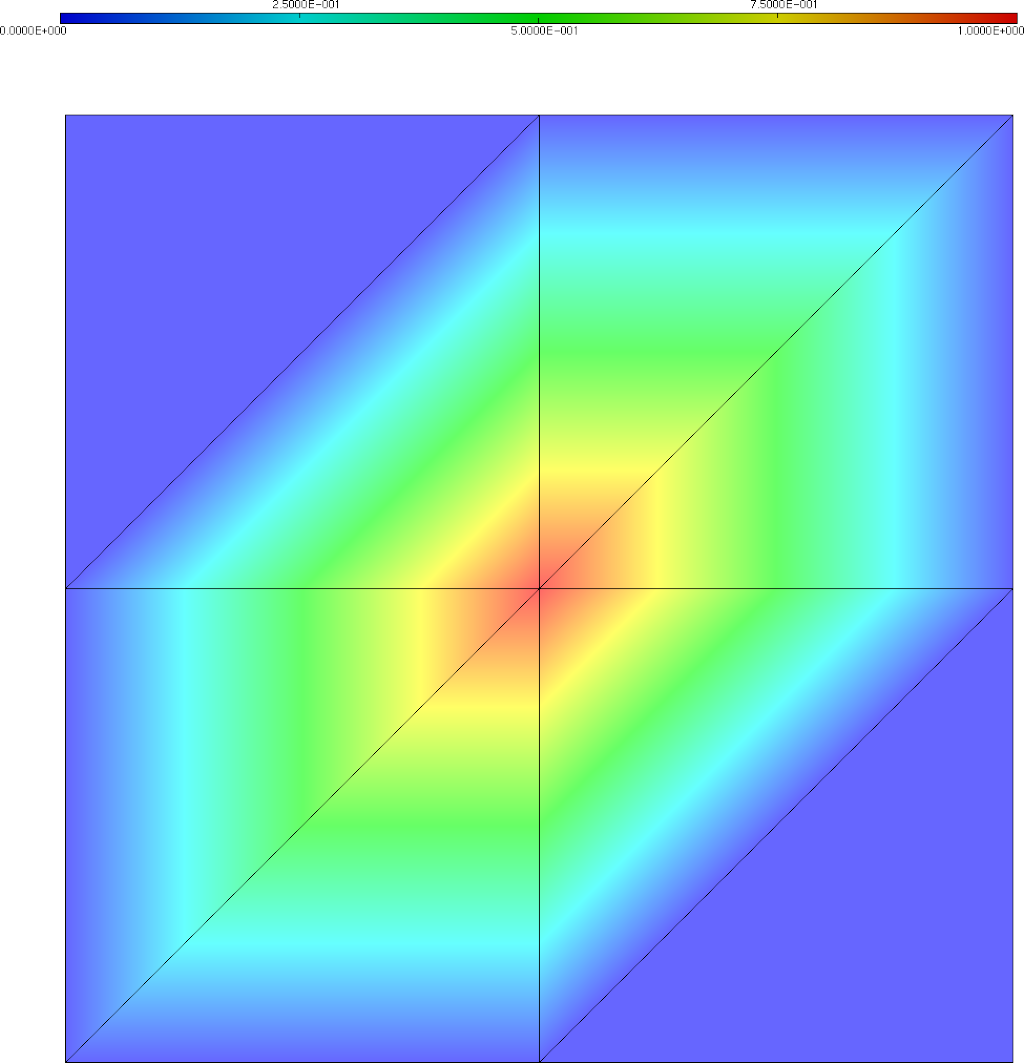
\includegraphics[width=0.45\textwidth]{figs/04}\hfill
\end{Verbatim}
%%%%%%%%%%%%%%%%%%%%%%%%%%%%%%%%%%%%%%%%%%%%%%%%%%%%%%%%%%%%%%%%%%%%%%%%%%%%%%%%

\vspace*{0.2cm}
\textbf{1.4 Defining, assembling, and solving the linear system}
\begin{Verbatim}[commandchars=\\\{\}]
// QUICK SOLUTION METHOD 1: DEFINE AND SOLVE
solve Poisson(u, v)   = int2d(T)( dx(u)*dx(v) + dy(u)*dy(v) )
                        - int2d(T)( x*v ) + on(1, 2, u = 0.0);
                      
// QUICK SOLUTION METHOD 2: DEFINE THEN SOLVE
problem Poisson(u, v) = int2d(T)( dx(u)*dx(v) + dy(u)*dy(v) )
                        - int2d(T)( x*v ) + on(1, 2, u = 0.0);
Poisson; //solve
\end{Verbatim}

\begin{itemize}
\item The sought finite element function variable \verb!u! must appear as the first argument of the problem's tag \verb!Poisson!, while the bilinear and linear forms must be under separate integrals.
\item The functions \verb!dx! and \verb!dy! evaluate the partial derivatives of a finite element function with respect to $x$ and $y$, respectively, and they return finite element functions.
\item The function \verb!on! imposes Dirichlet boundary conditions on the boundaries with labels \verb!1! and \verb!2!. The function \verb!square! returns the labels \verb!1!, \verb!2!, \verb!3!, \verb!4! for the bottom, right, top, and left boundaries, respectively.
\item To separate the assembly from the solution process, and hence, gain control at the level of linear algebra, \verb!varf! can be used to separately define the bilinear form and the linear form, as in the example below.
\end{itemize}

\begin{Verbatim}[commandchars=\\\{\}]
// PREFERRED SOLUTION METHOD
varf a(u, v) = int2d(T)( dx(u)*dx(v) + dy(u)*dy(v) ) 
               + on(1, 2, u = 0.0);
varf l(u, v) = int2d(T)( x*v ) + on(1, 2, u = 0.0);
matrix A = a(V, V);    // assemble bilinear form
real[int] b = l(0, V); // assemble linear form
u[] = A^-1*b;          // solve
plot(u, value = true, fill = true, wait = true, ps = "solution.eps");
\dotfill

\hfill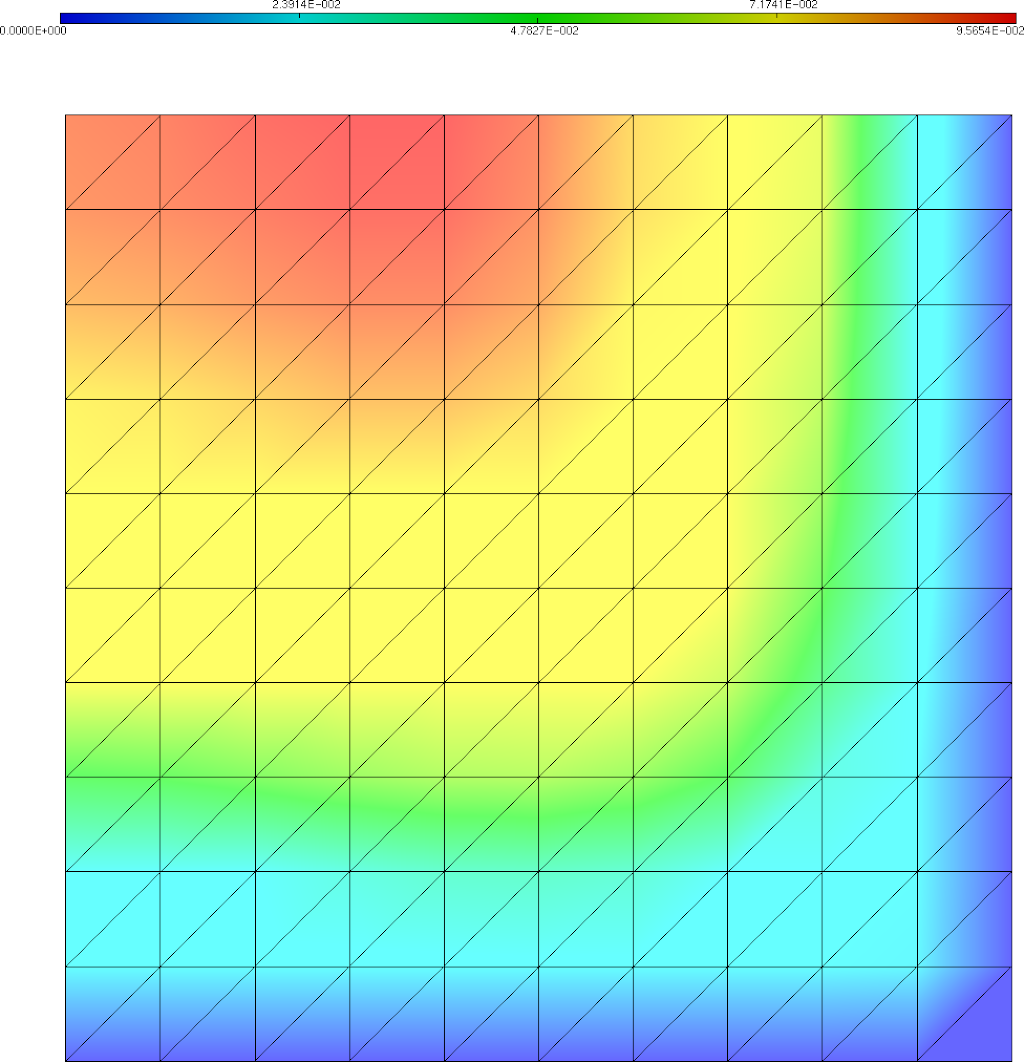
\includegraphics[width=0.45\textwidth]{figs/05}\hfill
\end{Verbatim}

\begin{itemize}
\item The finite element functions \verb!u!, \verb!v!  do not have to be defined before the \verb!varf! statement; in particular, the test function \verb!v! does not need to be defined at all. The first argument of the linear form is not used.
\item Dirichlet boundary data must be imposed to the bilinear form and to the linear form, although the actual value imposed on the bilinear form has no effect.
\item The bilinear form needs to be assembled as a \verb!matrix! sparse matrix, while the linear form as a \verb!real[int]! array.
\item The complete code for solving the problem of this tutorial follows.
\end{itemize}

\begin{Verbatim}[commandchars=\\\{\}]
mesh T = square(10, 10);
fespace V(T, P2);
varf a(u, v) = int2d(T)( dx(u)*dx(v) + dy(u)*dy(v) ) 
               + on(1, 2, u = 0.0);
varf l(u, v) = int2d(T)( x*v ) + on(1, 2, u = 0.0);
matrix A = a(V, V);
real[int] b = l(0, V);
V u;
u[] = A^-1*b; //return solution as real[int] array
plot(u, fill = true, wait = true);
\end{Verbatim}
%%%%%%%%%%%%%%%%%%%%%%%%%%%%%%%%%%%%%%%%%%%%%%%%%%%%%%%%%%%%%%%%%%%%%%%%%%%%%%%%

\vspace*{0.2cm}
\textbf{1.5 Solving the same problem with $\varOmega$ being the unit cube}
\begin{Verbatim}[commandchars=\\\{\}]
load "msh3" //import three-dimensional meshing tools
mesh3 T = cube(10, 10, 10);
fespace V(T, P1);
varf a(u, v) = int3d(T)( dx(u)*dx(v) + dy(u)*dy(v) + dz(u)*dz(v) )
               + on(1, 2, u = 0.0);
varf l(u, v) = int3d(T)( x*v ) + on(1, 2, u = 0.0);
matrix A = a(V, V);
real[int] b = l(0, V);
V u;
u[] = A^-1*b;
plot(u, value = true, fill = true, nbiso = 64, wait = true);
\dotfill

\hfill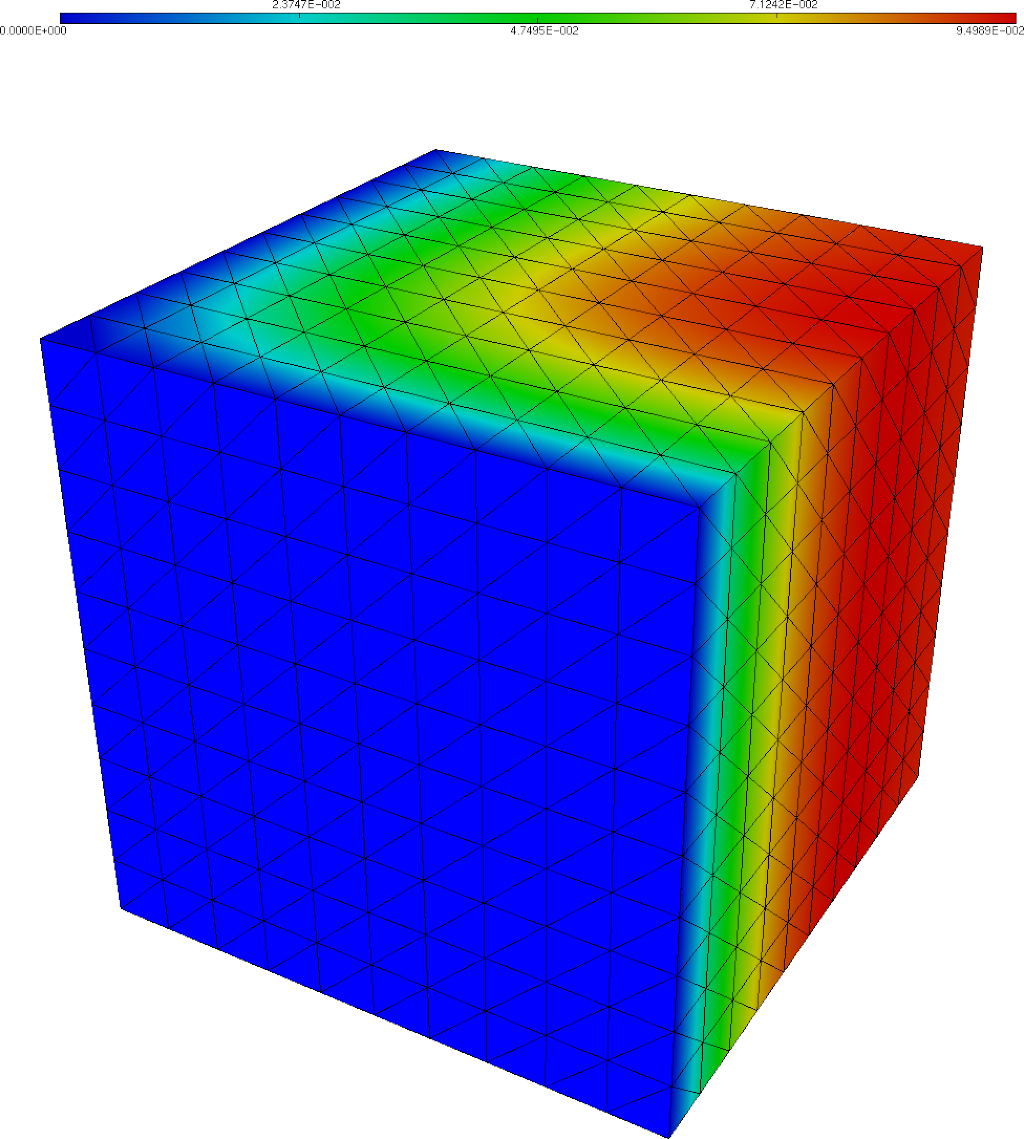
\includegraphics[width=0.45\textwidth]{figs/07}\hfill
\end{Verbatim}

\begin{itemize}
\item After importing the three-dimensional meshing tools with \verb!load "msh3"!, FreeFEM requires a minimal modification of the two-dimensional problem. In particular, \verb!mesh! becomes \verb!mesh3!, \verb!square! becomes \verb!cube!, \verb!int2d! becomes \verb!int3d!, while in $\mathbb{R}^3$, the scalar product of the gradients has the additional term \verb!dz(u)*dz(v)!.
\item In \verb!plot!, the additional option \verb!nbiso=64! specifies the number of isosurfaces to be used.
\end{itemize}
%%%%%%%%%%%%%%%%%%%%%%%%%%%%%%%%%%%%%%%%%%%%%%%%%%%%%%%%%%%%%%%%%%%%%%%%%%%%%%%%

\vspace*{0.2cm}
\textbf{1.6 Parallelizing with domain decomposition}

\begin{Verbatim}[commandchars=\\\{\}]
// EXECUTION: mpiexec -n 8 FreeFem++-mpi xmpl-03.edp -wg
load "PETSc"                // PETSc plugin
macro dimension() 3         // three-dimensional problem
include "macro_ddm.idp"     // additional definitions

mesh3 T = cube(10, 10, 10); // global mesh
Mat A;
createMat(T, A, P2);

// AFTER THIS POINT FESPACES AND FUNCTIONS ARE LOCAL TO THE PORCESS
fespace V(T, P2);
varf a(u, v) = int3d(T)( dx(u)*dx(v) + dy(u)*dy(v) + dz(u)*dz(v) )
               + on(1, 2, u = 0.0);
varf l(u, v) = int3d(T)( x*v ) + on(1, 2, u = 0.0);
A = a(V, V, tgv = -1);
real[int] b = l(0, V, tgv = -1);
V u;
u[] = A^-1 * b;

// PLOT GLOBAL SOLUTION
macro def(u) u//
plotMPI(T, u, P2, def, real, cmm = "Solution");
\end{Verbatim}
\begin{itemize}
\item After importing PETSc, defining the dimension of the problem as a \verb!macro!, and importing domain decomposition tools, minimal modifications are needed. In particular, the bilinear form is assembled as a PETSc matrix \verb!Mat! and is distributed using \verb!createdMat!.
\item To plot the global solution, \verb!plotMPI! is used, instead of \verb!plot!. Here, the function \verb!plotMPI! constructs \verb!real! local finite element spaces of type \verb!P2! on the subdomains of \verb!T!. The \verb!def! macro informs \verb!plotMPI! that the solution is a scalar function.
\end{itemize}

\section{\hrulefill\\Tutorial 2. Dirichlet Boundary Conditions}
Here, the problem of interest is the Poisson equation $\Delta u = 1$ in the unit square, but with a non-homogeneous Dirichlet boundary condition on $\varGamma_\mathrm{D}=\{\verb!2!,\verb!4!\}$, say $u=u_\mathrm{D}\neq 0$, and a homogeneous Neumann boundary condition on the residual part of the boundary. The variational form of this problem reads
\[
\text{<<find $u\in V_{u_\mathrm{D}}$ such that }a(u,v)=\int_\varOmega v\equiv\ell(v)\quad\forall v\in V_0\text{>>},
\]
where $V_\ast=\{v\in L^2(\varOmega):\nabla v\in [L^2(\varOmega)]^2\text{ and }v|_{\varGamma_\mathrm{D}}=\ast\}$. To impose this Dirichlet condition, \verb!on(2, 4, u = uD)! has to be used in the \verb!varf! definitions of $a$ and $\ell$. The default implementation of the \verb!on! function employs the following penalization method. If the $i$-th degree of freedom has one of the labels that are given to \verb!on!, then the corresponding diagonal entry $a_{ii}$ of the matrix $\bm{A}$ that is assembled from the bilinear form is set to $1/\epsilon\gg 1$, while the corresponding component $b_i$ of the right-hand side vector $\bm{b}$ becomes $u_\mathrm{D}(x_i,y_i)/\epsilon$. Then, the equation that is associated with the $i$-th (Dirichlet constraint) degree of freedom is
\[
a_{i1} u_1 + \cdots + u_i/\epsilon + \cdots + a_{iN} u_N = u_\mathrm{D}(x_i,y_i)/\epsilon,
\]
and since the term $u_i/\epsilon$ dominates the left-hand side sum, the solution at the $i$-th degree of freedom becomes $u_i\approx u_\mathrm{D}(x_i,y_i)$. FreeFEM provides two alternatives, while assembling $\bm{A}$ and $\bm{b}$, throught the option \verb!tgv!. Currently, if \verb!tgv! is set to \verb!-1! (subject to change, \verb!-10! in future releases), then all non-diagonal entries of the $i$-th row of $\bm{A}$ are set to zero, while $a_{ii}=1$. Thus, setting \verb!tgv=1.0! when assembling the right-hand side results in $u_i=u_\mathrm{D}(x_i,y_i)$ and the boundary condition is set exactly. Both the default penalty approach and the \verb!tgv=-1! row-wise elimination method are subject to certain disadvantages, when iterative solvers are to be used for solving $\bm{Au}=\bm{b}$. For instance, row-wise elimination breaks the symmetry of $\bm{A}$. The last option that is offered by FreeFEM is the row/column-wise elimination, which is selected by setting \verb!tgv! to \verb!-2! (subject to change, \verb!-20! in future releases). Unfortunately, the row/column-wise elimination method requires an additive modification of the right-hand side, unless the solution is vanishing on the Dirichlet boundary. Such a modification is not automated in FreeFEM, but is trivial to implement, as shown below.
%%%%%%%%%%%%%%%%%%%%%%%%%%%%%%%%%%%%%%%%%%%%%%%%%%%%%%%%%%%%%%%%%%%%%%%%%%%%%%%%

\vspace*{0.2cm}
\textbf{2.1 Homogenizing Dirichlet data in the variational setting}\\
Here, the variational problem itself is modified so that the Dirichlet boundary condition becomes homogeneous. In this scenario, the boundary data appear as a volume source in the linear form of the variational problem. In particular, assume that $u$ admits a decomposition of the form $u=u_0+\mathcal{E}u_\mathrm{D}$, where $\mathcal{E}u_\mathrm{D}$ is an extension of the Dirichlet data into $\varOmega$. Since $\mathcal{E}u_\mathrm{D}|_{\varGamma_\mathrm{D}}=u_\mathrm{D}$ and $u|_{\Gamma_\mathrm{D}}=u_\mathrm{D}$, it follows that $u_0|_{\varGamma_\mathrm{D}}=0$. This modification results in the variational problem
\[
\text{<<find $u_0\in V_0$ such that }\int_{\varOmega}\nabla u_0 \cdot\nabla v = \int_{\varOmega} v - \int_{\varOmega}\nabla \mathcal{E}u_\mathrm{D}\ \cdot\nabla v\quad\forall v\in V_0\text{>>}.
\]
Then, row/column-wise elimination can be used for $\bm{A}$, without modifying the right-hand side vector $\bm{b}$, since the additive contribution of the Dirichlet constraint degrees of freedom is vanishing. In the following example, $u_\mathrm{D}=y$ and an extension $\mathcal{E}u_\mathrm{D}$ that vanishes a strip away from the Dirichlet boundary is implemented.

\begin{Verbatim}[commandchars=\\\{\}]
mesh T = square(10, 10);
fespace V(T, P2);

// EXTENSION OF DIRICHLET DATA
varf bndDirichlet(u, v) = on(2, 4, u = y);
V EuD;
EuD[] = bndDirichlet(0, V, tgv = 1.0);
plot(EuD, value = true, fill = true, wait = true);

// DEFINITION OF FORMS, ASSEMBLY, AND SOLUTION
varf a(u, v) = int2d(T)( dx(u)*dx(v) + dy(u)*dy(v) ) 
               + on(2, 4, u = 0.0);
varf l(u, v) = int2d(T)( v - dx(EuD)*dx(v) - dy(EuD)*dy(v) ) 
               + on(2, 4, u = 0.0);
matrix A = a(V, V, tgv = -2);
real[int] b = l(0, V);
V u0;
u0[] = A^-1*b;
plot(u0, value = true, fill = true, wait = true, cmm = "u0");

// COMPUTATION OF SOLUTION TO THE ORIGINAL PROBLEM
V u = u0 + EuD;
plot(u, value = true, fill = true, wait = true, cmm = "u");

// DEFAULT DIRICHLET DATA IMPLEMENTATION
V uDef, v;
solve varDef(uDef, v) = int2d(T)( dx(uDef)*dx(v) + dy(uDef)*dy(v) )
                        - int2d(T)( v ) + on(2, 4, uDef = y);
plot(uDef, value = true, fill = true, wait = true, cmm = "Default u");

// DIFFERENCE BETWEEN HOMOGENIZED AND DEFAULT D.DATA IMPLEMENTATION
V diff = abs(u - uDef);
plot(diff, value = true, fill = true, wait = true, cmm = "Difference");
\dotfill

\hfill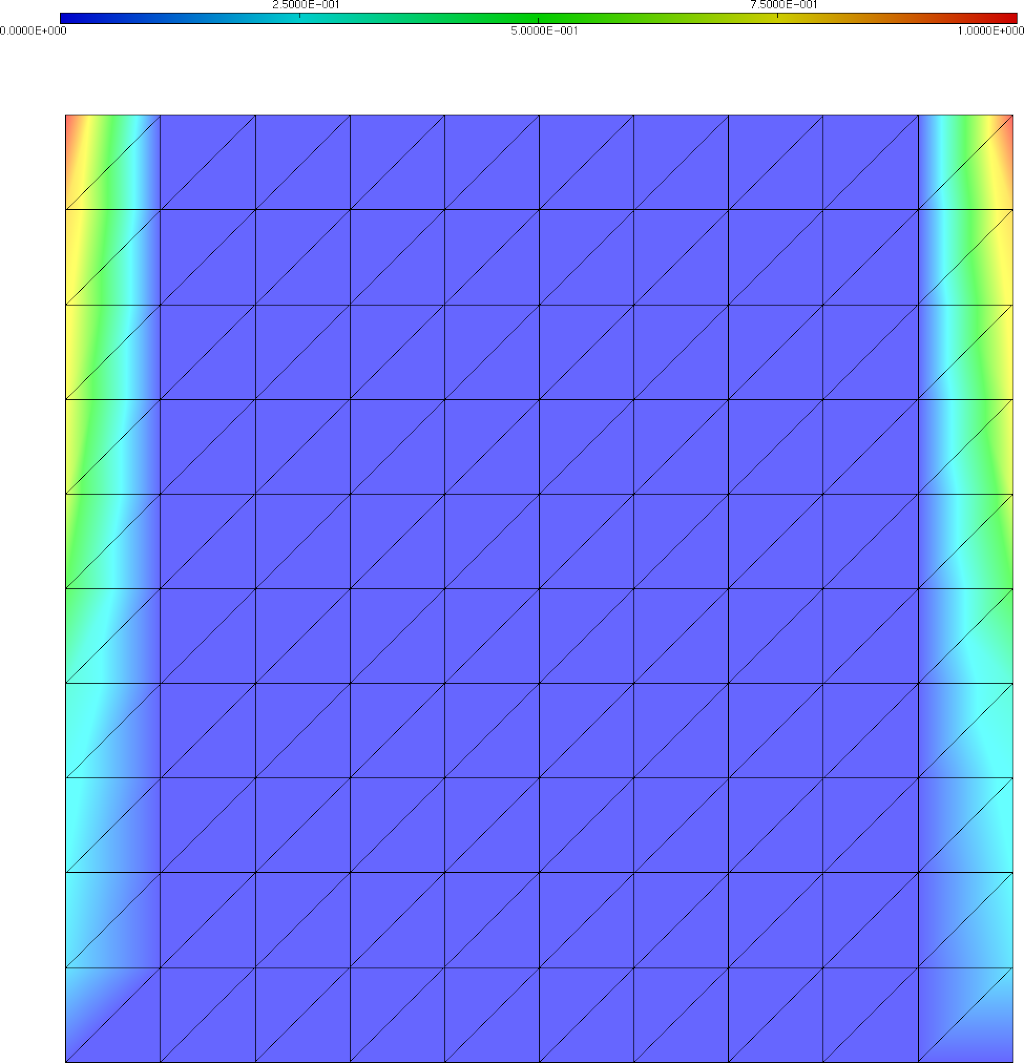
\includegraphics[width=0.45\textwidth]{figs/08}\hfill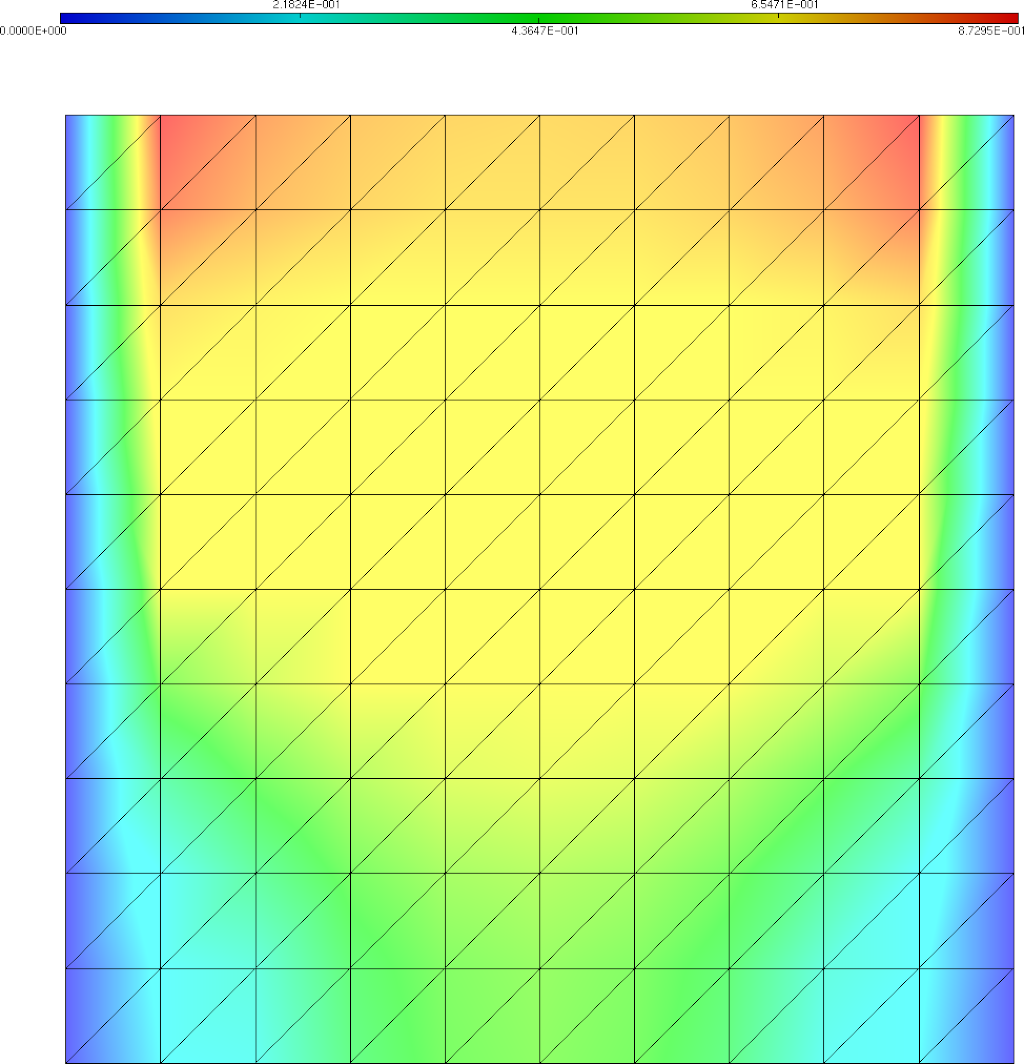
\includegraphics[width=0.45\textwidth]{figs/09}\hfill

\hfill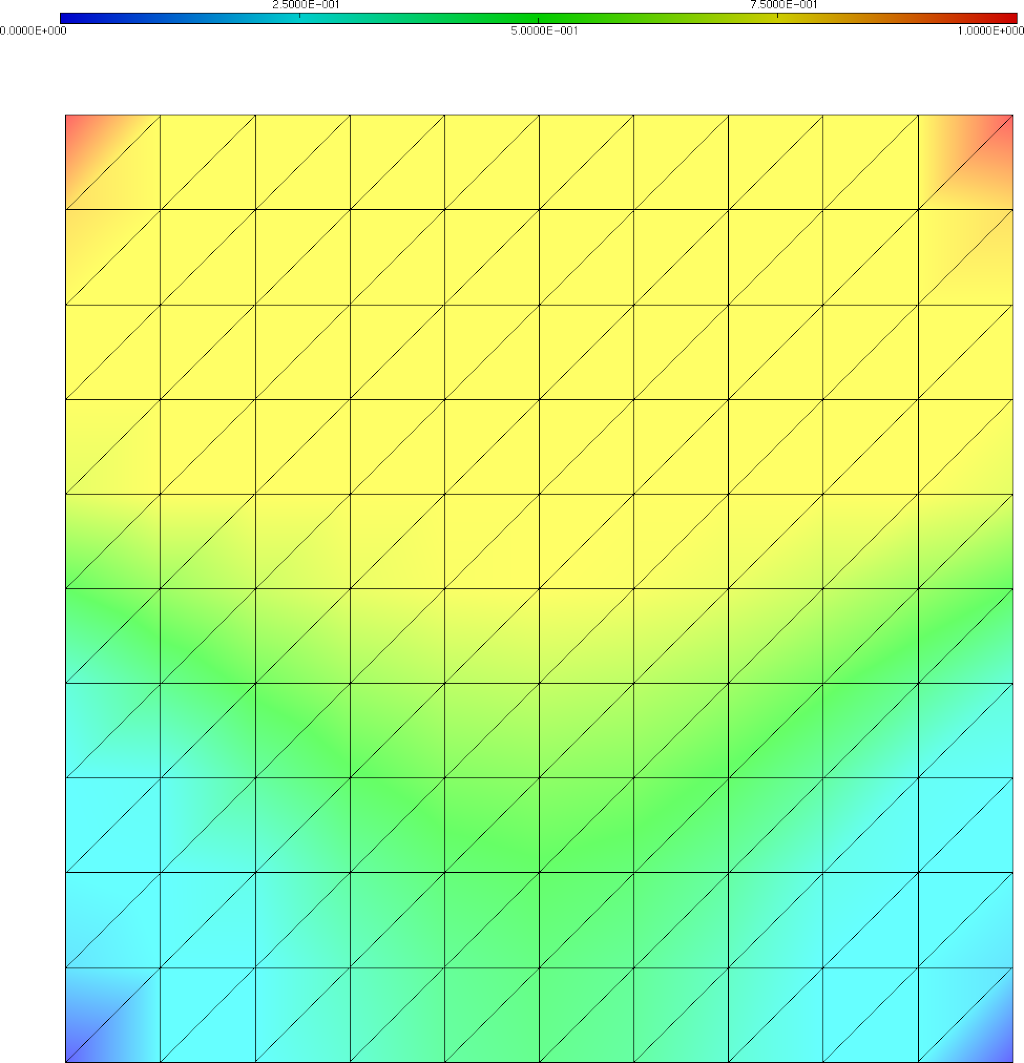
\includegraphics[width=0.45\textwidth]{figs/10}\hfill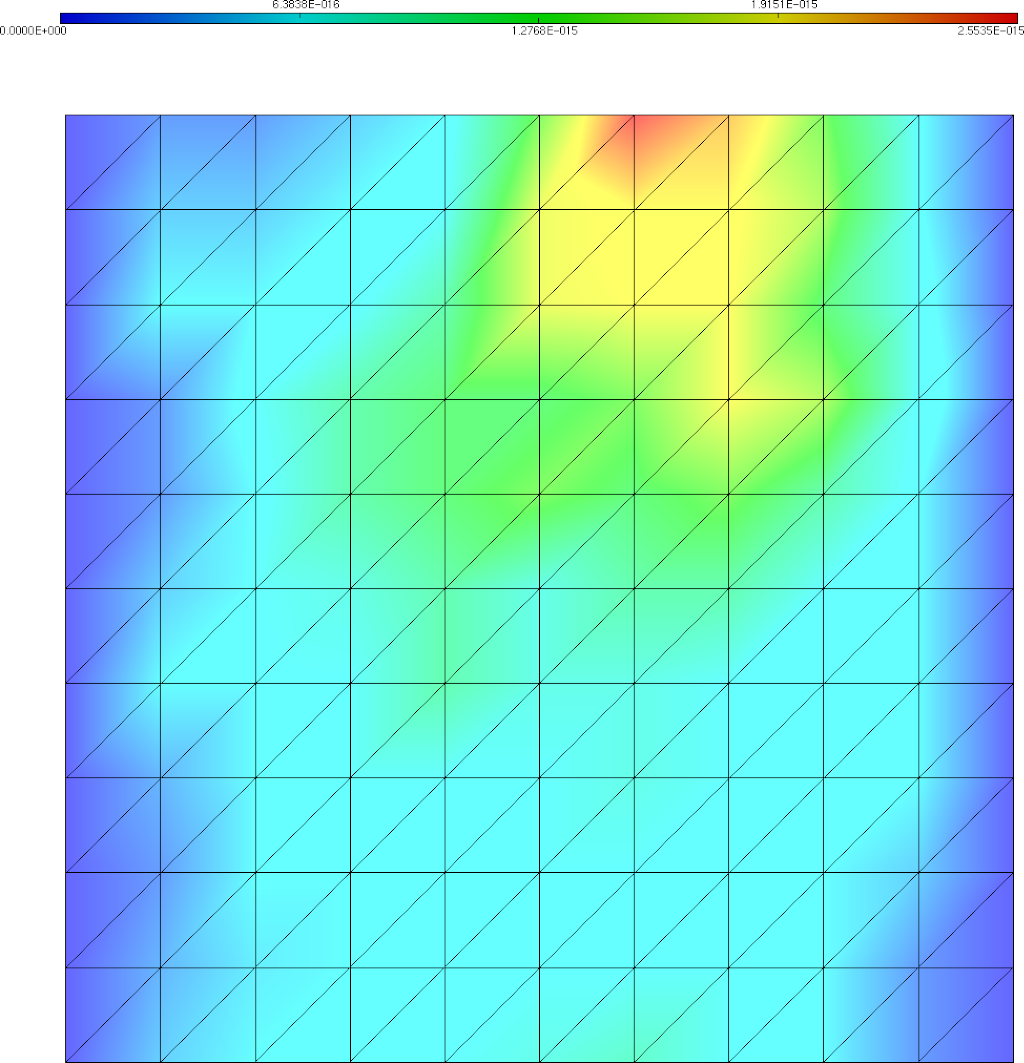
\includegraphics[width=0.45\textwidth]{figs/11}\hfill
\end{Verbatim}

\begin{itemize}
\item The \verb!varf! object \verb!bndDirichlet! defines the extension $\mathcal{E}y$ in the \verb!P2! space \verb!V!. When assembling the \verb!real[int]! array \verb!EuD[]!, the option \verb!tgv=1.0! sets $1/\epsilon=1.0$, while the same result can be achieved with \verb!tgv=-1! and \verb!tgv=-2! for such arrays.
\item In the \verb!varf! definition of the bilinear form \verb!a!, the \verb!on! function is used for informing FreeFEM which rows and columns of \verb!A! are Dirichlet constrained, while the value that is prescribed to \verb!u! has no effect.
\end{itemize}
%%%%%%%%%%%%%%%%%%%%%%%%%%%%%%%%%%%%%%%%%%%%%%%%%%%%%%%%%%%%%%%%%%%%%%%%%%%%%%%%

\vspace*{0.2cm}
\textbf{2.2 Homogenizing Dirichlet data in the linear algebra setting}\\
Having in mind the variational-to-linear algebra mappings $a(u,\ast)\leftarrow\bm{Au}$ and $\ell(\ast)\leftarrow\bm{b}$, it can be seen that the equation of the variational problem with homogenized Dirichlet data can be written
\[
\bm{Au}=\bm{b}_1 - \bm{b}_2,
\]
where $\bm{b}_1$ is the vector that is associated with the first term of the right-hand side, which actually is the right-hand side of the original problem, and $\bm{b}_2=\bm{A}\mathcal{E}\bm{u}_\mathrm{D}$ is associated with the volume source that arises due to the homogenization of the Dirichlet data.

\begin{Verbatim}[commandchars=\\\{\}]
mesh T = square(10, 10);
fespace V(T, P2);

// EXTENSION OF DIRICHLET DATA
varf bndDirichlet(u, v) = on(2, 4, u = y);
V EuD;
EuD[] = bndDirichlet(0, V, tgv = 1.0);

// DEFINITION OF FORMS, ASSEMBLY, AND SOLUTION
varf a(u, v) = int2d(T)( dx(u)*dx(v) + dy(u)*dy(v) )
               + on(2, 4, u = 0.0);
varf l(u, v) = int2d(T)( v )
               + on(2, 4, u = 0.0);

matrix A = a(V, V, tgv = -1); // is not symmetric
real[int] b1 = l(0, V);       // zeros at boundary components
real[int] b2 = A*EuD[];       // EuD   at boundary components
real[int] b = b1 - b2;        //-EuD   at boundary components
b = b + EuD[];                // zeros at boundary components

A = a(V, V, tgv = -2);        // is symmetric
V u0;
u0[] = A^-1*b;

// COMPUTATION OF SOLUTION TO THE ORIGINAL PROBLEM
V u = u0 + EuD;
plot(u, value = true, fill = true, wait = true, cmm = "u");
\end{Verbatim}

\begin{itemize}
\item Although this implementation comes at the cost of an additional matrix assembly, the user needs to specify the forms of the original problem, and hence, it is easy to black-box it as a \verb!macro!. The following definition can be saved in an \verb!.idp! file, say \verb!ffedd.idp!, and can be called from the main \verb!.edp! file, after being included with \verb!include "ffedd.idp"!.
\end{itemize}

\begin{Verbatim}
// EXACT DIRICHLET DATA SOLVER - FILENAME: ffedd.idp
macro exactDirichletData(oEDDsol, iEDDfespace, iEDDbilinear,
                                               iEDDlinear, iEDDbnd)
{
  matrix A = iEDDbilinear(iEDDfespace, iEDDfespace, tgv = -1);
  real[int] btmp = A*iEDDbnd[];
  real[int] b = iEDDlinear(0, iEDDfespace);
  b -= btmp;
  b += iEDDbnd[];
  A = iEDDbilinear(iEDDfespace, iEDDfespace, tgv = -2);
  iEDDfespace u0;
  u0[] = A^-1*b;
  u = u0 + iEDDbnd;
}//
-----------------------------------------------------------------------
// FILENAME: xmpl-06.edp
include "ffedd.idp"

mesh T = square(10, 10);
fespace V(T, P2);

// EXTENSION OF DIRICHLET DATA
varf bndDirichlet(u, v) = on(2, 4, u = y);
V EuD;
EuD[] = bndDirichlet(0, V, tgv = 1.0);

// DEFINITION OF FORMS
varf a(u, v) = int2d(T)( dx(u)*dx(v) + dy(u)*dy(v) )
               + on(2, 4, u = 0.0);
varf l(u, v) = int2d(T)( v ) + on(2, 4, u = 0.0);

// CALL THE MACRO DEFINED IN ffedd.idp
V u; // global variable space
exactDirichletData(u, V, a, l, EuD);
plot(u, value = true, fill = true, wait = true, cmm = "u");
\end{Verbatim}
\begin{itemize}
\item A macro definition has to end with the comment characters \verb!//!.
\item A \verb!macro! does not distinguish between input and output and has no return values. Here, the following convention is used; the unique output variable is placed first and its identifier starts with \verb!o!, while the input variables follow and their identifiers start with \verb!i!.
\item Since all variables that are defined within a macro are local, to access the solution, the output variable \verb!u! needs to be defined in the global variable space.
\end{itemize}
%%%%%%%%%%%%%%%%%%%%%%%%%%%%%%%%%%%%%%%%%%%%%%%%%%%%%%%%%%%%%%%%%%%%%%%%%%%%%%%%

\section{\hrulefill\\Tutorial 3. Unstructured Meshes and Domain Indicators}
Consider a capacitor with its upper terminal being at constant potential $u_0=1~\mathrm{V}$ and the lower one being grounded. A spherical object of radius $r=0.1~\mathrm{m}$ and relative permittivity $\epsilon_\mathrm{r}=9$ is hanging from the upper plate (with a thread of negligible thickness and relative permittivity close to unity), and is located at the center of the domain, as depicted in the figure below. To perform two-dimensional simulations, the physical domain is truncated; the resulting domain is depicted in the figure below. There, thick lines represent perfect electric insulation, while thinner ones represent perfect electric conductors. Due to the symmetry of the domain with respect to the vertical dashed axis, the computational domain is restricted to the right half plane, namely, $\varOmega$. In the electrostatic scenario, the boundary value problem of interest is 
\[
\nabla\cdot\epsilon\nabla u =0\text{ in }\varOmega,\quad u|_{\varGamma_\mathrm{U}} = 1,\quad
u|_{\varGamma_\mathrm{L}} = 0,\quad\left.\frac{\partial u}{\partial n}\right|_{\varGamma_\mathrm{S}\cup\varGamma_\mathrm{I}} = 0,
\]
where $\varGamma_\mathrm{U}$, $\varGamma_\mathrm{L}$, $\varGamma_\mathrm{S}$, and $\varGamma_\mathrm{I}$ are the upper terminal, the lower terminal, the symmetry, and the insulating boundaries, respectively. The associated variational problem is 
\[
\text{<<find $u\in V_1$ such that }\int_\varOmega \epsilon\nabla u\cdot \nabla v=0\quad\forall v\in V_0\text{>>},
\]
where $V_\ast=\{v\in L^2(\varOmega):\nabla v\in [L^2(\varOmega)]^2\text,~v|_{\varGamma_\mathrm{U}}=\ast,\text{ and }v|_{\varGamma_\mathrm{L}}=0\}$. For simplicity, planar symmetry is assumed.\\
%
\begin{center}
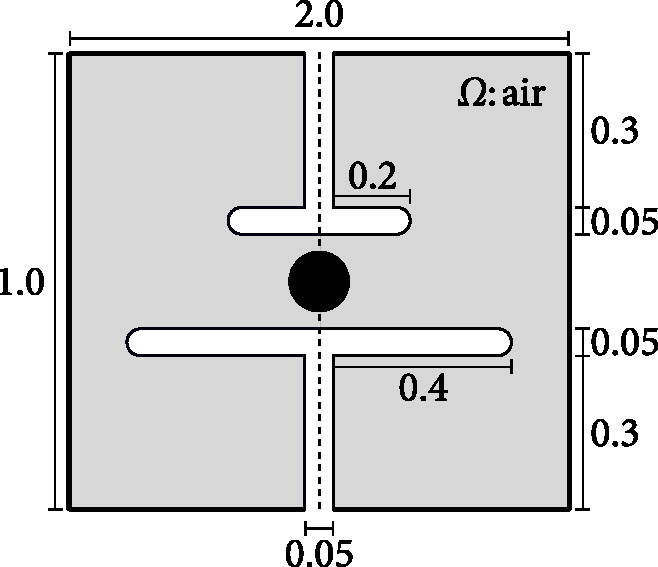
\includegraphics[width=0.45\textwidth]{figs/12}
\end{center}
%
In addition to what has been shown before, here, FreeFEM is used for
%
\begin{itemize}
\item specifying the geometry,
\item generating a triangulation,
\item extracting and modifying domain indicators of distinct regions,
\item defining the permittivity function throughout $\varOmega$,
\item computing the electric field $\bm{E}=-\nabla u$.
\end{itemize}
%%%%%%%%%%%%%%%%%%%%%%%%%%%%%%%%%%%%%%%%%%%%%%%%%%%%%%%%%%%%%%%%%%%%%%%%%%%%%%%%

\vspace*{0.2cm}
\textbf{3.1 Specifying the geometry and generating a triangulation}
\begin{Verbatim}[commandchars=\\\{\}]
// INSULATING BOUNDARIES
border a001(t = 0.025, 1.000)\{x = t    ; y = 0.000  ; label = 0;\}
border a002(t = 0.000, 1.000)\{x = 1.000; y = t      ; label = 0;\}
border a003(t = 1.000, 0.025)\{x = t    ; y = 1.000  ; label = 0;\}

// UPPER TERMINAL BOUNDARIES
border a004(t = 1.000, 0.700)\{x = 0.025; y = t      ; label = 1;\}
border a005(t = 0.025, 0.225)\{x = t    ; y = 0.700  ; label = 1;\}
border a006(t = pi/2 , -pi/2)\{
  x = 0.225 + 0.025*cos(t); y = 0.675 + 0.025*sin(t); label = 1;\}
border a007(t = 0.225, 0.000)\{x = t    ; y = 0.650  ; label = 1;\}

// SYMMETRY CUT BOUNDARIES
border a008(t = 0.650, 0.620)\{x = 0.000; y = t      ; label = 0;\}
border a009(t = 0.620, 0.420)\{x = 0.000; y = t      ; label = 0;\}
border a010(t = 0.420, 0.390)\{x = 0.000; y = t      ; label = 0;\}

// LOWER TERMINAL BOUNDARIES
border a011(t = 0.000, 0.400)\{x = t    ; y = 0.390  ; label = 2;\}
border a012(t = pi/2 , -pi/2)\{
  x = 0.400 + 0.025*cos(t); y = 0.365 + 0.025*sin(t); label = 2;\}
border a013(t = 0.400, 0.025)\{x = t    ; y = 0.340  ; label = 2;\}
border a014(t = 0.340, 0.000)\{x = 0.025; y = t      ; label = 2;\}

// INTERIOR OBJECT BOUNDARY
border a015(t = pi/2 , -pi/2)\{
  x = 0.000 + 0.100*cos(t); y = 0.520 + 0.100*sin(t);           \}

// ARTIFICIAL BORDER FOR NAIVE MESH RESOLUTION CONTROL
border a016(t = 0.620, 0.420)\{x = 0.400; y = t      ;           \}

// GENERATE TRIANGULATION
int n = 20; // integer data type
mesh T = buildmesh(a001(n)   + a002(n)   + a003(n)   +
                   a004(n)   + a005(n)   + a006(n/2) + a007(2*n) +
                   a008(n/2) + a009(2*n) + a010(n/2) +
                   a011(2*n) + a012(n/2) + a013(n)   + a014(n)   +
                   a015(2*n)); // add a016(n)
plot(T, fill = true, wait = true);
\dotfill

\hfill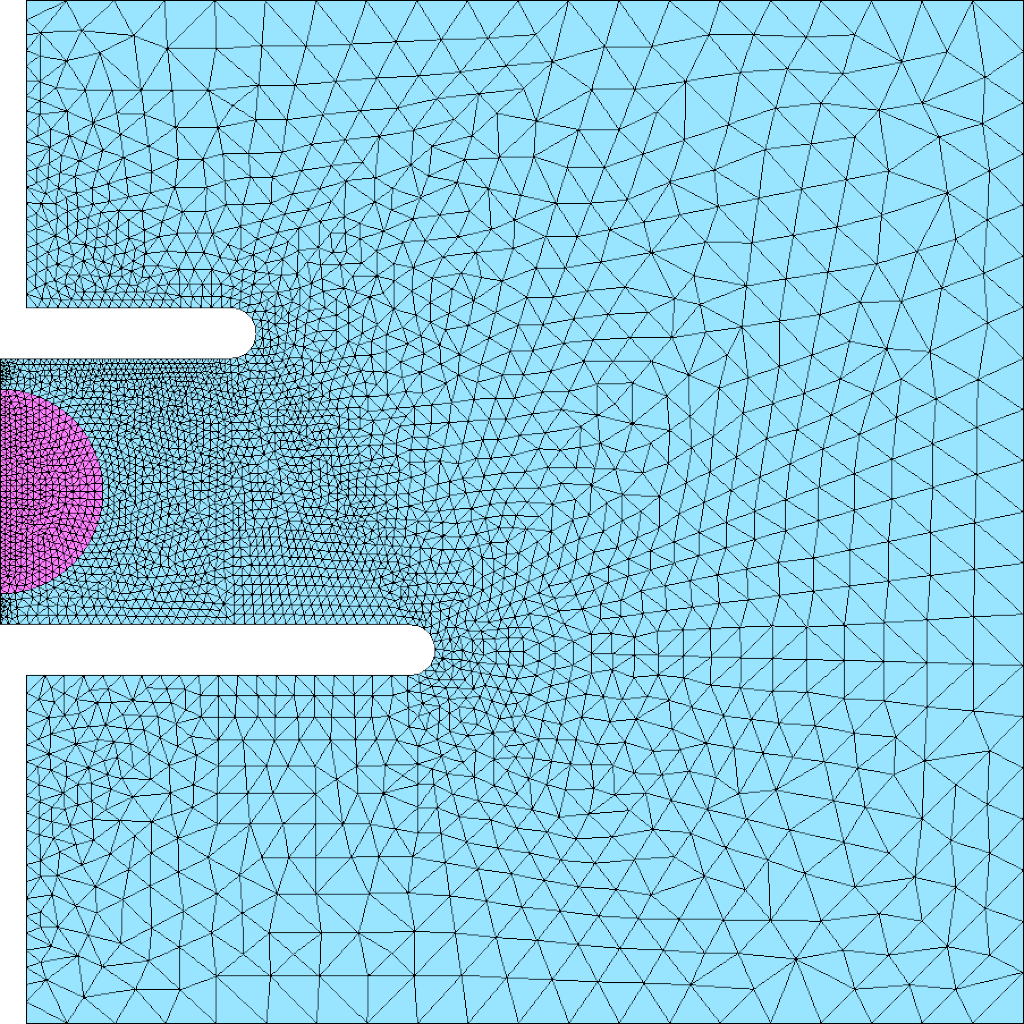
\includegraphics[width=0.45\textwidth]{figs/13}\hfill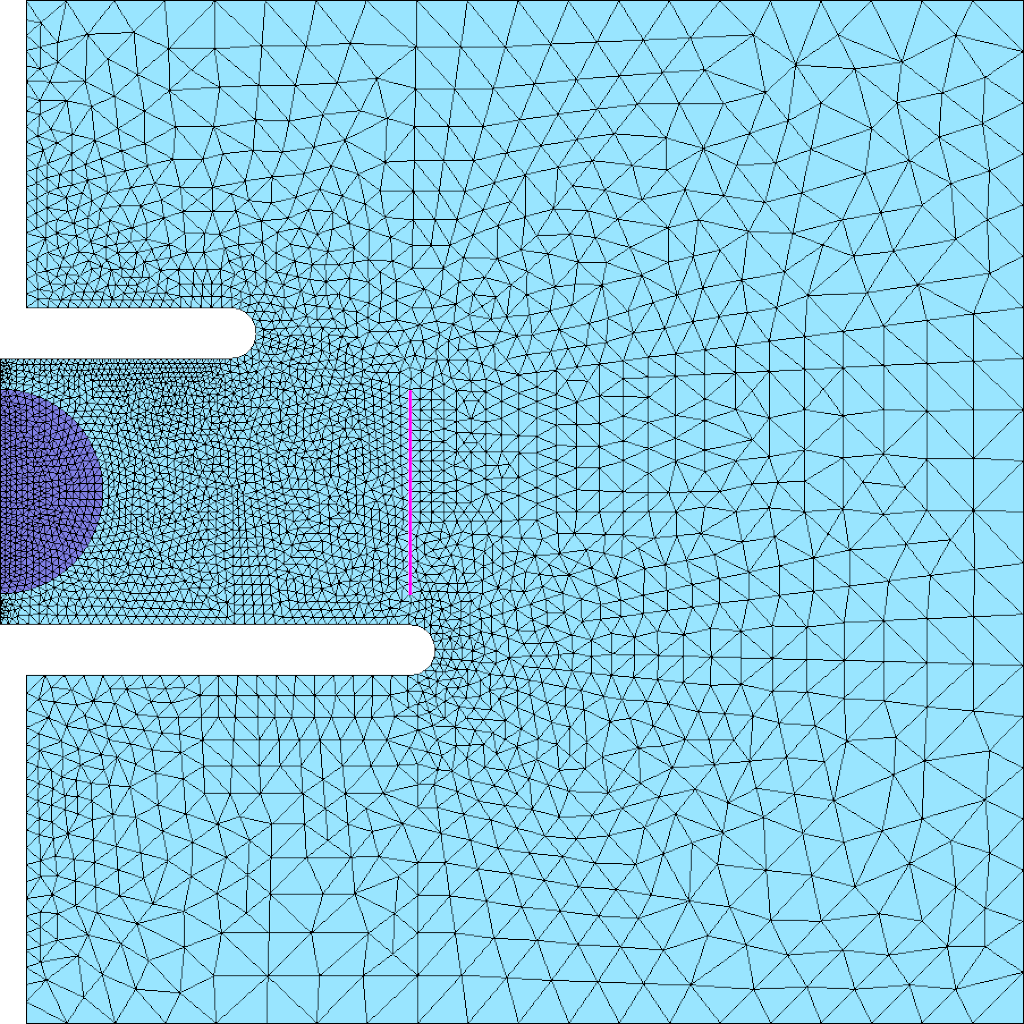
\includegraphics[width=0.45\textwidth]{figs/14}\hfill
\end{Verbatim}

\begin{itemize}
\item The geometry is defined as a collection of counterclockwise oriented segments in parametric form, that is, $\{(x,y)\in\mathbb{R}^2:x=f(t),~y=g(t),~t\in[a,b]\}$, with each segment being a \verb!border! object. 
\item A \verb!border! object is not allowed to geometrically intersect with another \verb!border! object at an arbitrary point, but only at the starting and ending points. Hence, $\varGamma_\mathrm{S}$ constitutes of three \verb!border! objects.
\item The \verb!borders! are grouped based on distinct boundary conditions with the \verb!label! property; if no boundary condition needs to be imposed, \verb!label! can be omitted.
\item Here, the integer \verb!n! specifies the number of points that are used for discretizing the associated \verb!border! object. The mesh generator uses this discretization for deciding the resolution of the triangulation throughout $\varOmega$.
\item If you suspect that the solution varies rapidly in the vicinity of a particular location, you can introduce an artificial border and discretize that border with sufficiently many points.
\end{itemize}
%%%%%%%%%%%%%%%%%%%%%%%%%%%%%%%%%%%%%%%%%%%%%%%%%%%%%%%%%%%%%%%%%%%%%%%%%%%%%%%%

\vspace*{0.2cm}
\textbf{3.2 Extracting and modifying domain indicators}
\begin{Verbatim}[commandchars=\\\{\}]
int airDef = T(0.5 , 0.5).region; // default indicator for air
int objDef = T(0.05, 0.5).region; // default indicator for object
cout << "USER/ Default indicator for air   : " << airDef << endl;
cout << "USER/ Default indicator for object: " << objDef << endl;
int[int] newIndicators = [airDef, 3, objDef, 4]; // new indicators
T = change(T, region = newIndicators);
int airNew = T(0.5 , 0.5).region;
int objNew = T(0.05, 0.5).region;
cout << "USER/ New indicator for air must be 3   : " << airNew << endl;
cout << "USER/ New indicator for object must be 4: " << objNew << endl;
\dotfill
USER/ Default indicator for air   : 0
USER/ Default indicator for object: 7
USER/ New indicator for air must be 3   : 3
USER/ New indicator for object must be 4: 4
\end{Verbatim}

\begin{itemize}
\item The method \verb!region! extracts the domain indicator that is automatically assigned to an arbitrary point \verb!x0!, \verb!y0! in a subdomain of a \verb!mesh! object, here, \verb!T(x0,y0).region!. 
\item The function \verb!change! can be used for altering the labels that are associated with nodes, edges, and elements. Here, the option \verb!region! admits an \verb!int[int]! array with the old and new domain indicators.
\end{itemize}
%%%%%%%%%%%%%%%%%%%%%%%%%%%%%%%%%%%%%%%%%%%%%%%%%%%%%%%%%%%%%%%%%%%%%%%%%%%%%%%%

\vspace*{0.2cm}
\textbf{3.3 Defining the permittivity funtion}
\begin{Verbatim}[commandchars=\\\{\}]
real epsAir = 1.0; // relative permittivity value for air
real epsObj = 9.0; // relative permittivity value for object
fespace V0(T, P0);
V0 eps = epsAir*( region == airNew ) + epsObj*( region == objNew );
plot(eps, value = true, fill = true, wait = true);
\end{Verbatim}

\begin{itemize}
\item Since the permittivity function is discontinuous, it must be allowed to have jumps in the FEM setting, and hence, it is defined as a \verb!P0! function.
\end{itemize}
%%%%%%%%%%%%%%%%%%%%%%%%%%%%%%%%%%%%%%%%%%%%%%%%%%%%%%%%%%%%%%%%%%%%%%%%%%%%%%%%

\vspace*{0.2cm}
\textbf{3.4 Computing the potential and the electric field}
\begin{Verbatim}[commandchars=\\\{\}]
// DEFINE, ASSEMBLE, AND SOLVE
varf a(u, v) = int2d(T)( eps*(dx(u)*dx(v) + dy(u)*dy(v)) )
               + on(1, u = 1.0) + on(2, u = 0.0);
varf l(u, v) = on(1, u = 1.0) + on(2, u = 0.0);
fespace V2(T, P2);
matrix A = a(V2, V2);
real[int] b = l(0, V2);
V2 u;
u[] = A^-1*b;
plot(u, fill = true, nbiso = 64, wait = true);

// COMPUTE ELECTRIC FIELD
fespace V1(T, P1);
V1 Ex = -dx(u);
V1 Ey = -dy(u);
V1 Enorm = sqrt(Ex^2 + Ey^2);
plot(Enorm, [Ex, Ey], fill = true, nbiso = 64, wait = true);
\dotfill

\hfill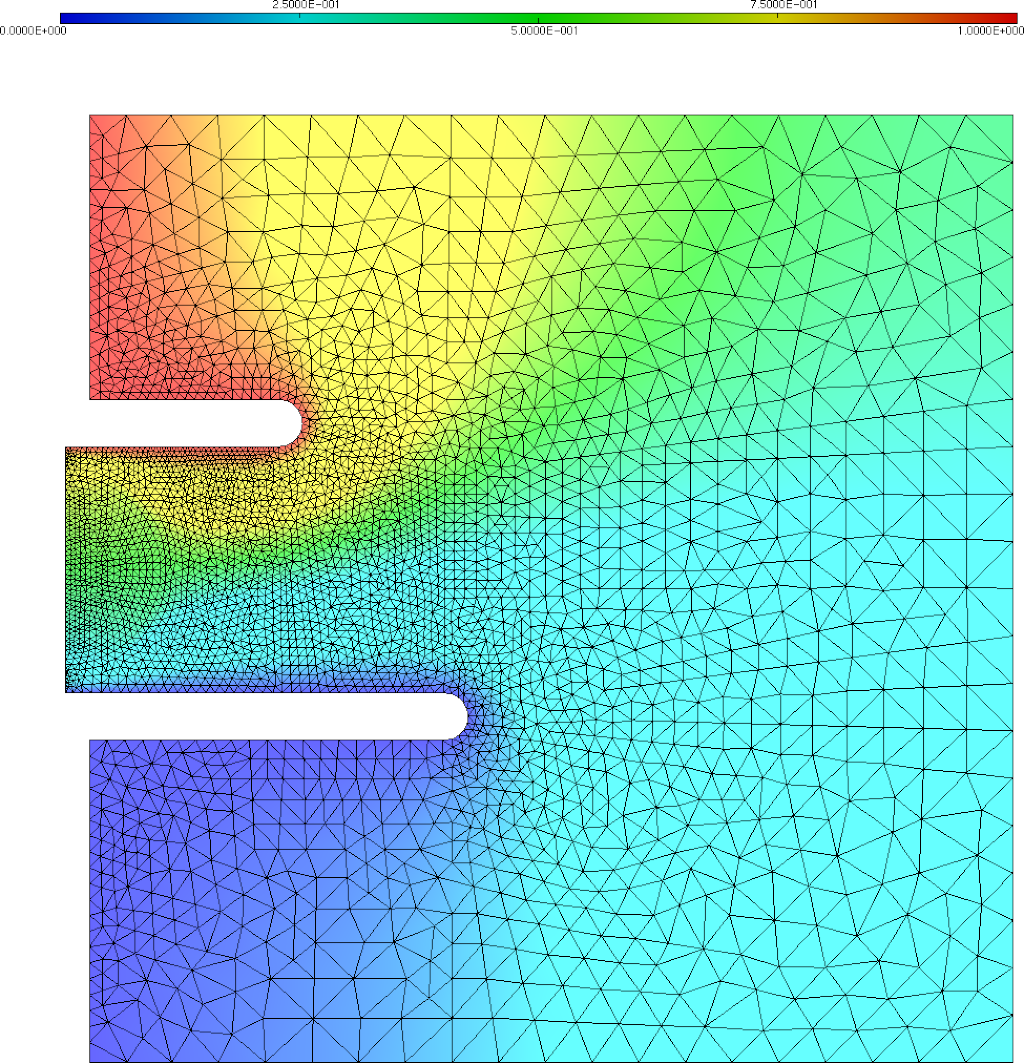
\includegraphics[width=0.45\textwidth]{figs/15}\hfill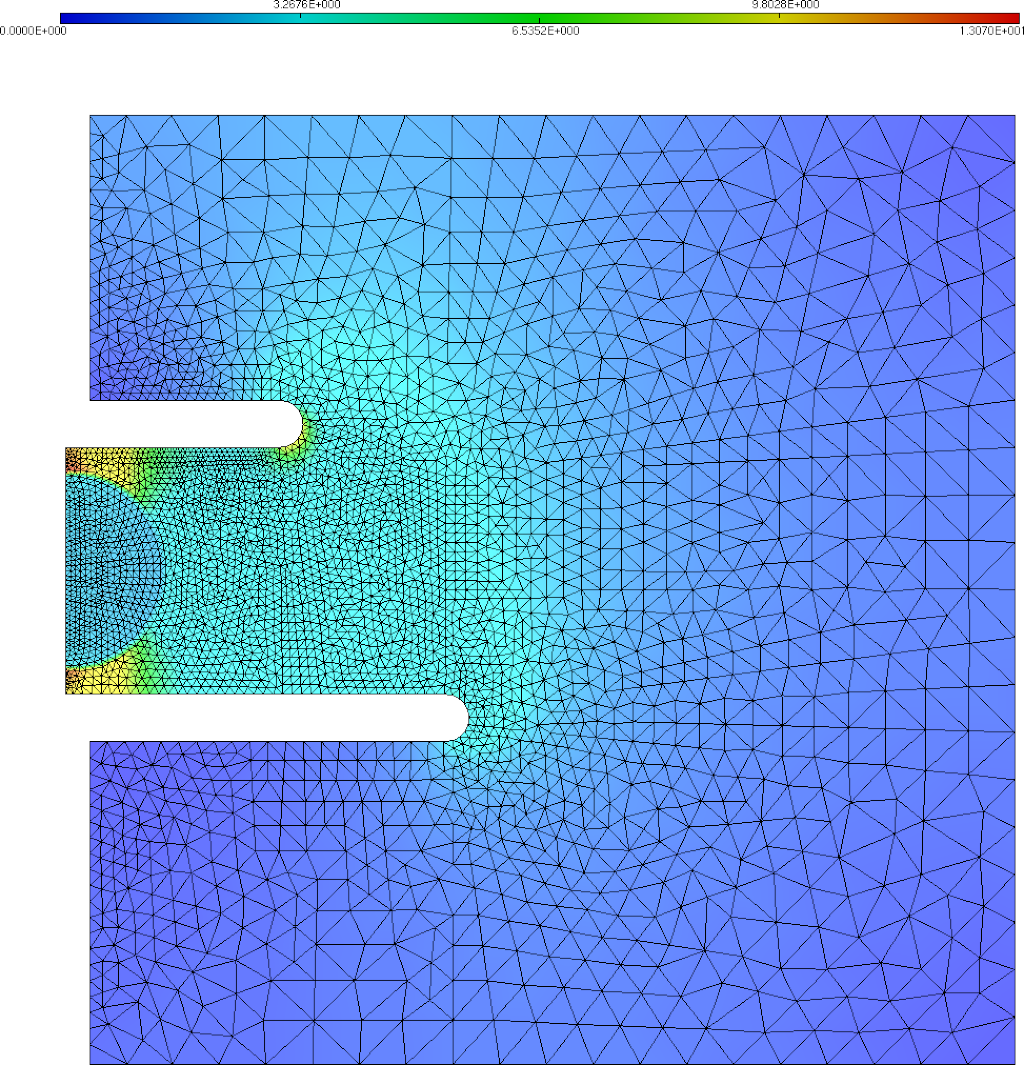
\includegraphics[width=0.45\textwidth]{figs/16}\hfill
\end{Verbatim}

\begin{itemize}
\item As a first debugging approach, it is wise to check that the resulting solution satisfies the boundary conditions. Here, the potential on the boundaries that form the upper terminal is indeed unity, while it is vanishing on the boundaries that form the lower terminal. Further, along the insulating boundary, the gradient of the potential appears to only have non-vanishing tangential component, as expected due to the homogeneous Neumann condition $\partial u/\partial n = 0$.
\item Since the trial space \verb!V2! is build with \verb!P2! elements, the resulting potential is a second-degree polynomial within each element. When computing the electric field, the differentiation reduces the polynomial order to unity, and hence, each component of the electric field is defined to be a \verb!P1! finite element function.
\item The complete example is located at \verb!./code/xmpl-07.edp!.
\end{itemize}
%%%%%%%%%%%%%%%%%%%%%%%%%%%%%%%%%%%%%%%%%%%%%%%%%%%%%%%%%%%%%%%%%%%%%%%%%%%%%%%%

\vspace*{0.2cm}
\textbf{3.5 A three-dimensional capacitor problem in parallel}\\
Here, a three-dimensional variant of \verb!T! is generated by rotation. Then, surface and domain indicators that are needed for imposing boundary conditions and for defining the permittivity function, respectively, are extracted from the three-dimensional mesh. As previously, minor modifications are needed for solving the formulated problem with PETSc, in a domain decomposition setting. The solutions that are local to distinct processes are collected to a single process and \verb!medit! is used for visualization. 
\begin{Verbatim}[commandchars=\\\{\}]
// ROTATE 2D MESH AROUND Z AXIS
mesh3 T3 = buildlayers(T, 40, zbound    = [0, -2.0*pi],
                              transfo   = [x*cos(z), x*sin(z), y],
                              facemerge = true);
medit("Mesh", T3);
\dotfill

\hfill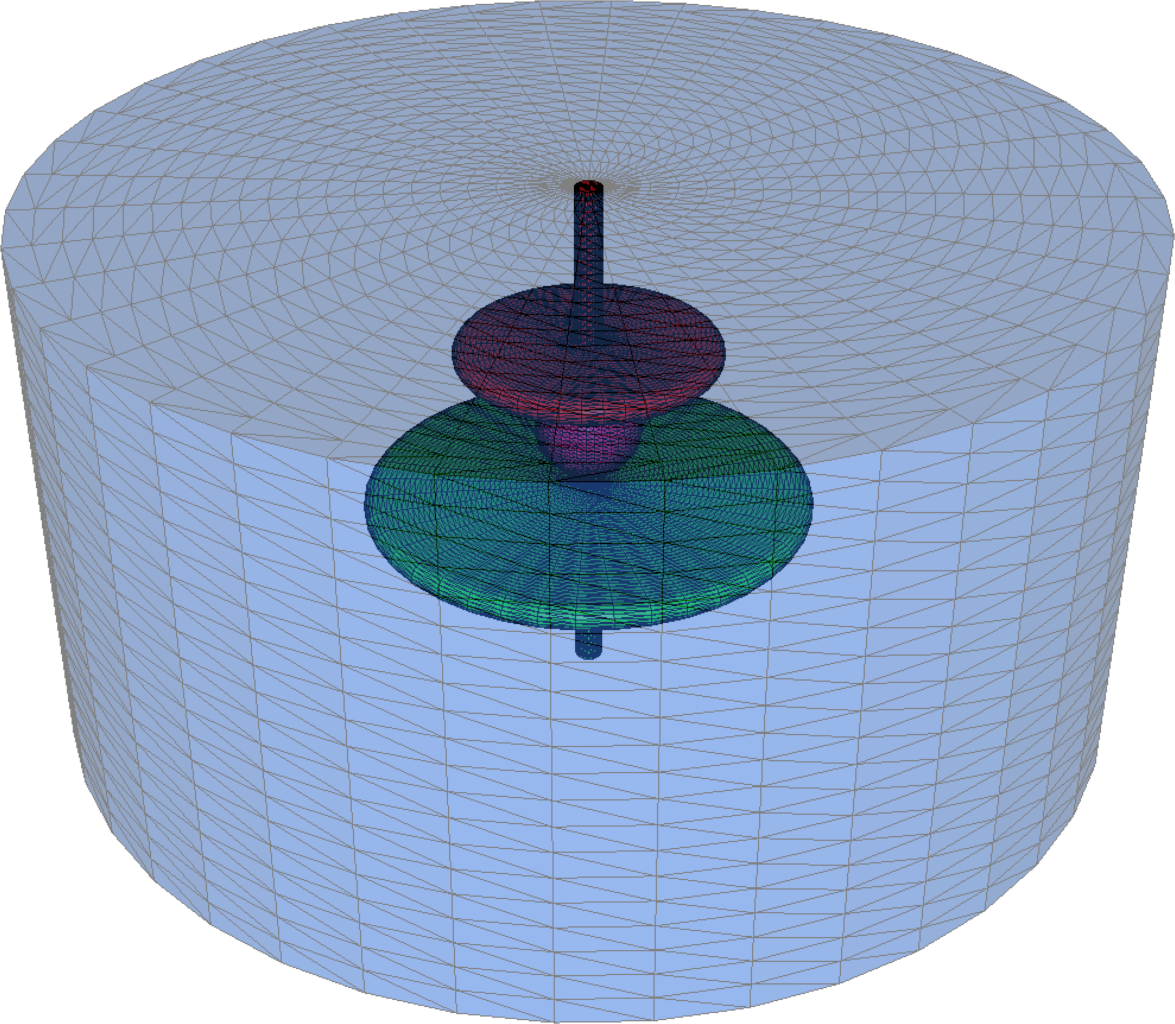
\includegraphics[width=0.45\textwidth]{figs/17}\hfill
\end{Verbatim}

\begin{itemize}
\item The second option of \verb!buildlayers! determines the number of tetrahedra strips to be used for covering the \verb!mesh3! object, \verb!transfo! is used for defining the transformation of the two-dimensional space, while \verb!facemerge! allows the faces of the tetrahedra to be merged, if required. Here, if \verb!facemerge! is set to \verb!false!, then an additional boundary is formed on the symmetry cut.
\item When the \verb!medit! window appears, press \verb!b! to change the background color to white and \verb!F1! to enable a surface cut view. Right-click while the mouse cursor is in the \verb!medit! window and select \verb!Shading+lines! from the \verb!Render mode! option. The \verb!+! and \verb!-! keys can be used for zooming in and out, respectively.
\item To find out what FreeFEM knows about the domain and surface indicators that are associated with the three-dimensional mesh, use the follwoing code snippet.
\end{itemize}

\begin{Verbatim}[commandchars=\\\{\}]
// CHECK BOUNDARY AND DOMAIN INDICATORS OF 3D MESH
int currentBnd;                           // define before varf
int[int] bndLabels = labels(T3);          // array with surface labels
cout << "USER/ Array size: " << bndLabels << endl;
varf onBnd(u, v) = on(currentBnd, u = 1.0);
fespace V1(T3, P1);
V1 bnd;
for ( int cnt = 0; cnt < bndLabels.n; cnt++ ) \{
  currentBnd = bndLabels[cnt];            // update before assembling
  bnd[] = onBnd(0, V1, tgv = -1);
  cout << "USER/ Current boundary label: " << currentBnd << endl;
  medit("Boundary", T3, bnd);
\}

cout << "USER/ Array size: " << regions(T3) << endl;
int air = T3(0.5, 0.0, 0.5).region;
int obj = T3(0.0, 0.0, 0.5).region;
cout << "USER/ Air is labeled   : " << air << endl;
cout << "USER/ Object is labeled: " << obj << endl;
V1 reg = region;                          // P0 for computing but P1
                                          // is ok for visualization
medit("Region", T3, reg);
\dotfill
USER/ Array size: 4
          0       1       2      15
USER/ Current boundary label: 0
USER/ Current boundary label: 1
USER/ Current boundary label: 2
USER/ Current boundary label: 15
USER/ Array size: 2
          0       6
USER/ Air is labeled   : 0
USER/ Object is labeled: 6

\hfill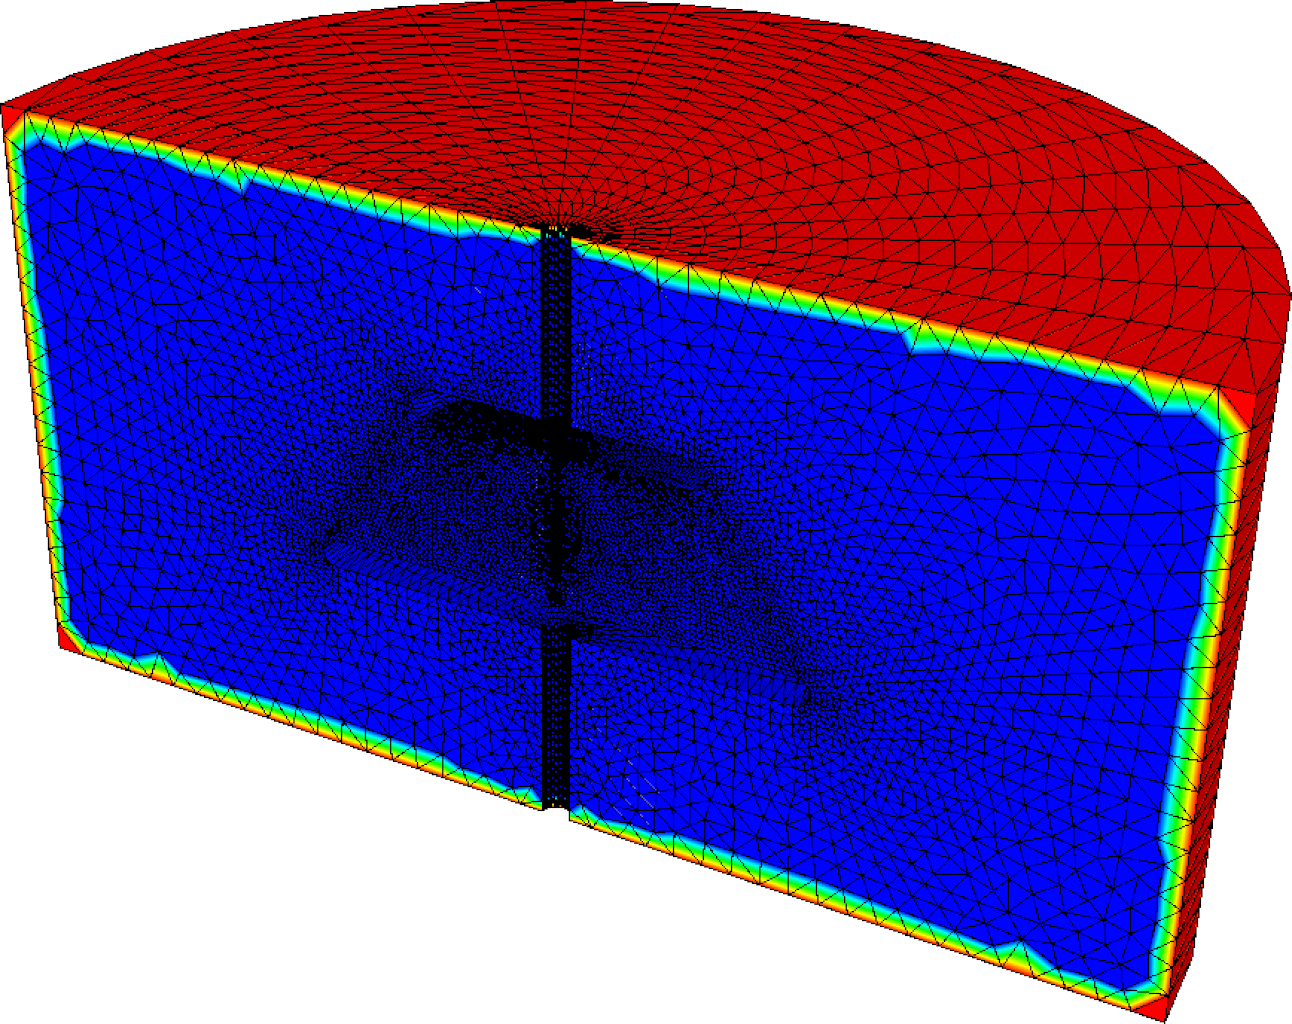
\includegraphics[width=0.45\textwidth]{figs/18}\hfill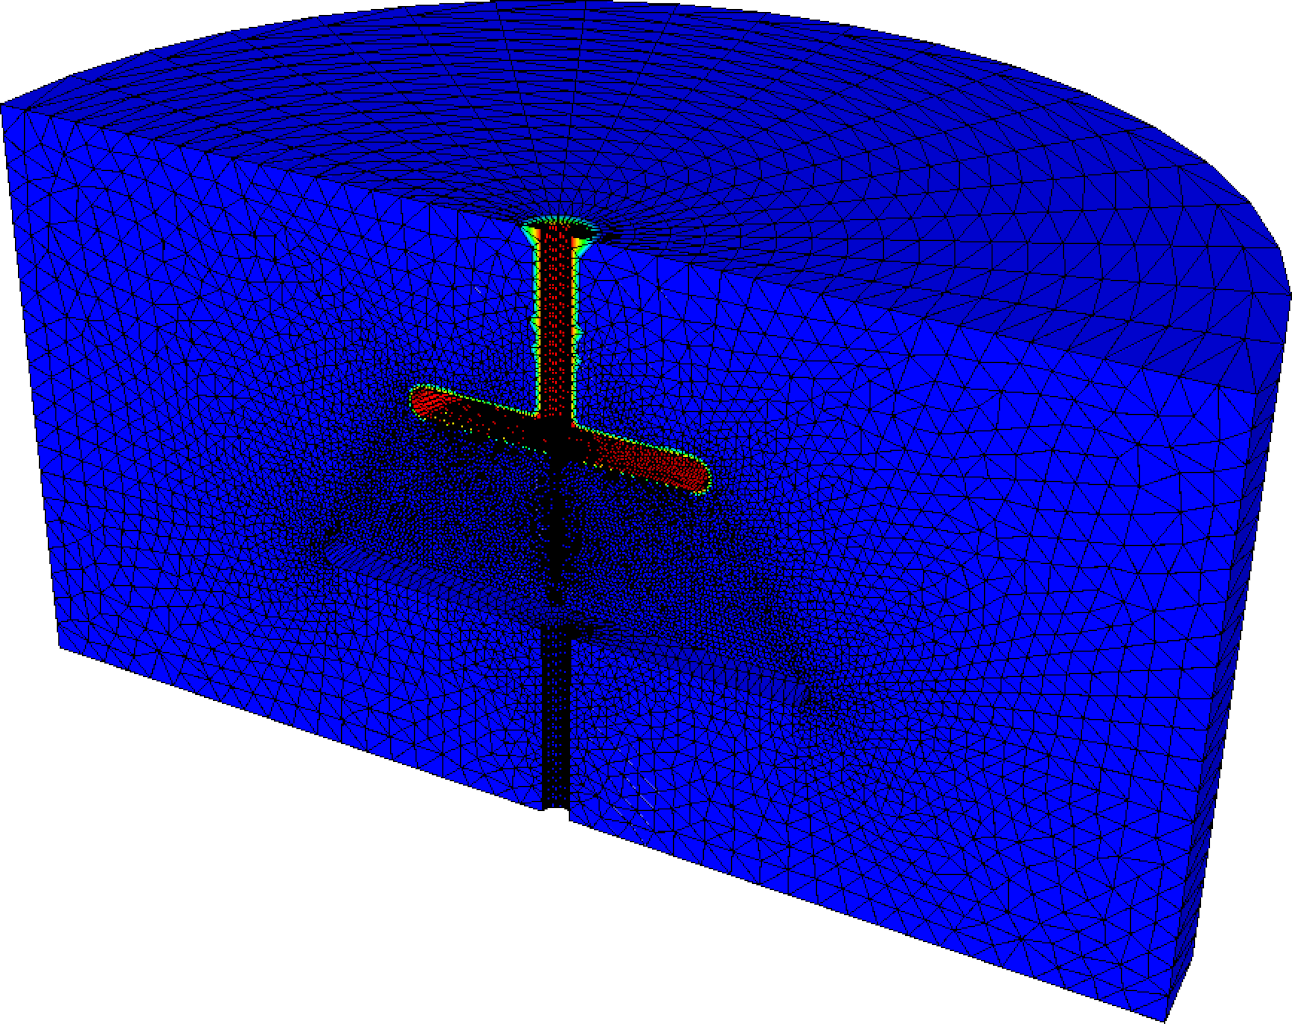
\includegraphics[width=0.45\textwidth]{figs/19}\hfill
\hfill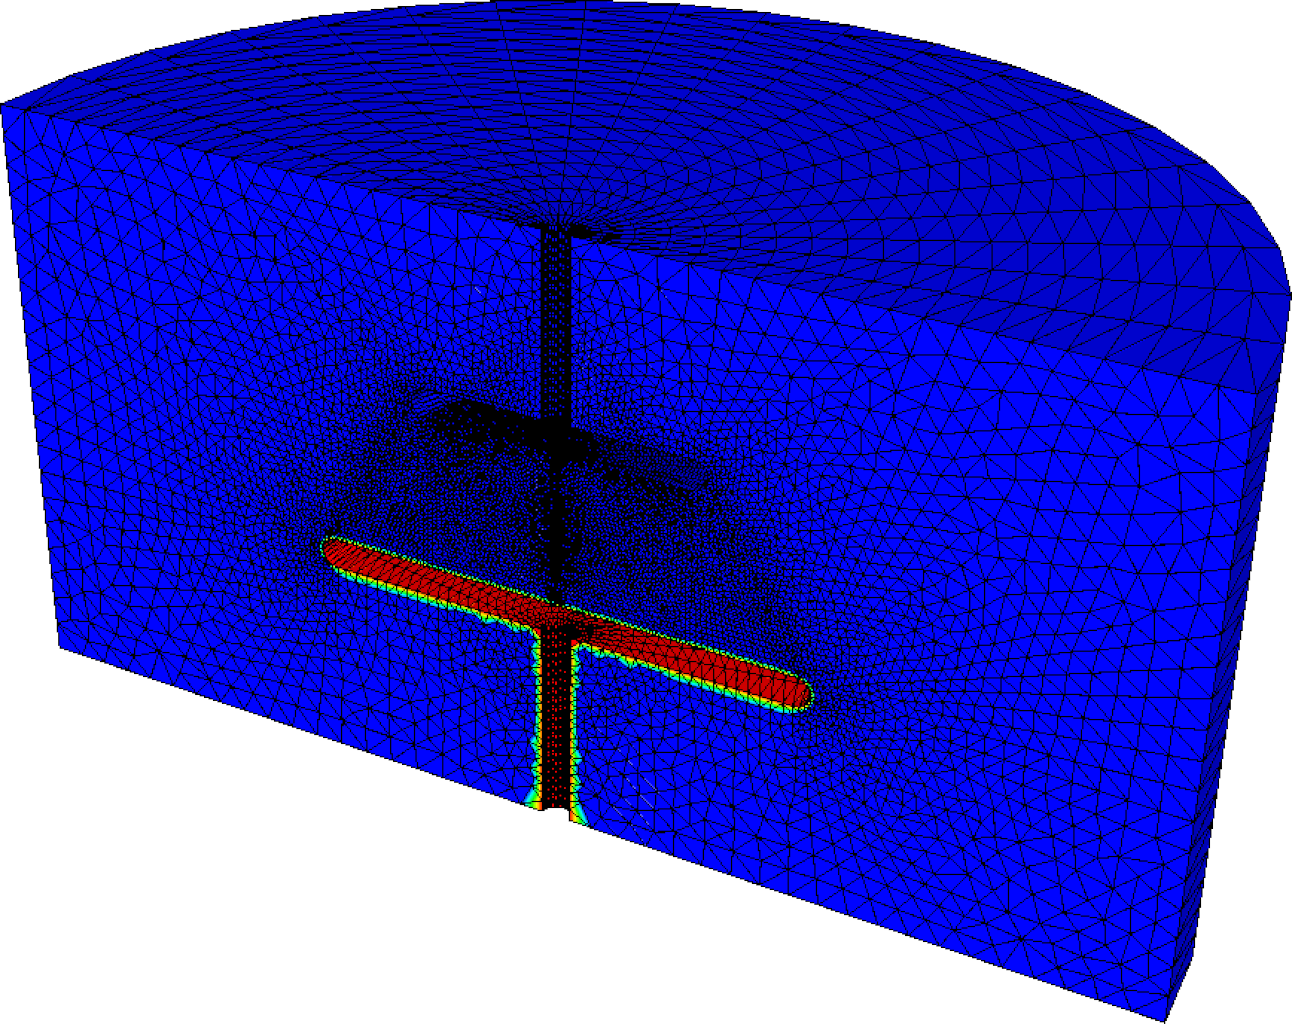
\includegraphics[width=0.45\textwidth]{figs/20}\hfill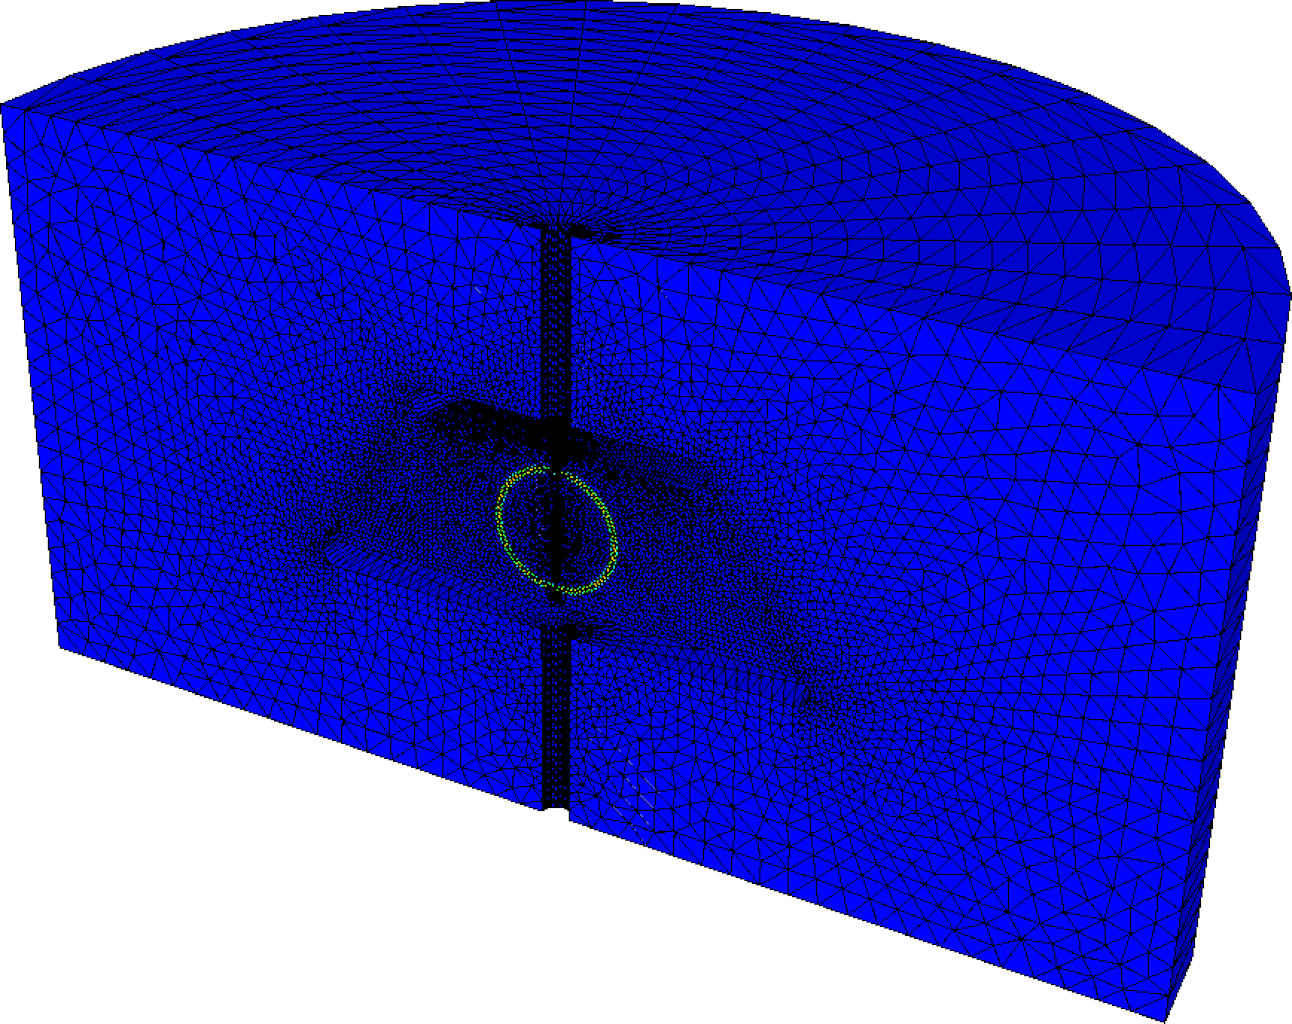
\includegraphics[width=0.45\textwidth]{figs/21}\hfill
\end{Verbatim}

\begin{itemize}
\item The functions \verb!labels! and \verb!regions! return \verb!int[int]! arrays with the surface labels and the domain indicators, respectively.
\item A single \verb!V1! surface function \verb!bnd! can be defined by setting \verb!u = label! in the \verb!varf! definition. Then, the \verb!for! loop can be omitted, and \verb!bnd! is visualized, after being assembled.
\item When the \verb!medit! window appears, hit the \verb!m! key to project the data onto the mesh.
\end{itemize}

\begin{Verbatim}[commandchars=\\\{\}]
Mat A;
createMat(T3, A, P1);
fespace V0(T3, P0);
V0 eps = epsAir*( region == air ) + epsObj*( region == obj );
varf a(u, v) = int3d(T3)( eps*(dx(u)*dx(v) + dy(u)*dy(v) + dz(u)*dz(v)) )
               + on(1, u = 1.0) + on(2, u = 0.0);
varf l(u, v) = on(1, u = 1.0) + on(2, u = 0.0);
fespace V1(T3, P1);
A = a(V1, V1, tgv = -1);
set(A, sparams = "-ksp_type preonly -pc_type lu");
real[int] b = l(0, V1, tgv = -1);
V1 u;
u[] = A^-1*b;
medit("Local solutions", T3, u);
\dotfill

\hfill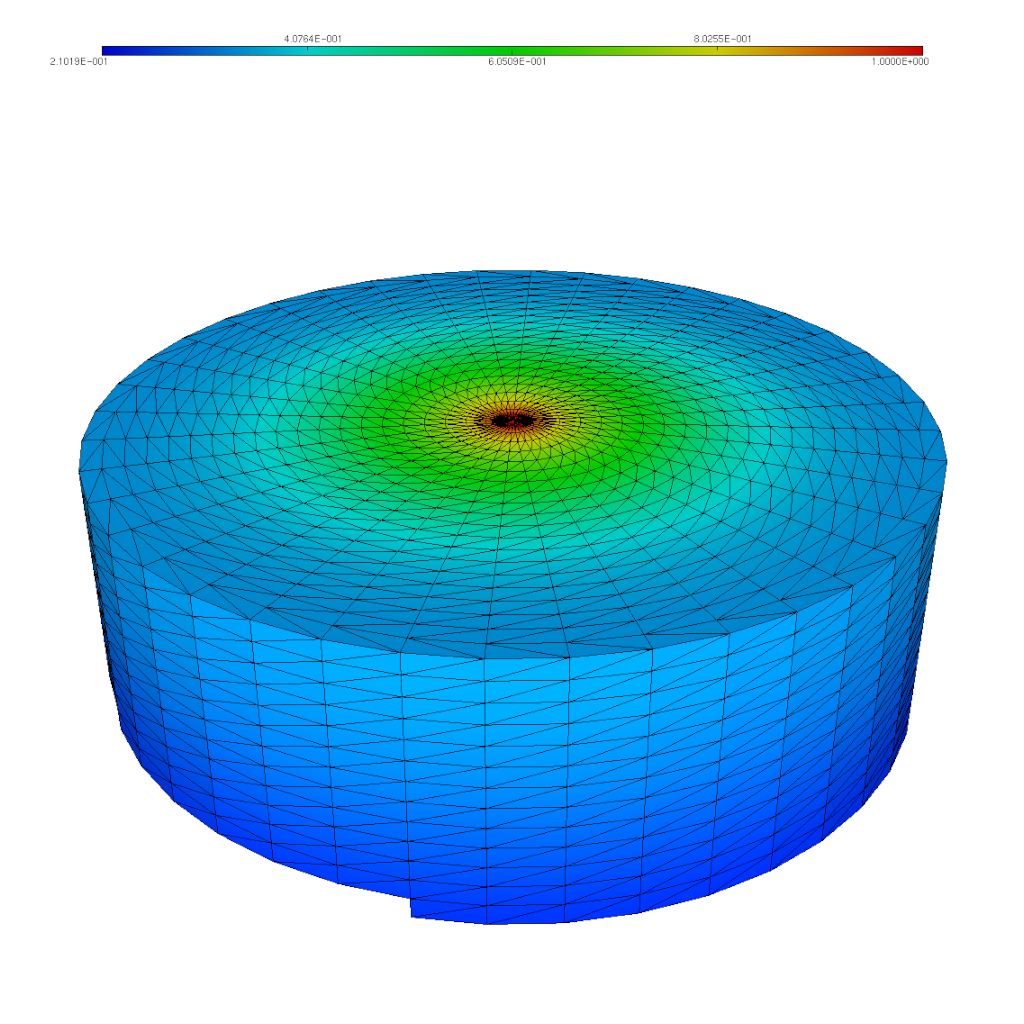
\includegraphics[width=0.45\textwidth]{figs/23}\hfill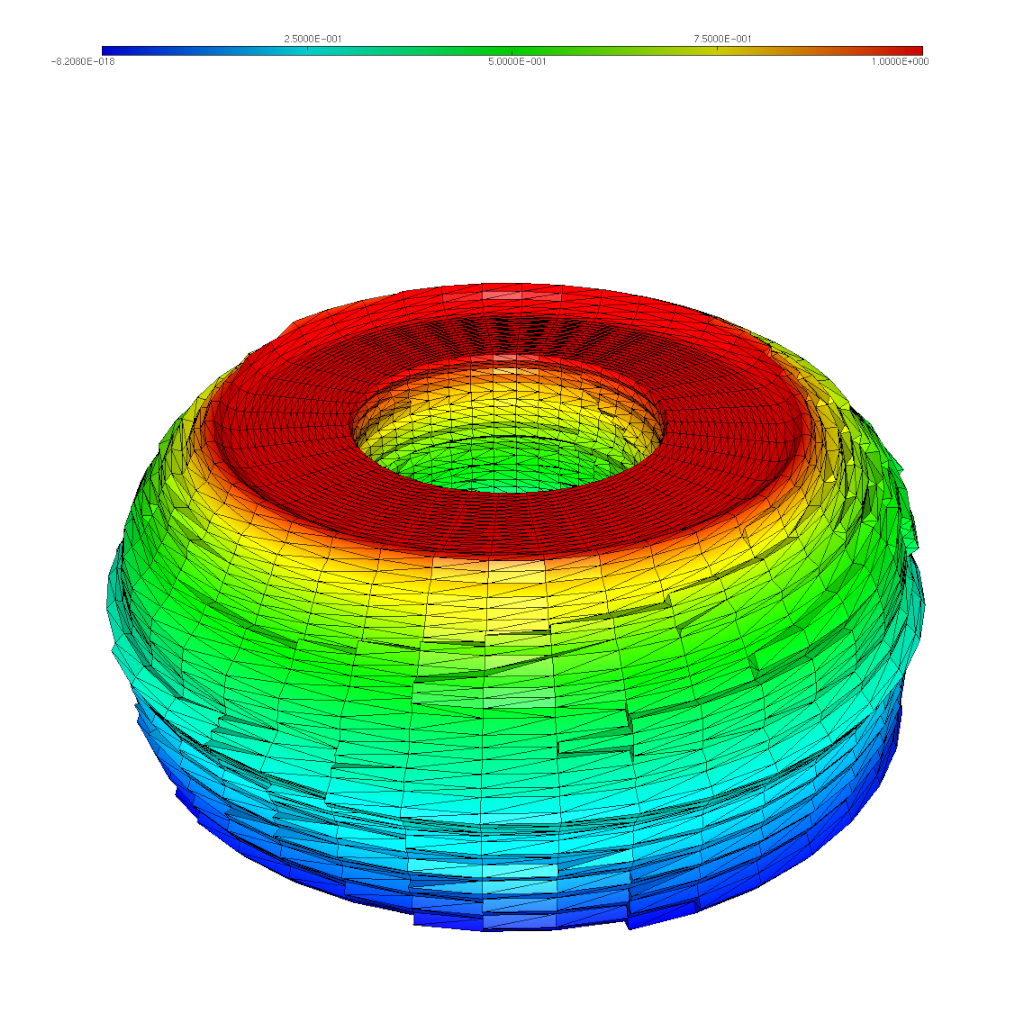
\includegraphics[width=0.45\textwidth]{figs/24}\hfill
\hfill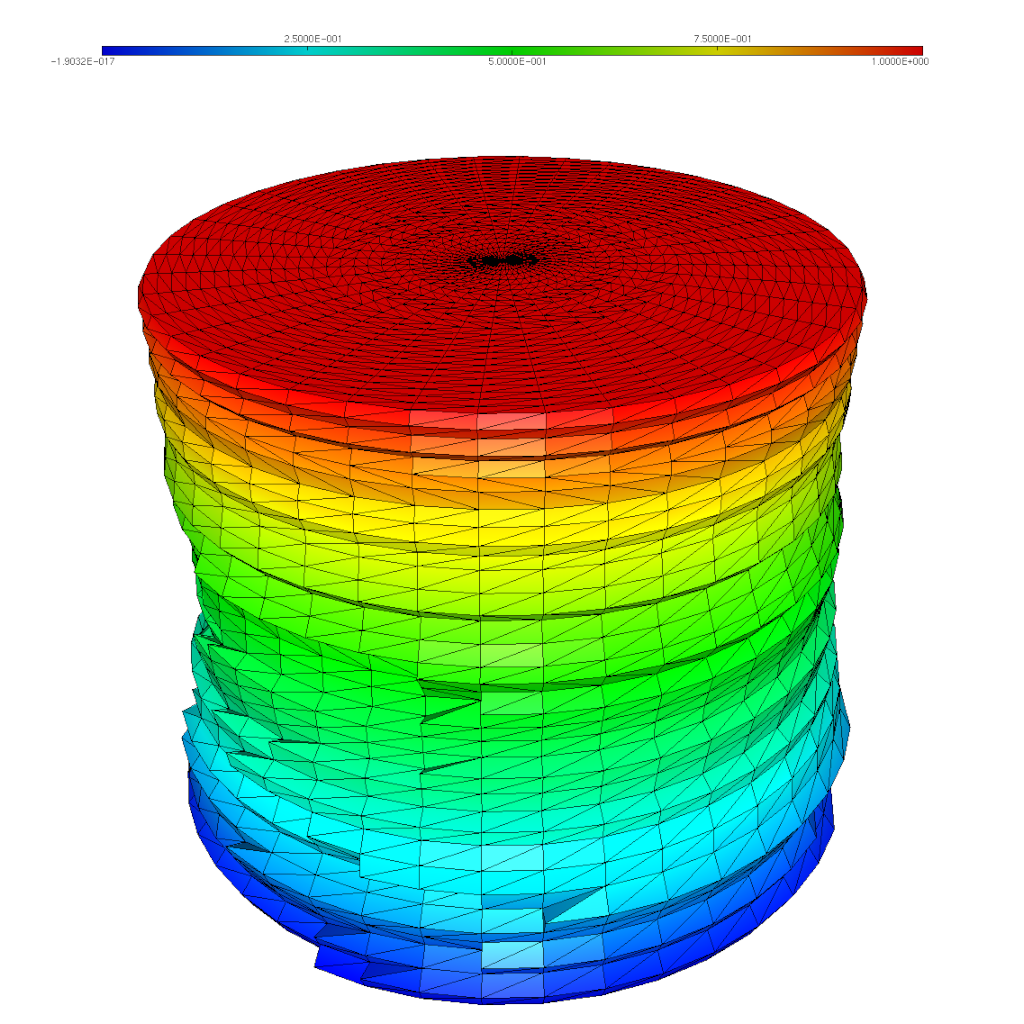
\includegraphics[width=0.45\textwidth]{figs/25}\hfill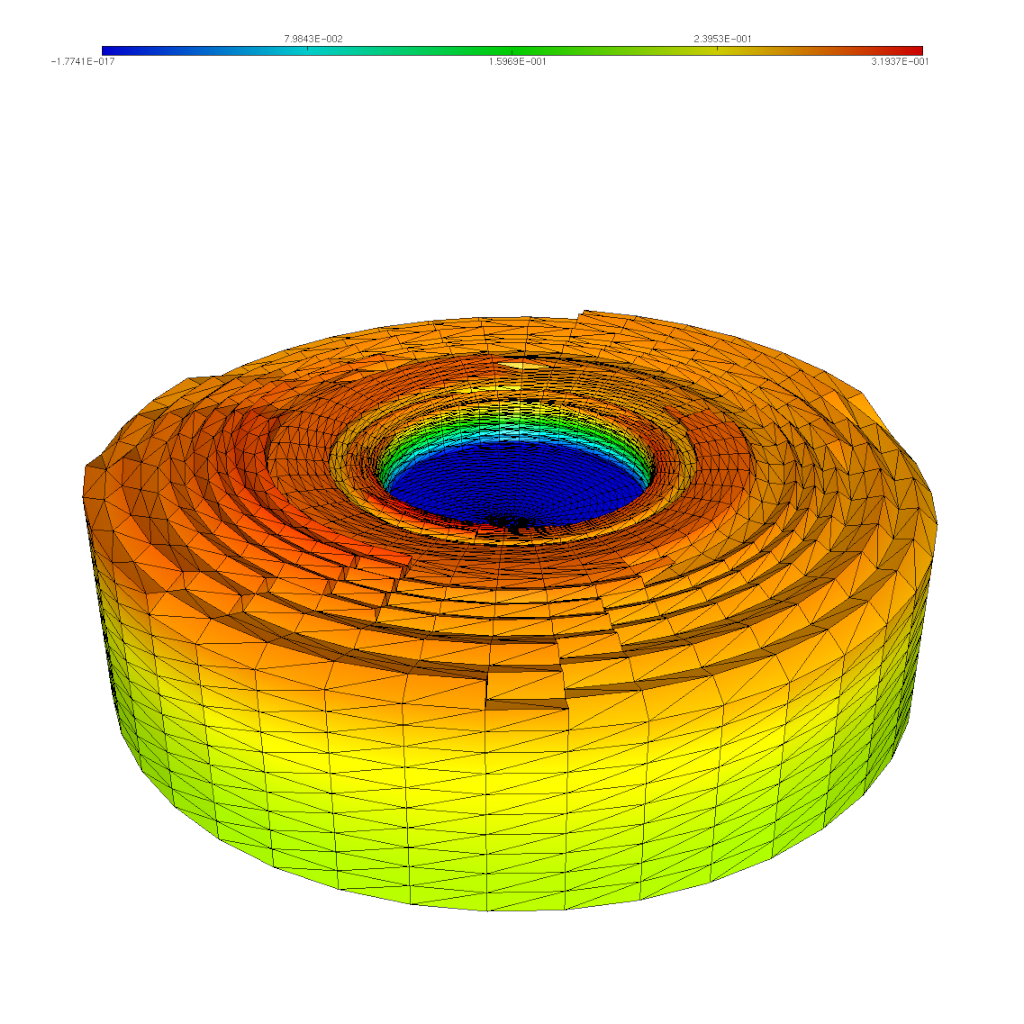
\includegraphics[width=0.45\textwidth]{figs/26}\hfill
\end{Verbatim}

\begin{itemize}
\item This part of the code is similar to the cube example in \S1.6, but in addition, PETSc parameters are passed with the \verb!set! function. The \verb!-ksp_type! option determines the solver, while the \verb!-pc_type! specifies the preconditioning method. Here, \verb!preonly! instructs PETSc not to use a Krylov space solver, since the solution is determined by the \verb!lu! preconditioner. This pair of choices corresponds to a direct solver.
\item Since \verb!u! is local to each process, when calling \verb!medit! the result is as shown in the figure above, while more often, the global solution is of interest. To visualize the global solution several modifications are required, before and after distributing the mesh.
\end{itemize}

\begin{Verbatim}[commandchars=\\\{\}]
// BEFORE CALL TO createMat
mesh3 originalMesh = T3; // keep mesh before dd for its numbering
int[int] n2o;            // define a global variable to store the 
                         // mapping between different numberings
macro T3N2O() n2o        // mesh name followed by N20 and the global 
                         // variable you just defined
\end{Verbatim}

\begin{itemize}
\item Since the mesh is modified and distributed by calling \verb!createMat!, or by explicitly calling \verb!buildDmesh(T3)!, the original mesh needs to be stored. To distribute the mesh, the domain decomposition routines perform mesh modifications with the \verb!trunc! function, which admits the option \verb!new2old! for storing  information about how the after-\verb!trunc! numbering maps to the before-\verb!trunc! numbering.
\end{itemize}

\begin{Verbatim}[commandchars=\\\{\}]
// AFTER u = A^-1*b
if ( !NoGraphicWindow ) \{
  real[int] sol;
  changeNumbering(A, u[], sol);                 // FF2PETSc
  changeNumbering(A, u[], sol, inverse = true); // PETSc2FF
  fespace fesPlot(originalMesh, P1);
  int[int] rest = restrict(V1, fesPlot, n2o);
  fesPlot uTmp, uPlot;  
  for[i, j : rest] uTmp[][j] = u[][i];
  mpiReduce(uTmp[], uPlot[], processor(0, mpiCommWorld), mpiSUM);
  if( mpirank == 0 ) \{
    medit("Global solution", originalMesh, uPlot);
  \}
\}
\dotfill

\hfill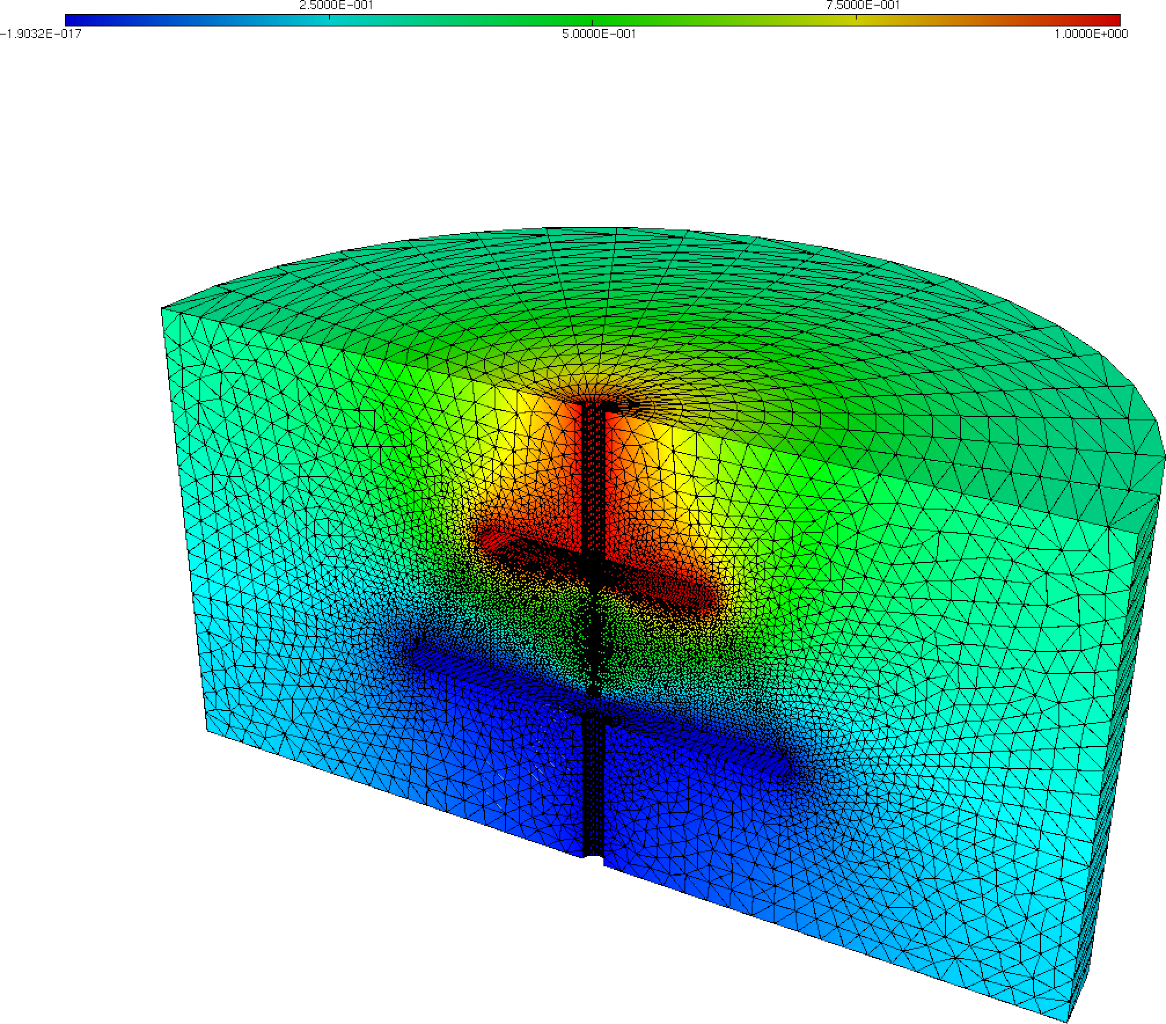
\includegraphics[width=0.45\textwidth]{figs/27}\hfill
\end{Verbatim}

\begin{itemize}
\item In essence, the conditional statement tests a double negation, and hence, to enter this piece of code, the option \verb!-wg! is needed when calling \verb!FreeFem++-mpi!.
\item Since the domain decomposition is overlapping, the FreeFEM numbering has duplicates, whereas for solving with PETSc, each degree of freedom is assigned to a unique process. The first occurrence of \verb!changeNumbering! (subject to change, \verb!ChangeNumbering! in future releases) performs the transition from the FreeFEM numbering to the PETSc numbering. The second call to \verb!changeNumbering! performs the inverse transition, while setting vanishing values to the duplicated degrees of freedom.
\item Then, the \verb!restrict! function is used for determining the degrees of freedom of the global finite element spaces \verb!fesPlot! that are associated with each \verb!V1!, provided the mapping \verb!n2o! that has been generated after calling \verb!createMat!.
\item Finally, the values \verb!u[][i]! of the local solutions are copied to the right locations of the global \verb!fesPlot! functions \verb!uTmp! with an implicit loop, while an additive MPI reduction collects the local \verb!uTmp! functions to the zeroth process, using the variable \verb!uPlot!.
\item The complete example is located at \verb!./code/xmpl-08.edp!.
\end{itemize}
%%%%%%%%%%%%%%%%%%%%%%%%%%%%%%%%%%%%%%%%%%%%%%%%%%%%%%%%%%%%%%%%%%%%%%%%%%%%%%%%

\section{\hrulefill\\Tutorial 4. FE Spaces on Subdomains and Mesh Truncation}
%
\vspace*{0.2cm}
\textbf{4.1 Finite element spaces on subdomains and function extensions}
\begin{Verbatim}[commandchars=\\\{\}]
int n = 50;
border a001(t = 0.0, 2.0*pi)\{ x = 1.0*cos(t); y = 1.0*sin(t); \}
border a002(t = 0.0, 2.0*pi)\{ x = 0.5*cos(t); y = 0.5*sin(t); \}
mesh T = buildmesh( a001(2*n) + a002(n) );

// INNER DOMAIN INDICATOR
int innerDomain = T(0.0, 0.0).region;

// INNER DISK MESH
int[int] n2o;               // mapping between T and TInner
mesh TInner = trunc(T, region == innerDomain, new2old = n2o);
cout << "USER/ Initial mesh  :" << innerDomain << endl;
cout << "USER/ Truncated mesh:" << regions(TInner)[0] << endl;

fespace VInner(TInner, P1); // fespace only in inner domain
VInner v = x*y;             // defined only in inner domain
plot(T, v, fill = true, nbiso = 64, wait = true);

// EXTEND v BY INTERPOLATION
fespace V(T, P1);           // fespace everywhere
V u = v;                    // interpolation in = operator
plot(T, u, fill = true, nbiso = 64, wait = true);

// EXTEND v BY ZEROS
V w = 0.0;
int[int] rest = restrict(VInner, V, n2o); // VInner and V must have
                                          // same type of elements
for[i, j : rest] w[][j] = v[][i];
plot(T, w, fill = true, nbiso = 64, wait = true);

// ELIMINATE THE STRIP OF ELEMENTS OUTSIDE innerDomain
w = w * (region == innerDomain);
plot(T, w, fill = true, nbiso = 64, wait = true);
\dotfill
USER/ Initial mesh domain indicator  :0
USER/ Truncated mesh domain indicator:0

\hfill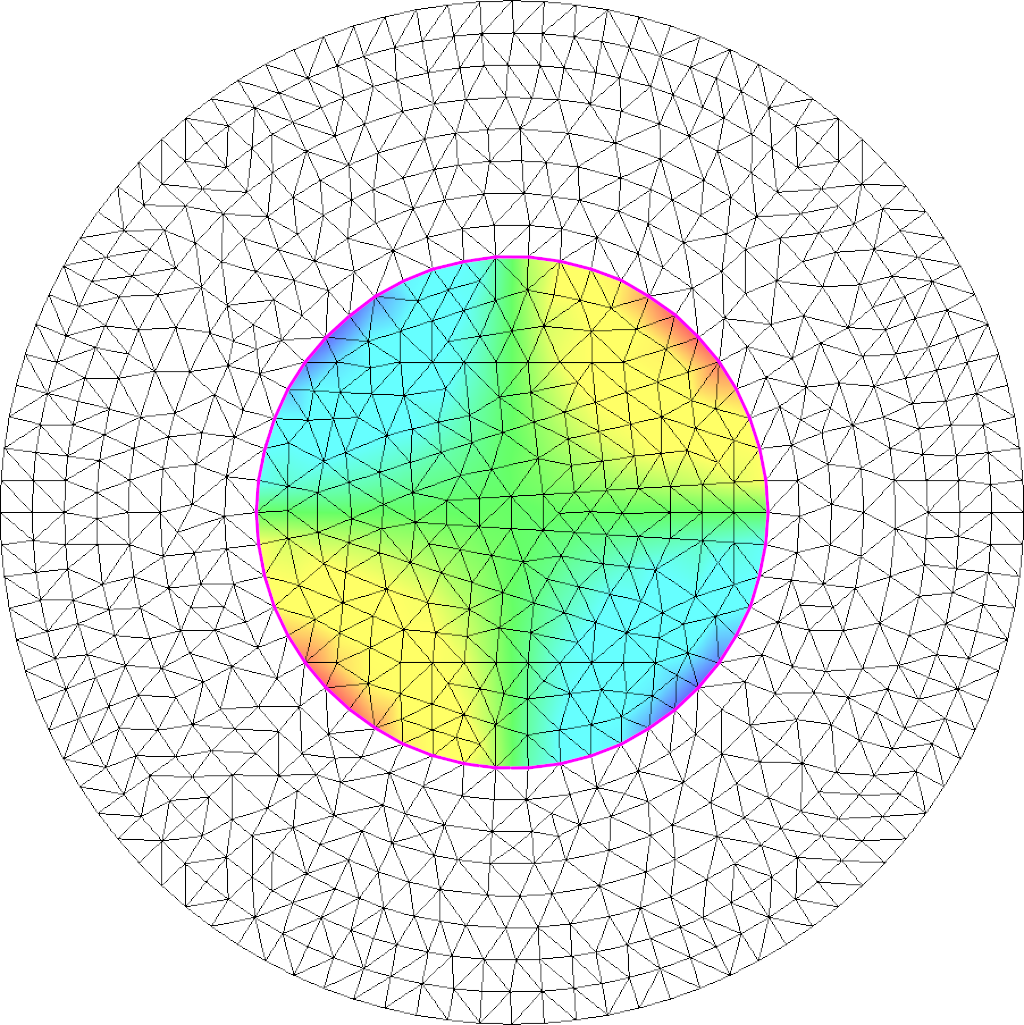
\includegraphics[width=0.45\textwidth]{figs/48}\hfill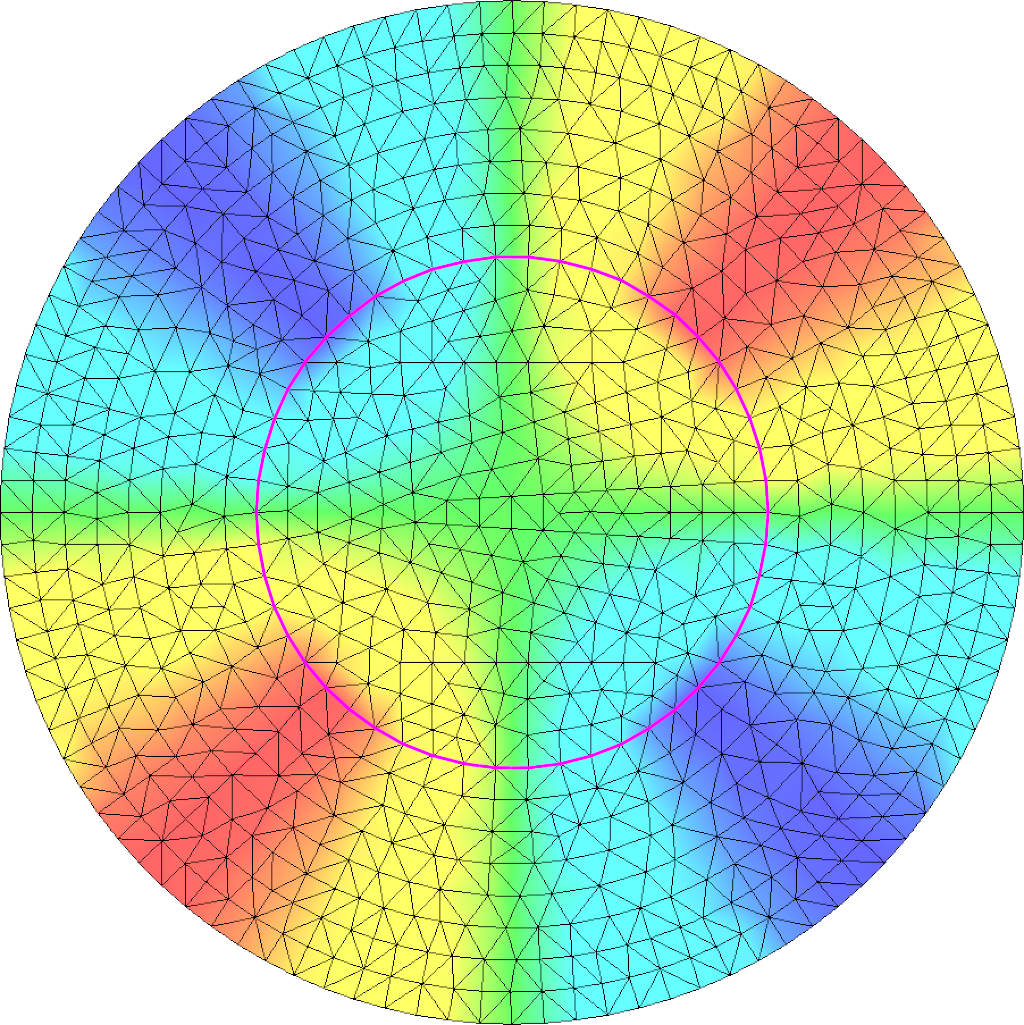
\includegraphics[width=0.45\textwidth]{figs/49}\hfill

\hfill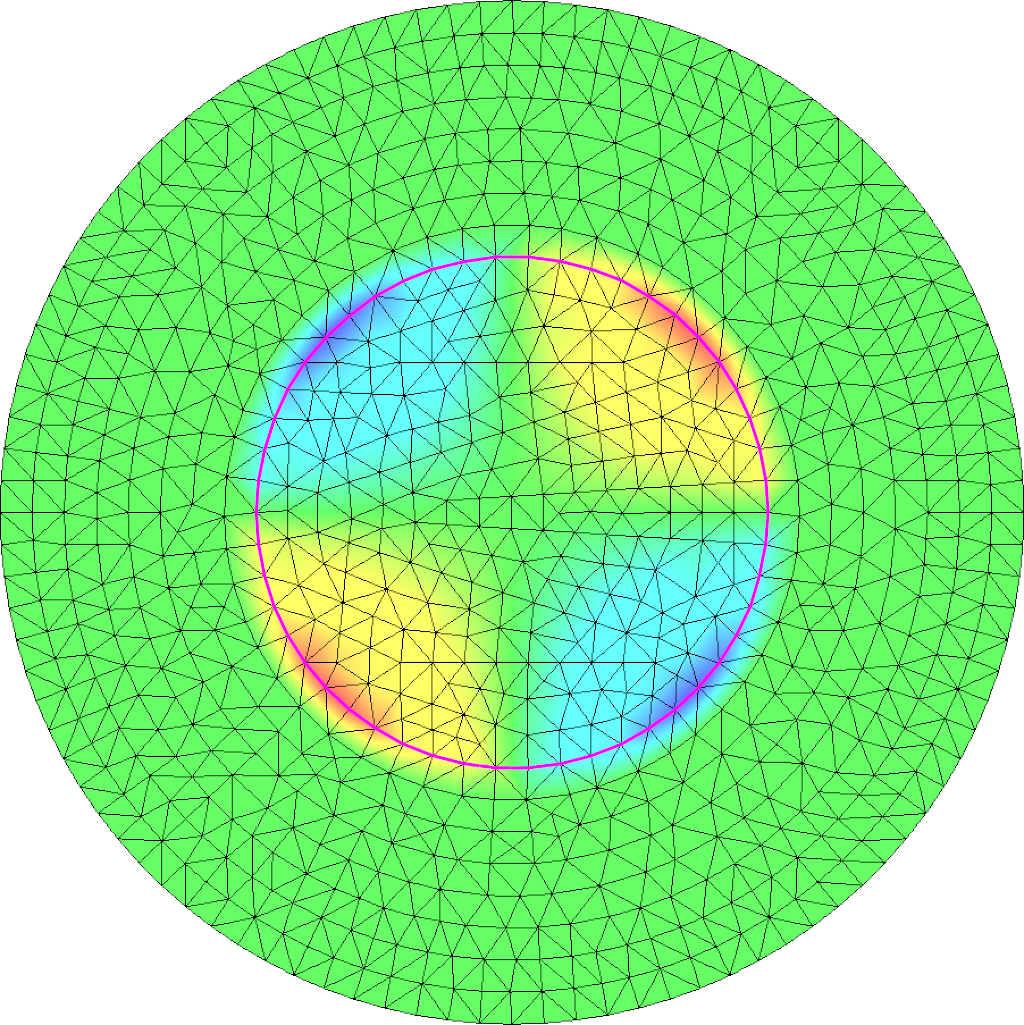
\includegraphics[width=0.45\textwidth]{figs/50}\hfill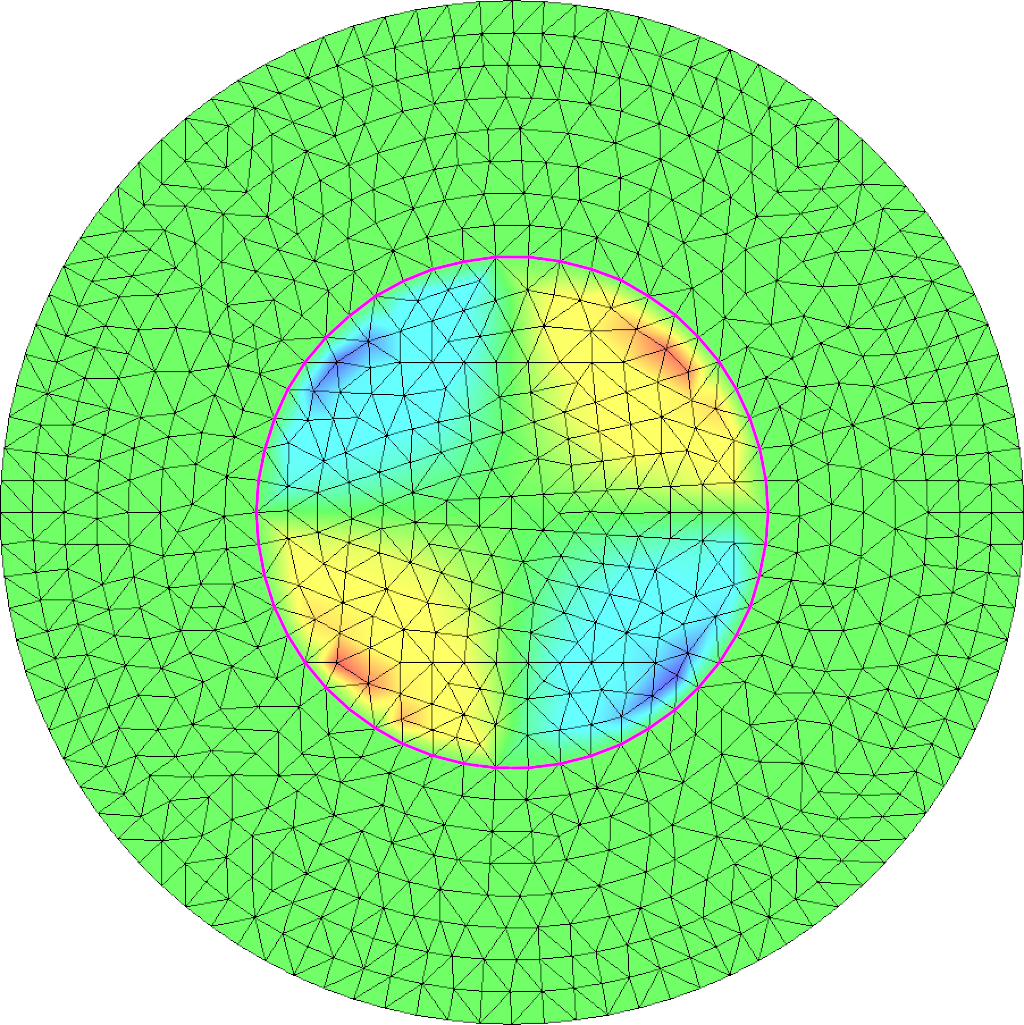
\includegraphics[width=0.45\textwidth]{figs/51}\hfill
\end{Verbatim}
\begin{itemize}
\item The function \verb!v! is defined only in region with domain indicator \verb!innerDomain!. Since \verb!V! is defined over the initial mesh \verb!T!, the operator \verb!=! uses interpolation to extend \verb!v!. If instead of interpolation a vanishing extension is needed, the function \verb!restrict! can be used in combination with an implicit \verb!for! loop.
\item Since \verb!P1! elements are used, it takes a strip of elements for the function \verb!w! to vanish outside the domain with domain indicator \verb!innerDomain!. An artificial boundary, a mesh that is fine in the vicinity of the interior boundary, or a multiplication with the essentially \verb!P0! function \verb!region == innerDomain!, can be used for eliminating or reducing the effect of the leaking values. Be cautious when using the latter approach, since it also modifies the values of \verb!w! inside the domain with \verb!innerDomain!.
\end{itemize}
%%%%%%%%%%%%%%%%%%%%%%%%%%%%%%%%%%%%%%%%%%%%%%%%%%%%%%%%%%%%%%%%%%%%%%%%%%%%%%%%

\vspace*{0.2cm}
\textbf{4.2 A two-dimensional wave propagation problem}\\
Consider the cylindrically symmetric acoustic horn whose cross section is depicted in the figure below, with the circular object within the domain being made of sound-hard material. The  Helmholtz variational boundary value problem of interest reads
\begin{align*}
&\text{<<find }u\in H^1(\varOmega)\text{ such that }&\\
&\int_\varOmega \rho y\nabla u \cdot \nabla v - k^2\int_\varOmega \rho y u v + (\mathrm{i}k+1)\int_{\varGamma_\mathrm{out}} uv + \mathrm{i}k\int_{\varGamma_\mathrm{in}} uv=2\mathrm{i}k\int_{\varGamma_\mathrm{in}}v\\
&\text{for all }v\in H^1(\varOmega)\text{>>}.
\end{align*}
Here, the distance $y$ from the lowest horizontal boundary enters the surface integrals due to the assumed cylindrical symmetry, $k=2\uppi f/c$, with $f=1200~\mathrm{Hz}$ and $c=345~\mathrm{m/s}$, the line integral along the space truncating boundary $\varGamma_\mathrm{out}$ corresponds to the lowest order Enquist–Majda condition, and the line integrals along $\varGamma_\mathrm{in}$ impose a right-traveling wave of unity amplitude in the waveguide, while leaving unaltered the left-traveling waves that are caused by reflections. The scatterer is modeled in two different ways. First, by incorporating the domain $S$ in the computational domain and setting $\rho|\varOmega\setminus\overline{S}=1$ and $\rho|S=10^{-8}$, and second by introducing a hole in the corresponding region of the computational domain and imposing a homogeneous Neumann condition on the resulting boundary, in which case $\rho|\varOmega=1$.
%
\begin{center}
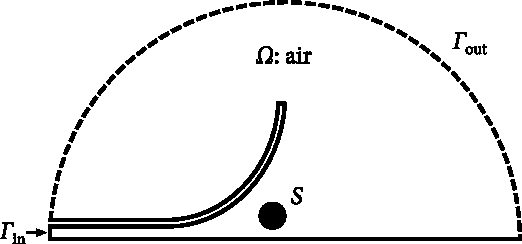
\includegraphics[width=0.45\textwidth]{figs/30}
\end{center}
%
\begin{Verbatim}[commandchars=\\\{\}]
include "xmpl-09-geo.idp"
int n = 10;
mesh T = buildmesh(a001(16*n) + a002(16*n) + a003(4*n) +
                   a004(4*n)  + a005(n/5)  + a006(8*n) +
                   a007(4*n)  + a008(n)    + a009(8*n));

int air = T(1.000, 0.900).region;
int obj = T(0.950, 0.100).region;
fespace V0(T, P0);
V0 rho = 1.0*( region == air ) + 1.0e-8*( region == obj );

real k = 2.0*pi*1200/345.0;
varf a(u, v) = int2d(T)( rho*y*(dx(u)*dx(v) + dy(u)*dy(v)) )
             + int2d(T)(-rho*y*k*k*u*v )
             + int1d(T, absorbBndLabel)( 1.0i*k*u*v + u*v )
             + int1d(T, sourceBndLabel)( 1.0i*k*u*v );
varf l(u, v) = int1d(T, sourceBndLabel)( 2.0i*k*v );

fespace V2(T, P2);
matrix<complex> AOnT = a(V2, V2);
complex[int] bOnT = l(0, V2);
V2<complex> uOnT;
uOnT[] = AOnT^-1*bOnT;

V2 uOnTReal = real(uOnT);
plot(uOnTReal, value = true, fill = true, nbiso = 64, wait = true);
\dotfill

\hfill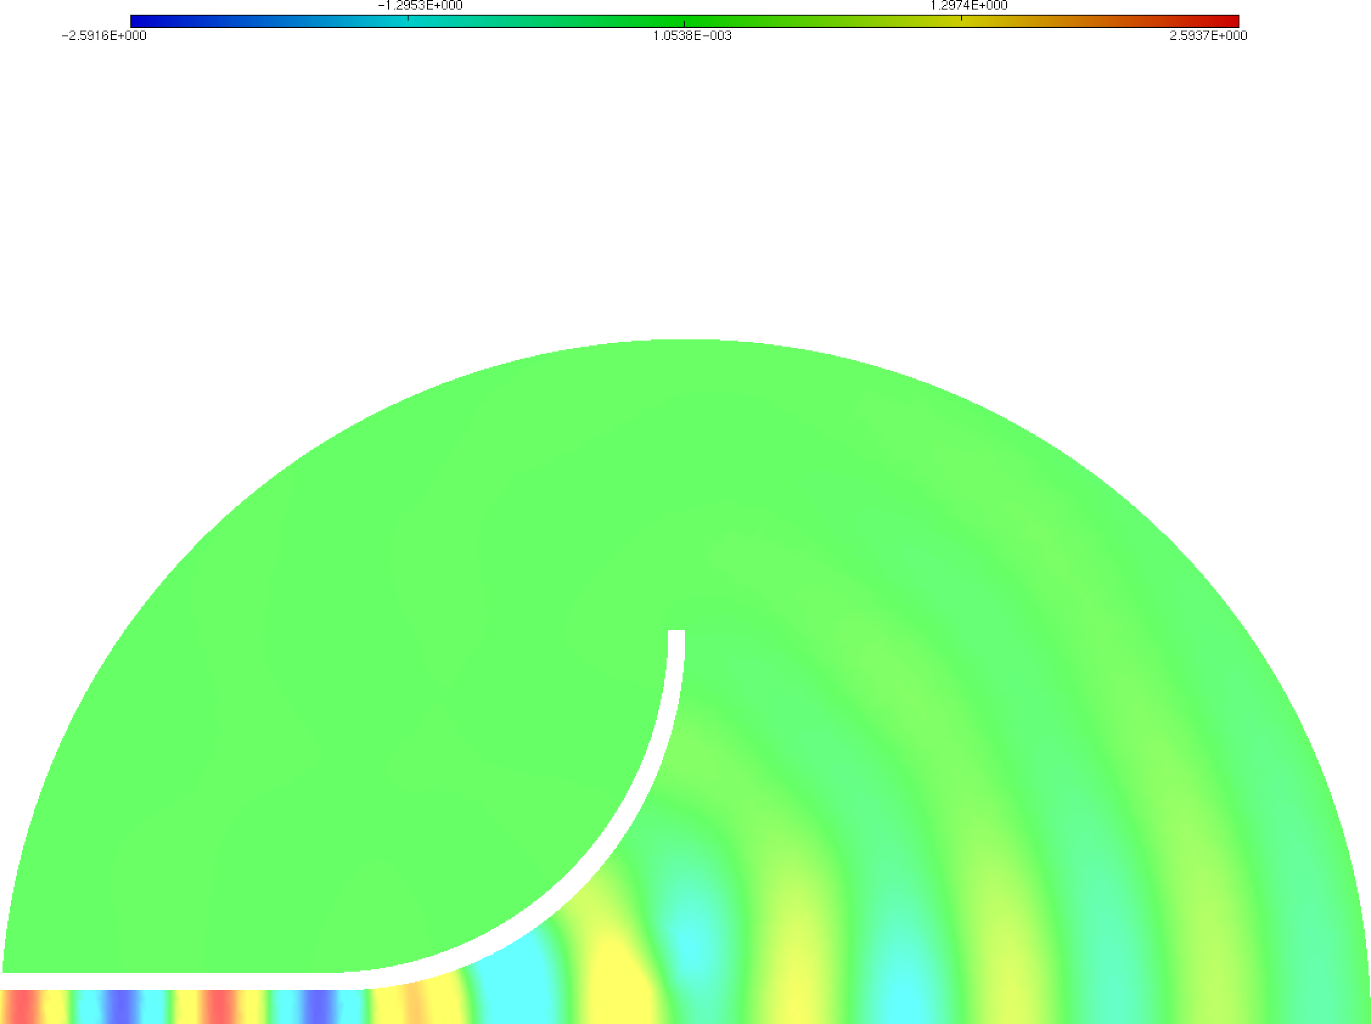
\includegraphics[width=0.45\textwidth]{figs/31}\hfill
\end{Verbatim}

\begin{itemize}
\item The boundary labels and the boundary are separately defined in \verb!xmpl-09-geo.idp!.
\item The finite element function \verb!u!, the matrix associated with the bilinear form, and the right-hand-side vector need to be defined over the complex field, with \verb!V2<complex>!, \verb!matrix<complex>!, and \verb!complex[int]!, respectively.  
\end{itemize}
%%%%%%%%%%%%%%%%%%%%%%%%%%%%%%%%%%%%%%%%%%%%%%%%%%%%%%%%%%%%%%%%%%%%%%%%%%%%%%%%

\textbf{4.3 The two-dimensional problem with $S\not\subset\varOmega$}
\begin{Verbatim}[commandchars=\\\{\}]
int[int] n2o;
T = trunc(T, region == air, label = unusedBndLabel, new2old = n2o);
rho = 1.0; // redefine rho on the new V0 fespace on new mesh
           // not needed but makes the code more transparent
matrix<complex> AOnTt = a(V2, V2);
complex[int] bOnTt = l(0, V2);
V2<complex> uOnTt;
uOnTt[] = AOnTt^-1*bOnTt;
V2 uOnTtReal = real(uOnTt);
plot(uOnTtReal, value = true, fill = true, nbiso = 64, wait = true);
\dotfill

\hfill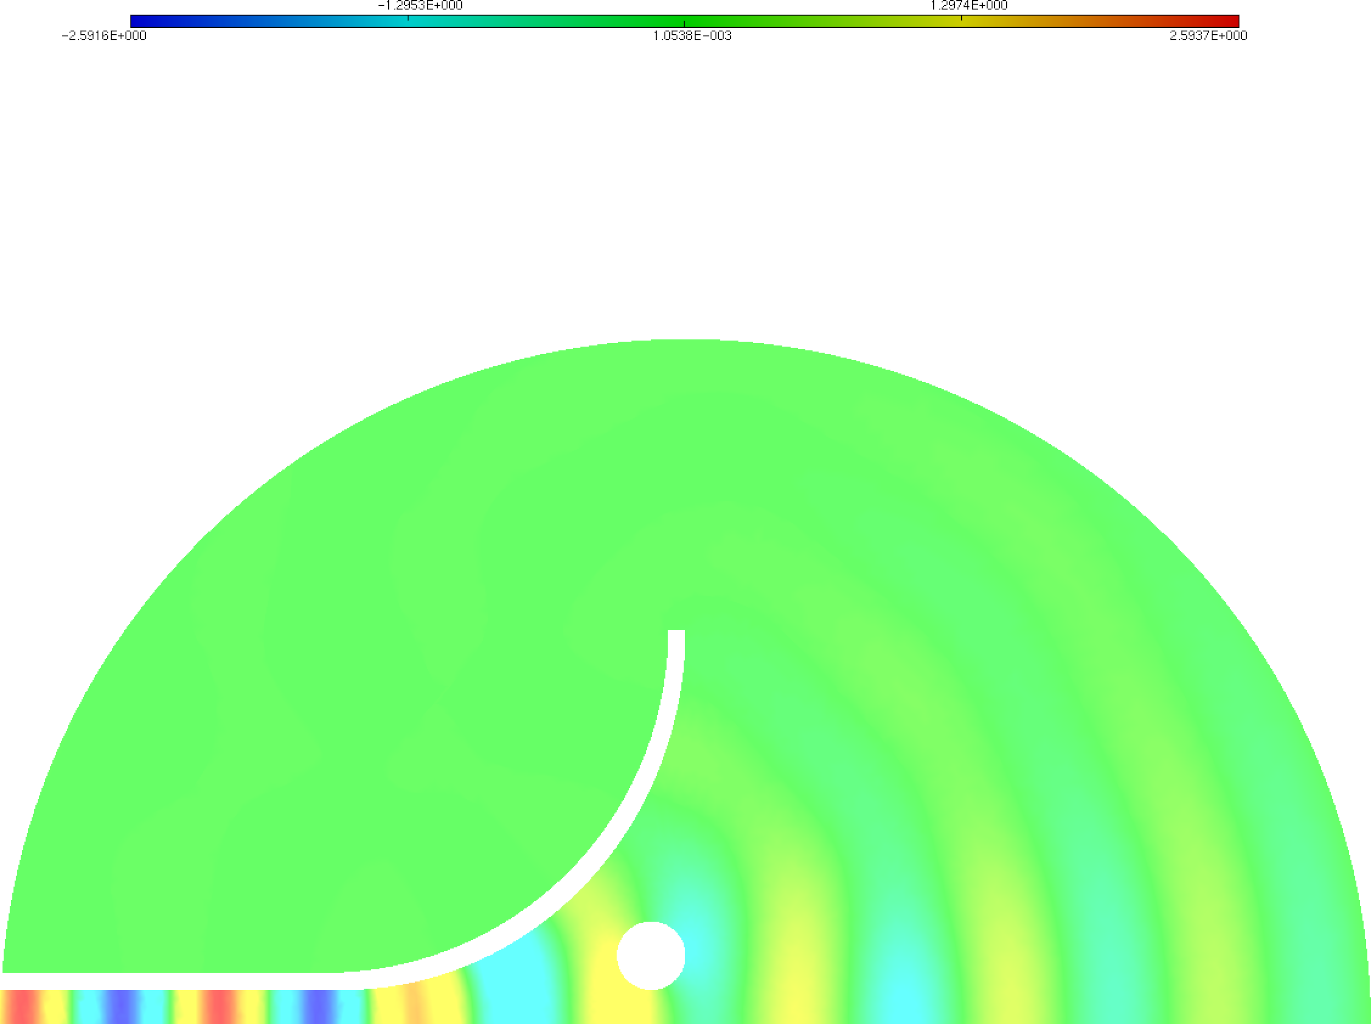
\includegraphics[width=0.45\textwidth]{figs/32}\hfill
\end{Verbatim}

\begin{itemize}
\item Since \verb!trunc! modifies \verb!T!, the finite element spaces that are defined on \verb!T! are also modified. Visualizing \verb!rho! just before and just after \verb!rho=1.0! shows that before, \verb!rho! is defined on the domain that contains the hole, while after, it gets redefined according to the updated finite element space \verb!V0!.  
\end{itemize}
%%%%%%%%%%%%%%%%%%%%%%%%%%%%%%%%%%%%%%%%%%%%%%%%%%%%%%%%%%%%%%%%%%%%%%%%%%%%%%%%

\textbf{4.4 Comparison of the results obtained in \S4.1 and \S4.2}
\begin{Verbatim}[commandchars=\\\{\}]
fespace V2OnOriginalMesh(originalMesh, P2);

// SET ZEROS WITHIN OBJECT FOR ORIGINAL MESH SOLUTION uOnTReal
V2OnOriginalMesh uTmp = uOnTReal * (region == air);
plot(uTmp, value = true, fill = true, nbiso = 64, wait = true);

// EXTEND WITH ZEROS uOnTtReal TO ORIGINAL MESH
int[int] rest = restrict(V2, V2OnOriginalMesh, n2o);
V2OnOriginalMesh uRealExtended;
for[i, j : rest] uRealExtended[][j] = uOnTtReal[][i];

// CHECK THE DIFFERENCE
V2OnOriginalMesh diff = abs(uRealExtended - uTmp);
real L2Norm = sqrt(int2d(originalMesh)(diff*diff));
cout << "USER/ The L2 norm of the difference is: " << L2Norm << endl;
plot(diff, value = true, fill = true, nbiso = 64, wait = true);
\dotfill
The L2 norm of the difference is: 3.65286e-09

\hfill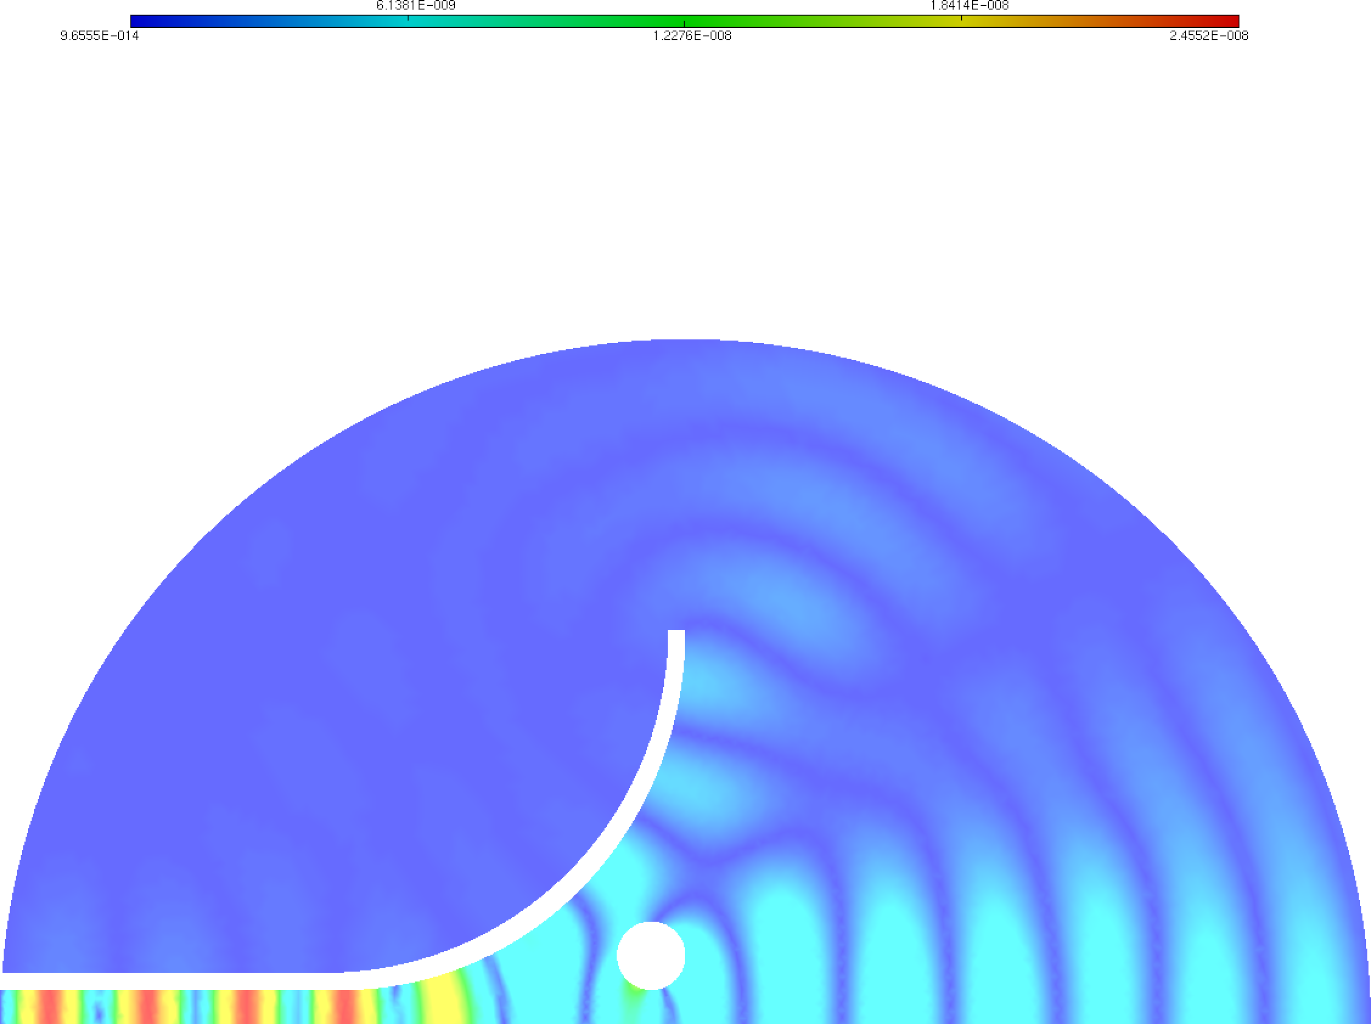
\includegraphics[width=0.45\textwidth]{figs/33}\hfill
\end{Verbatim}

\begin{itemize}
\item This snippet requires to store the original mesh, \verb!mesh originalMesh = T!, before calling \verb!trunc!.
\item First, the solution on the original mesh is set to vanish in $S$, since the comparison makes sense only in the physical parts of the domain. On the other hand, the solution on the truncated mesh is extended with zeros in $S$. Then, their difference is vanishing in $S$ by construction, and hence, the $L^2(\varOmega\setminus\overline{S})$ norm is essentially computed throughout the physical part of the domain.
\end{itemize}
%%%%%%%%%%%%%%%%%%%%%%%%%%%%%%%%%%%%%%%%%%%%%%%%%%%%%%%%%%%%%%%%%%%%%%%%%%%%%%%%

\textbf{4.5 A three-dimensional horn in parallel}
\begin{Verbatim}[commandchars=\\\{\}]     
macro dimension() 3        // 
macro partioner() parmetis // change partioner; default is metis
load "PETSc-complex"
include "macro_ddm.idp"
include "meditMPI.idp"
include "xmpl-09-geo.idp"

func Pk = P1;                       // keep element type consistent  
macro grad(u) [dx(u), dy(u), dz(u)] // define gradient

// BOUNDARIES AND INDICATORS ARE DEFINED IN xmpl-09-geo.idp
int n = 10;
mesh T = buildmesh(a001(16*n) + a002(16*n) + a003(4*n) +
                   a004(4*n)  + a005(n/5)  + a006(8*n) +
                   a007(4*n)  + a008(n)    + a009(-8*n));
mesh3 T3 = buildlayers(T, 40, zbound    = [0, -2.0*pi],
                              transfo   = [y*cos(z), x, y*sin(z)],
                              facemerge = true);
                              
// STORE ORIGINAL MESH AND INITIALIZE n2o FOR GLOBAL SOLUTION PLOT
mesh3 originalMesh = T3;
int[int] n2o;
macro T3N2O() n2o //

// DISTRIBUTE, DEFINE, ASSEMBLE, SOLVE
Mat<complex> A;   // define A as complex
createMat(T3, A, Pk);

real k = 2.0*pi*1200/345.0;
varf a(u, v) = int3d(T3)( grad(u)'*grad(v) )
             + int3d(T3)(-k*k*u*v )
             + int2d(T3, absorbBndLabel)( 1.0i*k*u*v + u*v )
             + int2d(T3, sourceBndLabel)( 1.0i*k*u*v );
varf l(u, v) = int2d(T3, sourceBndLabel)( 2.0i*k*v );
fespace V(T3, Pk);
A = a(V, V, tgv = -1);
set(A, sparams = "-ksp_type preonly -pc_type lu");
complex[int] b = l(0, V, tgv = -1); // define b as complex
V<complex> u;                       // define u as complex
u[] = A^-1*b;

// POSTPROCESSING 
V uReal = real(u);
medit("Local solutions", T3, uReal);
meditMPI(originalMesh, V, Pk, A, u, complex, n2o);
\dotfill

\hfill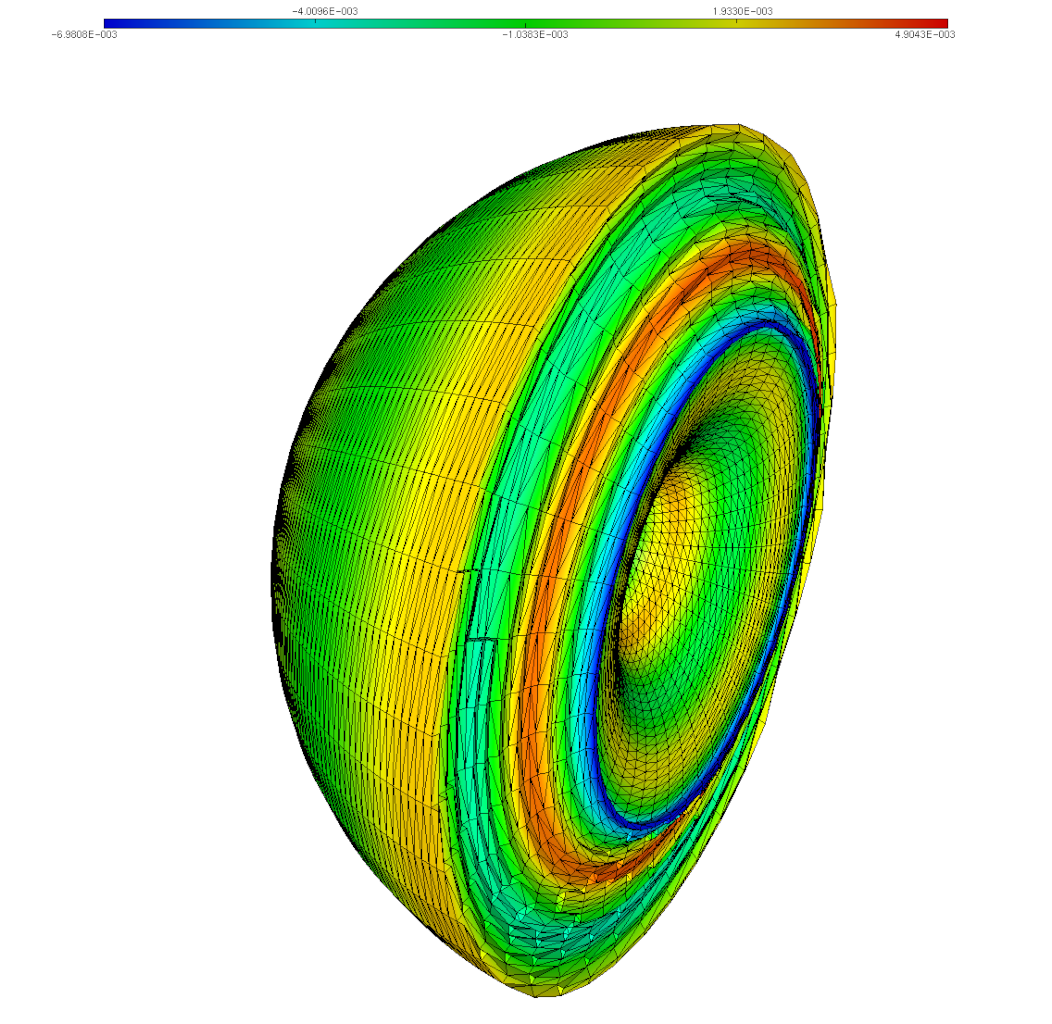
\includegraphics[width=0.45\textwidth]{figs/34}\hfill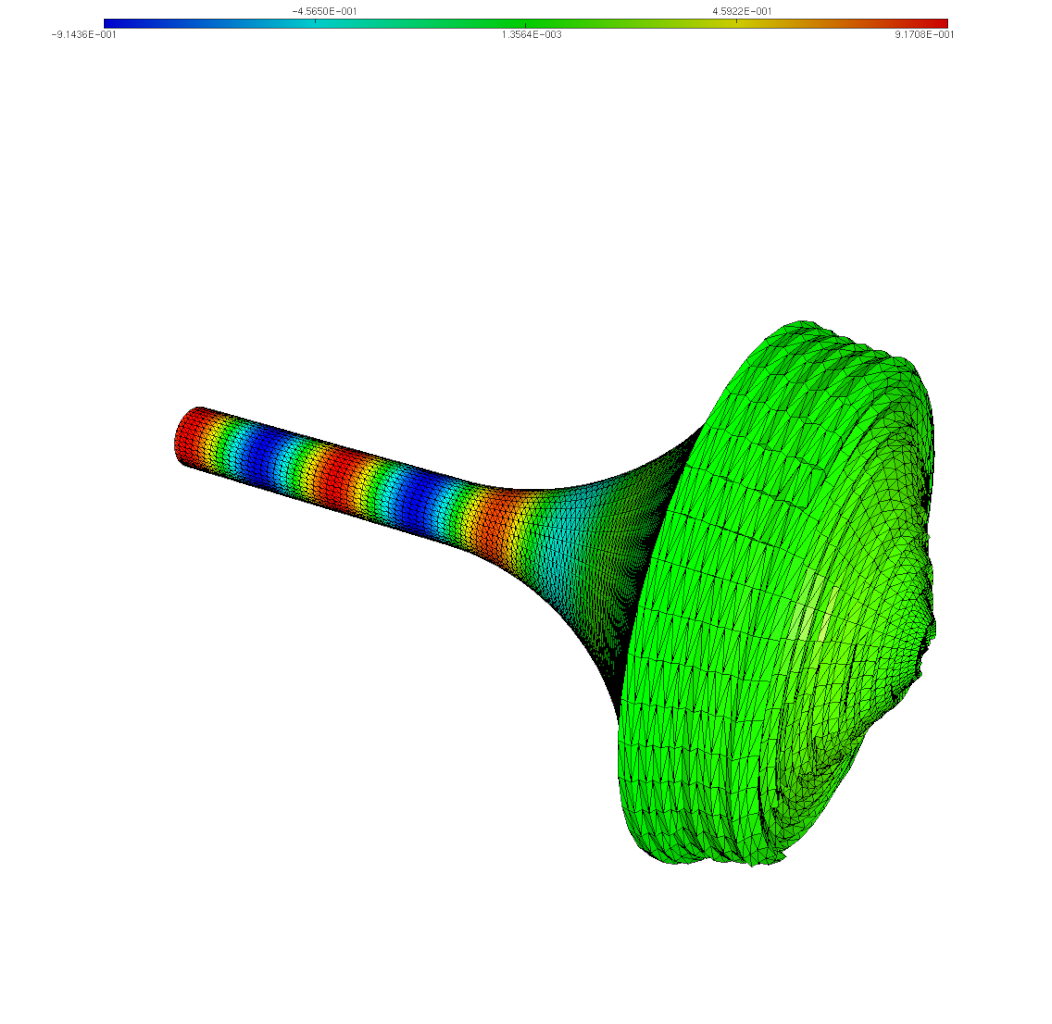
\includegraphics[width=0.45\textwidth]{figs/35}\hfill
\hfill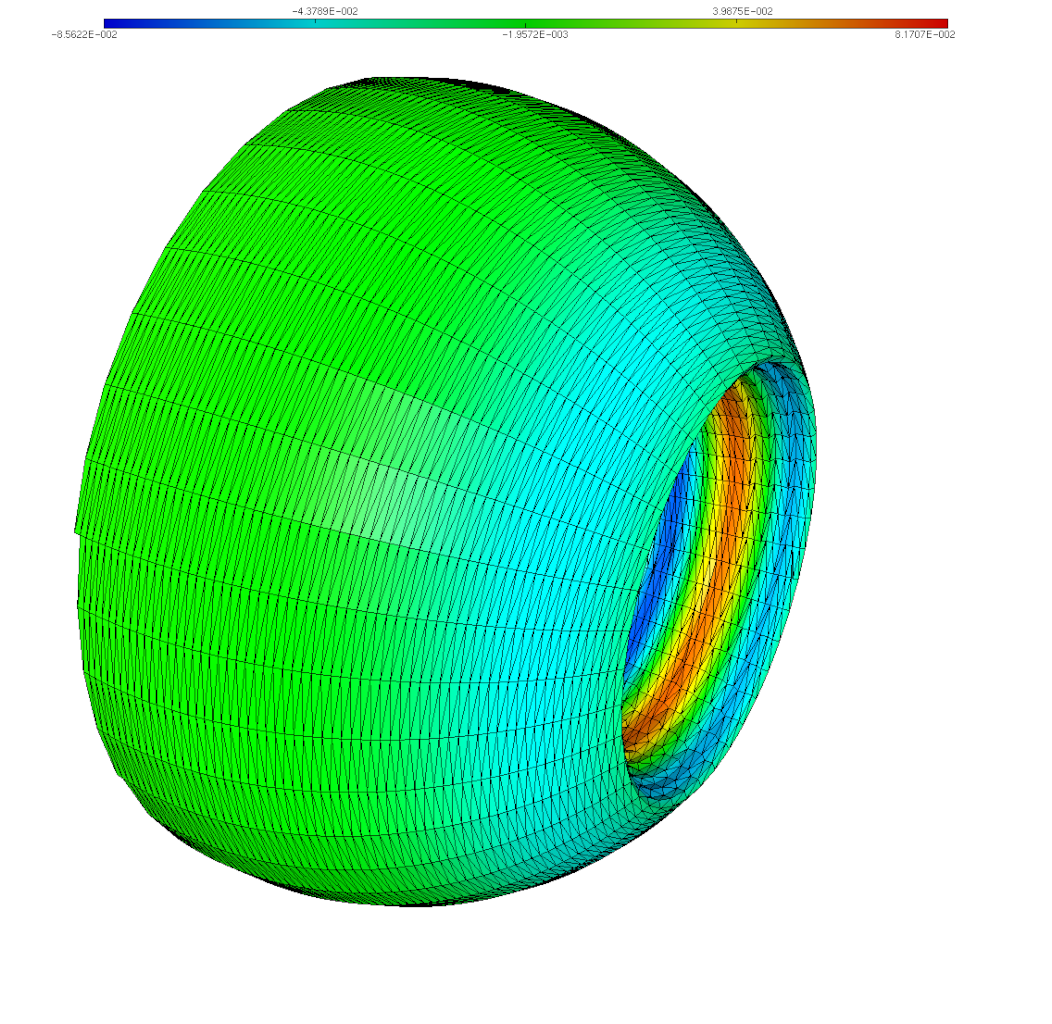
\includegraphics[width=0.45\textwidth]{figs/36}\hfill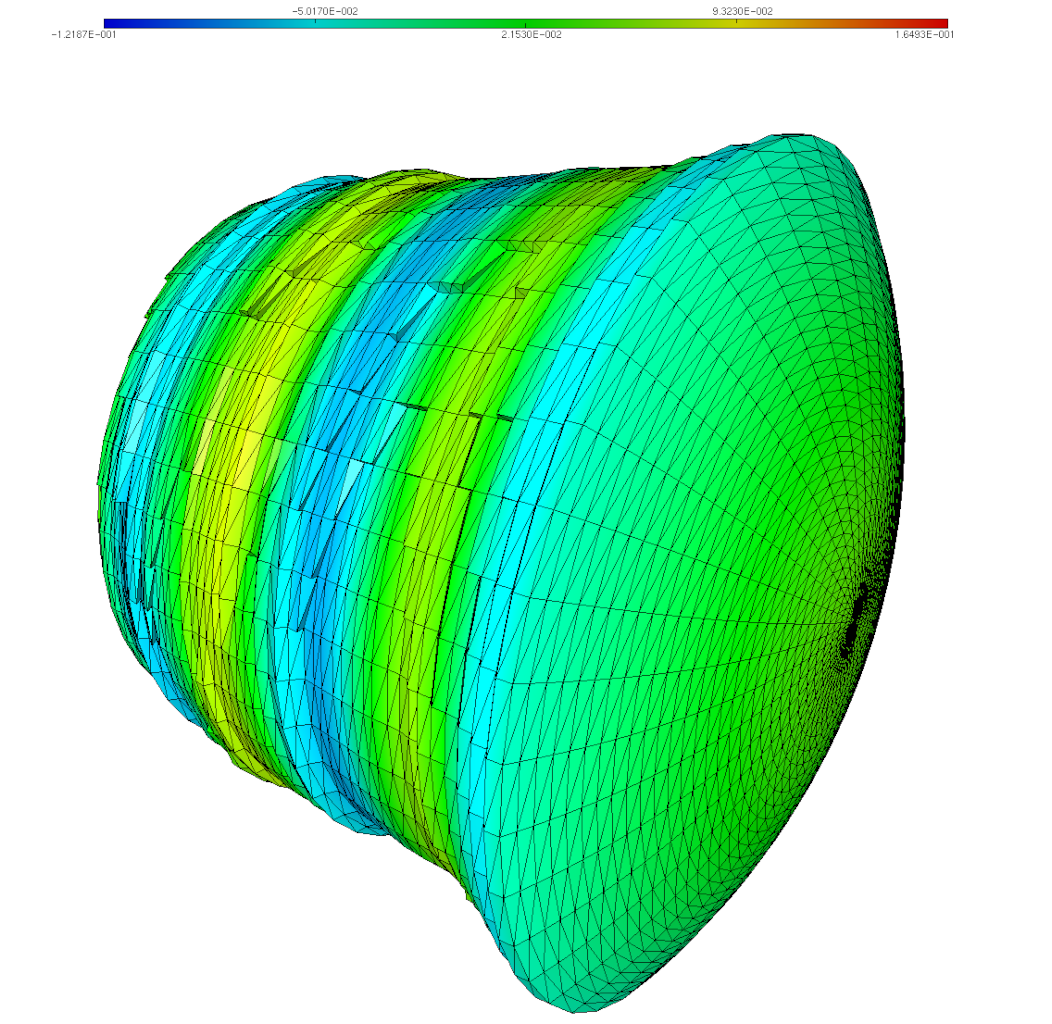
\includegraphics[width=0.45\textwidth]{figs/37}\hfill

\hfill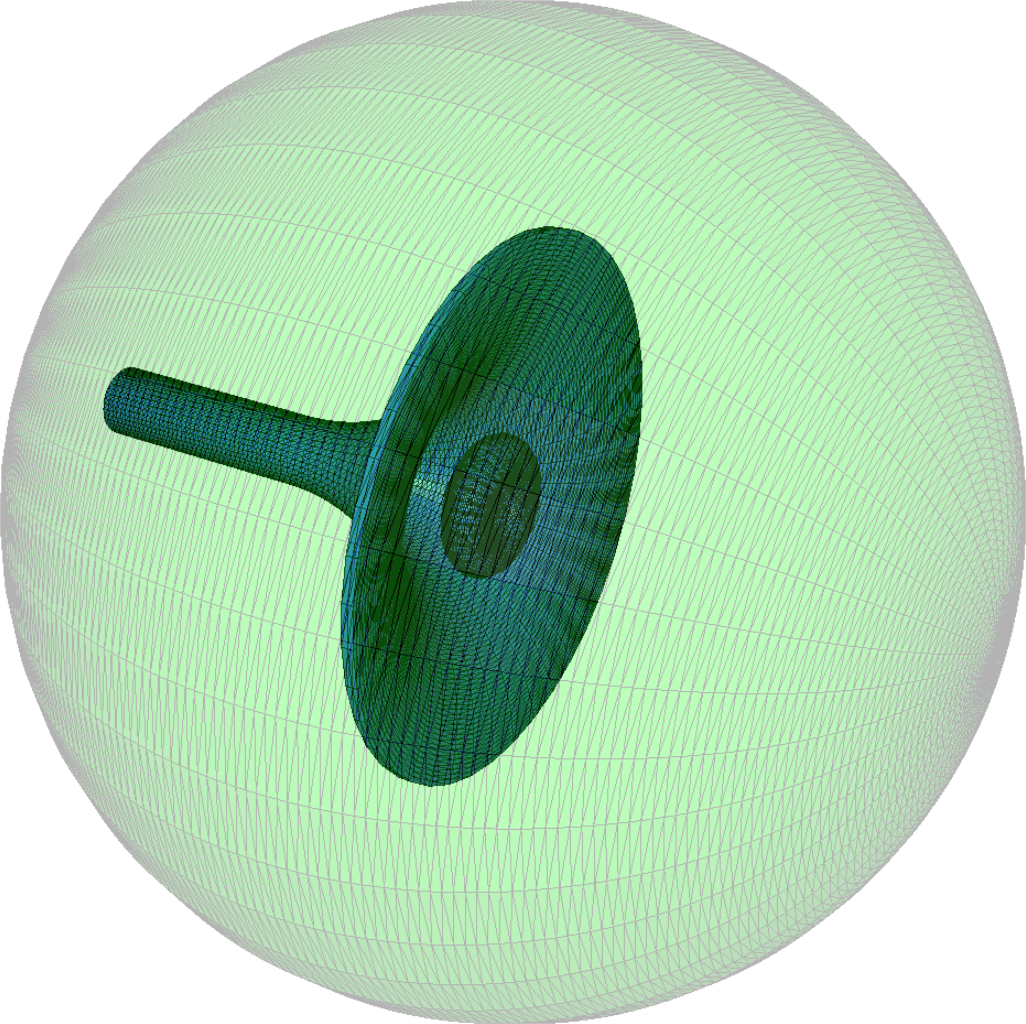
\includegraphics[width=0.38\textwidth]{figs/38}\hfill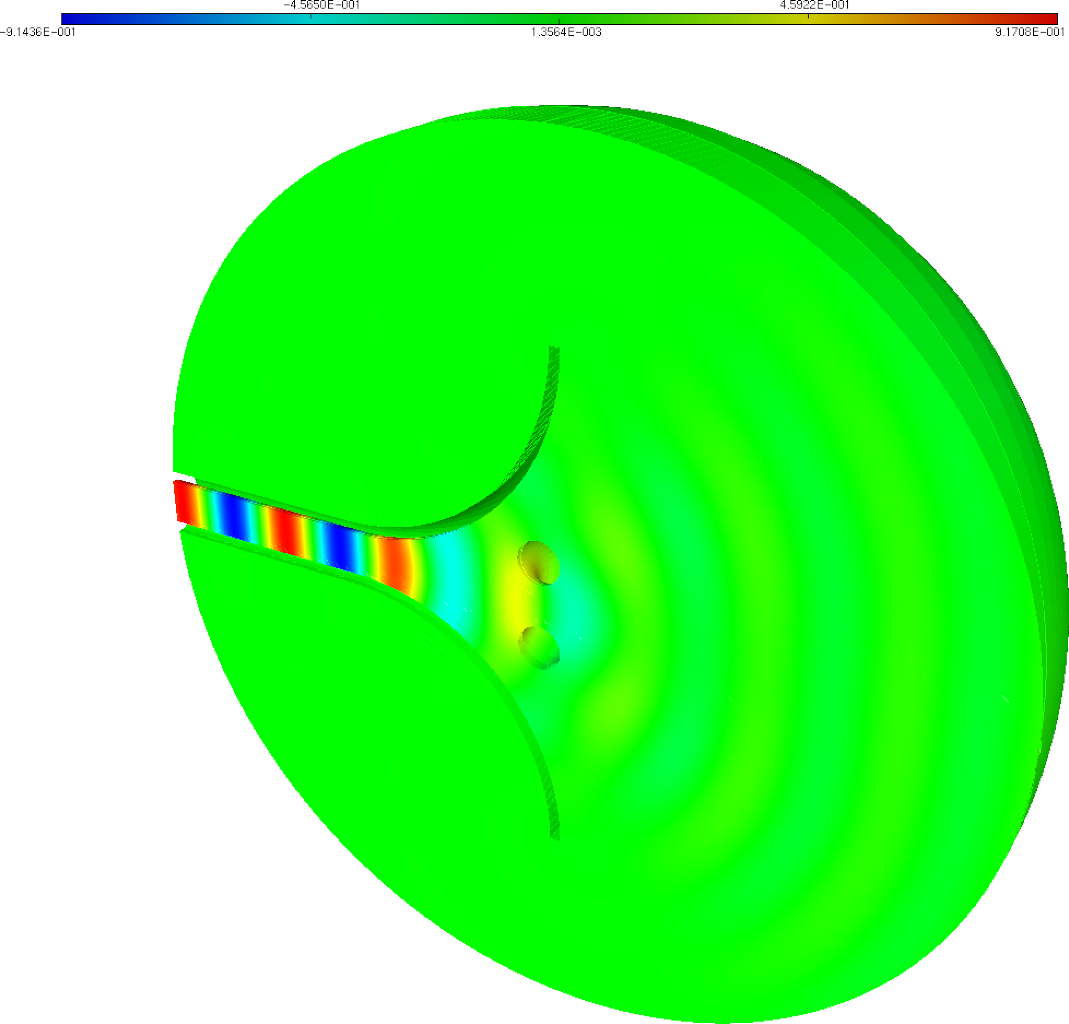
\includegraphics[width=0.45\textwidth]{figs/39}\hfill
\end{Verbatim}

\begin{itemize}
\item The file \verb!meditMPI.idp! includes \verb!medit! itself, while it defines a macro that performs the operations presented in the end of \S3.5 for collecting the local solutions to the zeroth process. It is not part of FreeFEM.
\item Since the finite element basis is consistently the same throughout the file, the type of elements is defined as a function \verb!func! without input arguments. In general, such \verb!func! objects can be functions of \verb!x!, \verb!y!, and \verb!z!, without explicitly defining the input arguments. Functions with input arguments can be defined according to the template \verb!func <dataType> funcName (<dataType> inName)!.
\item For \verb!real[int]! arrays \verb!a! and \verb!b!, the expression \verb!a'*b! returns the scalar product \verb!a[0]*b[0]+...+a[a.n-1]*b[b.n-1]!.
\item Since the problem is complex-valued, \verb!PETSc-complex! is loaded, instead of \verb!PETSc!, while \verb!Mat<complex>!, \verb!complex[int]!, and \verb!V<complex>! are used.
\end{itemize}

\section{\hrulefill\\Tutorial 5. Additional Mesh-Related Tools}
Two-dimensional meshing tools are explained in sufficient detail in the documentation of FreeFEM, with functions such as \verb!adaptmesh!, \verb!splitmesh!, \verb!trunc! being able to handle many occuring scenarios; a simple example is given below.

\vspace*{0.2cm}
\textbf{5.1 A two-dimensional adaptivity example}
\begin{Verbatim}[commandchars=\\\{\}]     
border a001(t = 0.0*pi, 1.0*pi)\{x = cos(t)  ; y = sin(t)  ;\}
border a002(t = 1.0*pi, 2.0*pi)\{x = cos(t)  ; y = sin(t)  ;\}
border a003(t = 0.0*pi, 2.0*pi)\{x = cos(t)/2; y = sin(t)/4;\}
mesh T = buildmesh( a001(25) + a002(100) + a003(300) );
plot(T, wait = true, cmm = "Original mesh");
real hmax = 0.1; // approximate maximum mesh size
int reg = T(0.0, 0.0).region;

// ADAPTMESH BASED ON REGION/LABEL FUNCTION
func f = hmax - 0.8*hmax*( region==reg ) - 0.8*hmax*( label==a001 );
T = adaptmesh(T, f, IsMetric = true, nbvx = 100000);
plot(T, wait = true, cmm = "Modified mesh");

// ADAPTMESH BASED ON LAPLACIAN FIELD
varf a(u, v) = int2d(T)( dx(u)*dx(v) + dy(u)*dy(v) )
             + on(a001, a002, a003, u = 0); // u value is not used
varf l(u, v) = on(a001, a002, u = hmax) + on(a003, u = 0.2*hmax);
fespace V1(T, P1);
V1 u;
matrix A = a(V1, V1, tgv = -1);
real[int] b = l(0, V1, tgv = -1);
u[] = A^-1*b;
T = adaptmesh(T, u, IsMetric = true, nbvx = 100000);
plot(T, wait = true, cmm = "New modified mesh");

// GET MAXIMUM SIDE-LENGTH OF EACH TRIANGLE
fespace V0(T, P0);
V0 hSize = hTriangle;
plot(hSize, value = true, fill = true, nbiso = 64, wait = true);
\dotfill

\hfill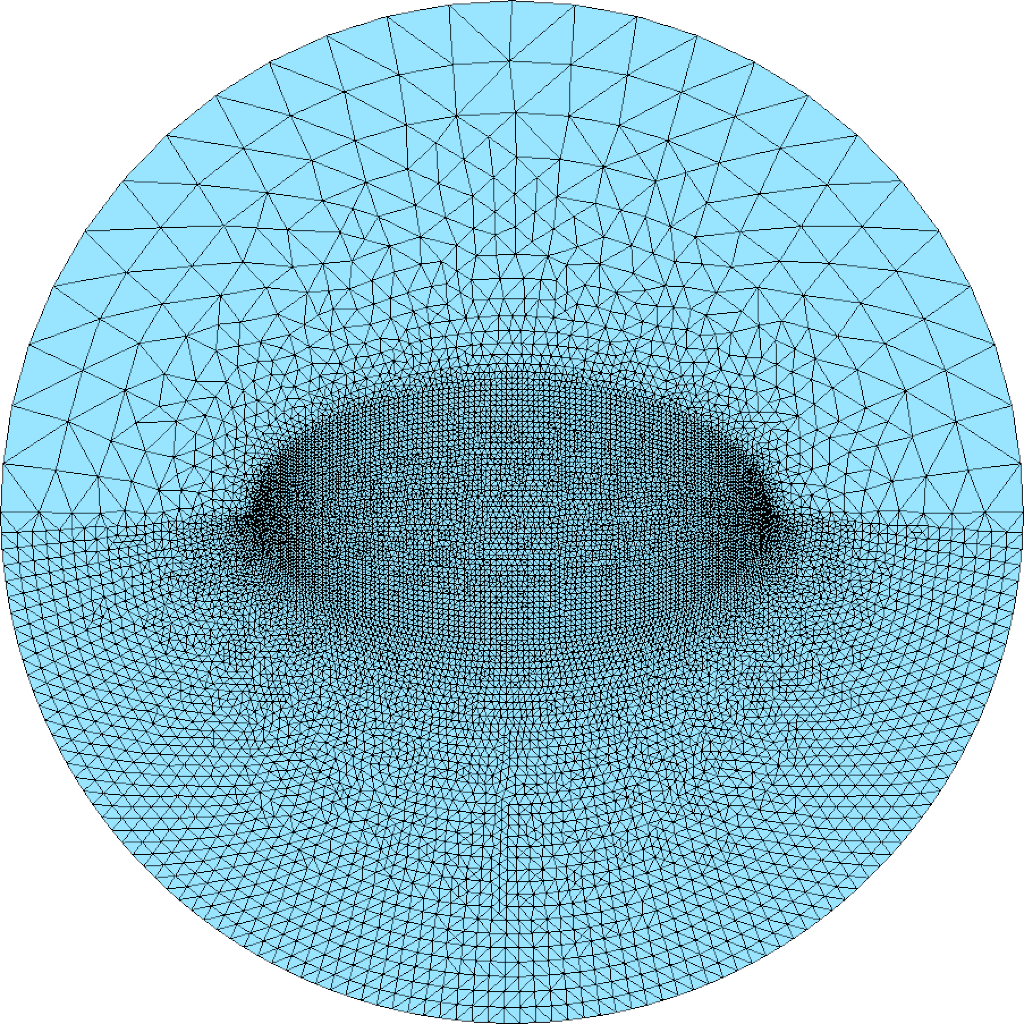
\includegraphics[width=0.4175\textwidth]{figs/40}\hfill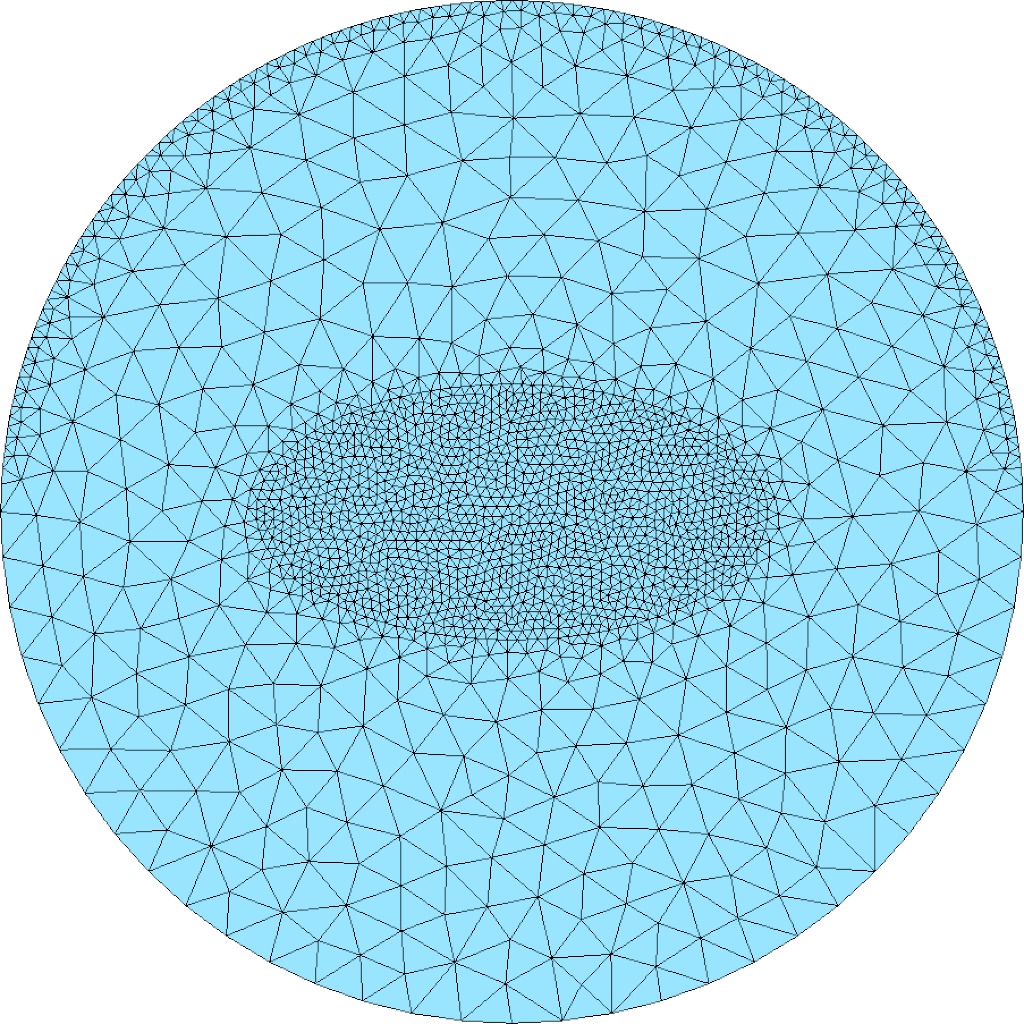
\includegraphics[width=0.4175\textwidth]{figs/41}\hfill

\hfill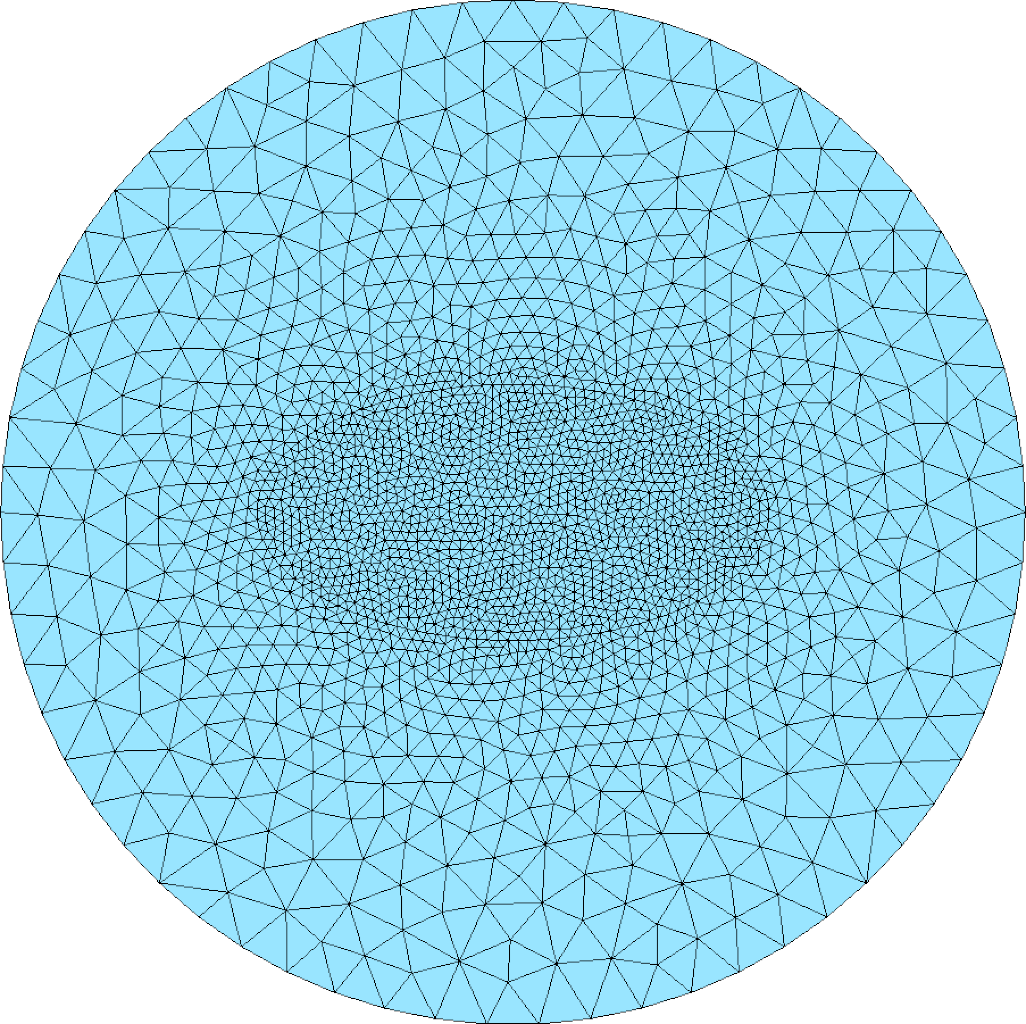
\includegraphics[width=0.4175\textwidth]{figs/42}\hfill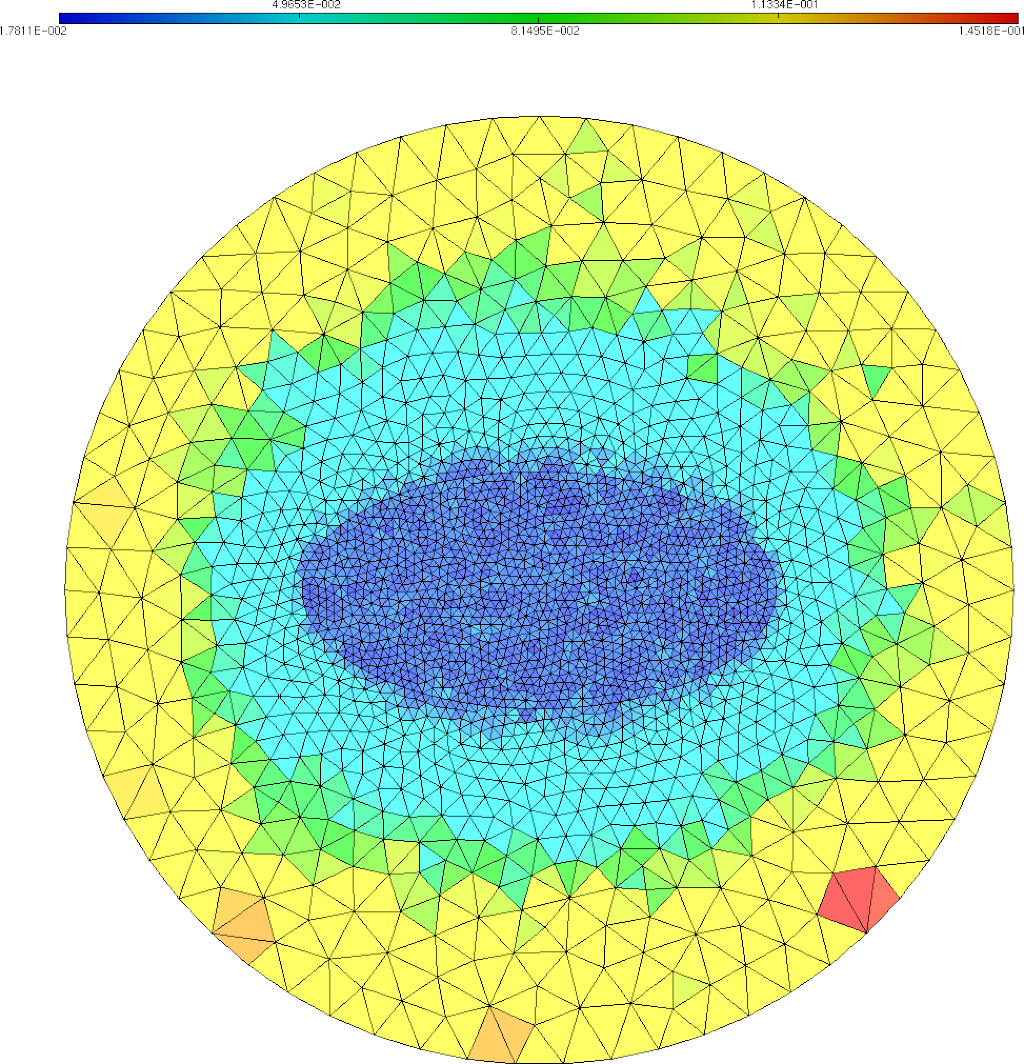
\includegraphics[width=0.45\textwidth]{figs/43}\hfill
\end{Verbatim}

\begin{itemize}
\item Refining the mesh in the vicinity of a border is particularly useful, when it is known that the solution varies rapidly close to that border, while refining the mesh with a Laplacian field is particularly useful, when the domain of interest is embedded into a space truncating domain, and hence, far from from the domain of interest, the density of elements does not need to be high.
\item Successive calls to \verb!adaptmesh! can result in triangulations that better meet the criteria provided by the defined fields, if so required.
\end{itemize}
%%%%%%%%%%%%%%%%%%%%%%%%%%%%%%%%%%%%%%%%%%%%%%%%%%%%%%%%%%%%%%%%%%%%%%%%%%%%%%%%

\vspace*{0.2cm}
\textbf{5.2 Three-dimensional meshing}\\
The geometry of interest is a coil within a bounding box. The default number of windings is set to unity, while the user can set a different number of windings by calling FreeFEM with the option \verb!-now! followed by the desired number of windings, which provides a value for the \verb!nOfWindings! variable through the \verb!getARGV! function.
\begin{Verbatim}[commandchars=\\\{\}]
// TWO-DIMENSIONAL MESH
border a001(t = 0, 2.0*pi) \{
  x = R + r*cos(t); y = r*sin(t); label = 0; \}
int resMesh2D = 25; // two-dimensional mesh resolution
mesh T2 = buildmesh( a001(resMesh2D) );

int surfIndicator = T2(R, 0.0).region;

// GENERATE THREE-DIMENSIONAL MESHES OF INTERIOR OBJECTS
int[int] labTo0 = [surfIndicator, 0]; // [old, new]
int[int] labTo1 = [surfIndicator, 1];
int[int] labTo2 = [surfIndicator, 2];
mesh3 T3Coil = buildlayers(T2, nOfWindings*200,
                        zbound    = [2.0*pi*nOfWindings, 0.0],
                        transfo   = [x*cos(z), x*sin(z), w*z + y],
                        labelup   = labTo0,
                        labeldown = labTo0); // coil

mesh3 T3PipeL = buildlayers(T2,  75, zbound = [0.0, -3.0*R],
                        transfo   = [x, z, y],
                        labelup   = labTo1,
                        labeldown = labTo0); // lower pipe

mesh3 T3PipeU = buildlayers(T2,  75, zbound = [3.0*R, 0.0],
                        transfo   = [x, z, 2*pi*nOfWindings*w + y],
                        labelup   = labTo0,
                        labeldown = labTo2); // upper pipe
\end{Verbatim}

\begin{itemize}
\item Start by defining a \verb!mesh! triangulation \verb!T2! for the disk of radius \verb!r! whose center is located at \verb!(R,0)!. The boundary of that disk is labeled zero, while its domain indicator is stored in the variable \verb!surfIndicator!. In some sense, these tags are preserved by \verb!buildlayers!.
\item In particular, when calling \verb!buildlayers!, the surface that is formed by repetitions of the boundary of the disk is prescribed the label of that boundary, \verb!labelmid!, while the surfaces that are formed by the disk are assigned the domain indicator that is associated with the disk surface, \verb!labelup! and \verb!labeldown!.
\item Here, the indicator \verb!0! is used for coil surfaces on which no boundary conditions are imposed. Hence, for each pipe that is attached to the body of the coil, the default indicator \verb!0! of the disk boundary is kept for the middle surface, the surface that is internal to the device is also assigned the indicator \verb!0!, while the surface that is exposed to the void domain is assigned a new identifier; here, \verb!1! and \verb!2! for the lower and upper pipe, respectively.
\end{itemize}

\begin{Verbatim}[commandchars=\\\{\}]
// OBTAIN THE SURFACE MESHES
T3Coil  = buildBdMesh(T3Coil ); // attach surface mesh to mesh3 objects
T3PipeL = buildBdMesh(T3PipeL);
T3PipeU = buildBdMesh(T3PipeU);
meshS T3CoilS  = T3Coil .Gamma; // extract surface meshes as meshS
meshS T3PipeLS = T3PipeL.Gamma;
meshS T3PipeUS = T3PipeU.Gamma;

// BOUNDING BOX SURFACE MESH / NEEDS MeshSurface.idp
int[int]       boxRes = [50, 50, 50];
real[int, int] boxLim = [[-4.0*R, 4.0*R], [-4.0*R, 4.0*R],
                         [-3*R, 2*pi*nOfWindings*w + 3.0*R]];
int [int, int] boxLab = [[3, 3], [3, 3], [3, 3]];
meshS T3BoxS = SurfaceHex(boxRes, boxLim, boxLab, -1);

// GLUE SURFACE MESHES
meshS T3AllS = T3BoxS + T3CoilS + T3PipeLS + T3PipeUS;

// BUILD THREE-DIMENSIONAL MESH WITH TETGEN
mesh3 T3 = tetg(T3AllS, switch = "pqAQ");
medit("First mesh", T3);

// SET TWO DOMAIN INDICATORS
int coil = 1, void = 2;
int[int] regIndicators = regions(T3);
T3 = change(T3, fregion = coil*(region == regIndicators[0]) +
                          void*(region == regIndicators[1]) +
                          coil*(region == regIndicators[2]) +
                          coil*(region == regIndicators[3]));

// THREE-DIMENSIONAL MESH REFINEMENT
fespace V1(T3, P1);
V1 iso = 0.05*( region == coil ) + 0.5*( region == void ); // mesh size
T3 = mmg3d(T3, metric = iso[]);
medit("Final mesh", T3);
\end{Verbatim}

\begin{itemize}
\item For each volume mesh that is generated with \verb!buildlayers!, the surface mesh \verb!meshS! is extracted with the \verb!.Gamma! method, after a call to \verb!builBdMesh!. The surface mesh of the bounding box is generated with the function \verb!SurfaceHex!, and the four surface meshes are glued together.
\item Although it is possible to pass a particular volume indicator for each one of the four domains, here, since the number of domains is small, the call to \verb!tetg! is kept minimal, and domain indicators are assigned afterwards, with the function \verb!change!.
\item Finally, Mmg is used for setting the characteristic mesh length in the coil and in the void domains.
\end{itemize}

\begin{Verbatim}[commandchars=\\\{\}]
> FreeFem++ xmpl-12.edp -now 5
\dotfill

\hfill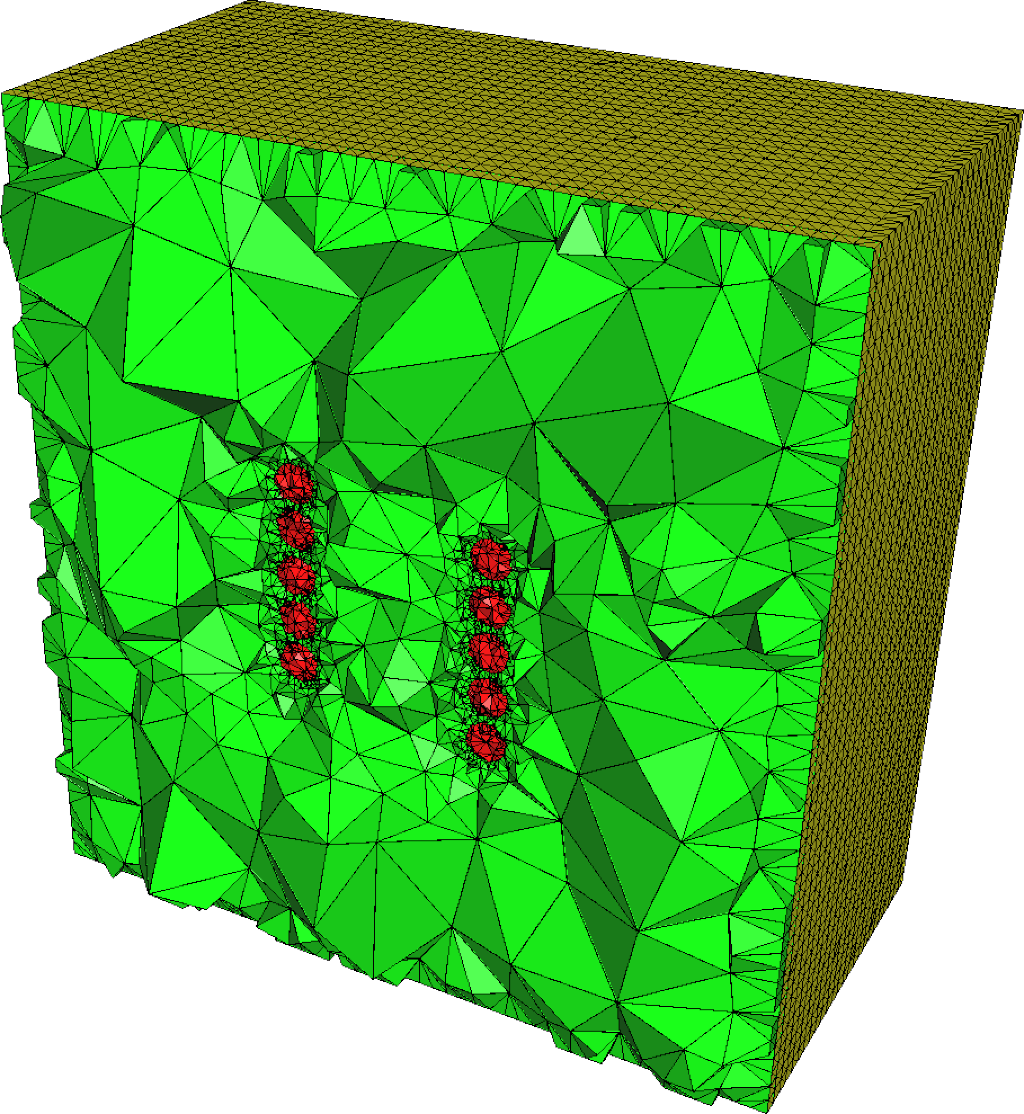
\includegraphics[width=0.45\textwidth]{figs/44}\hfill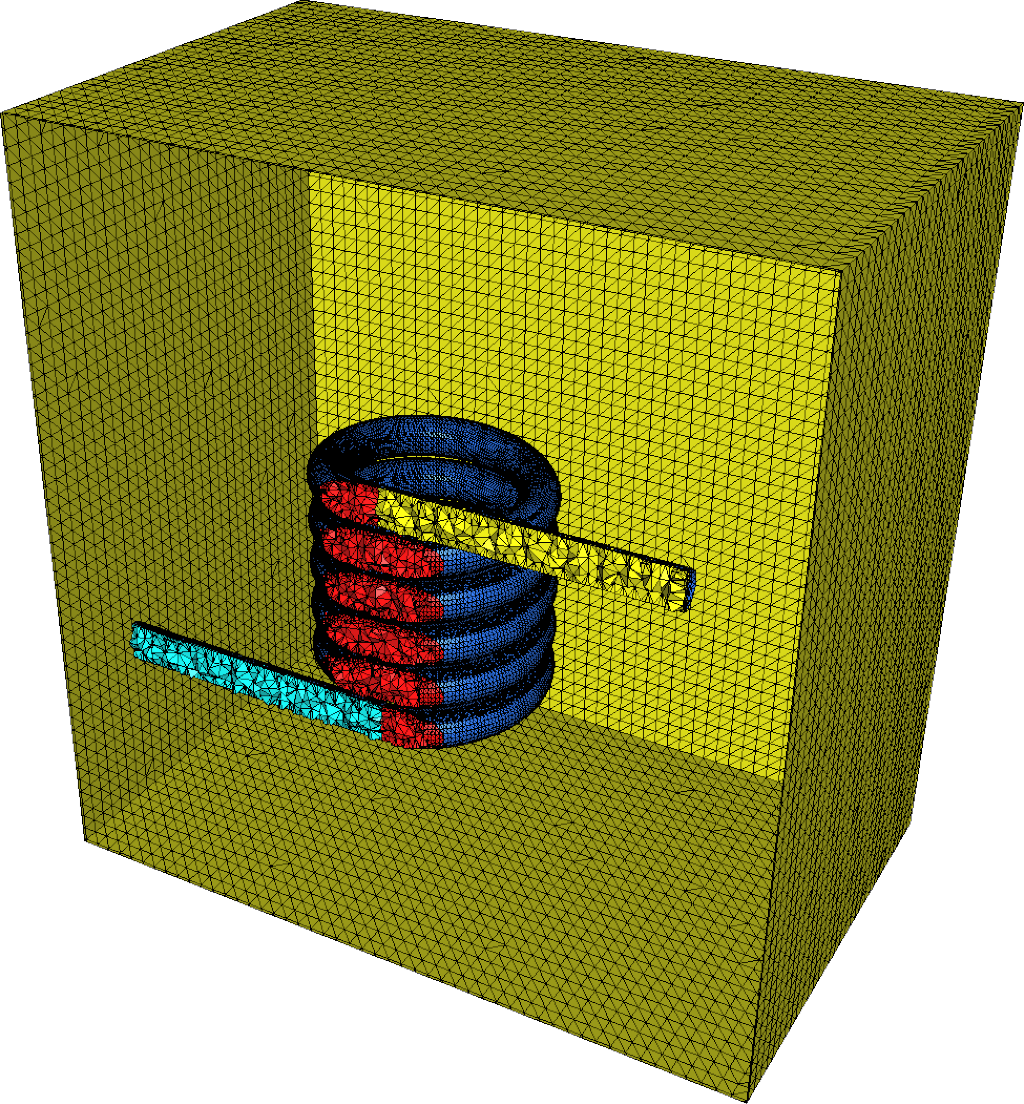
\includegraphics[width=0.45\textwidth]{figs/45}\hfill

\hfill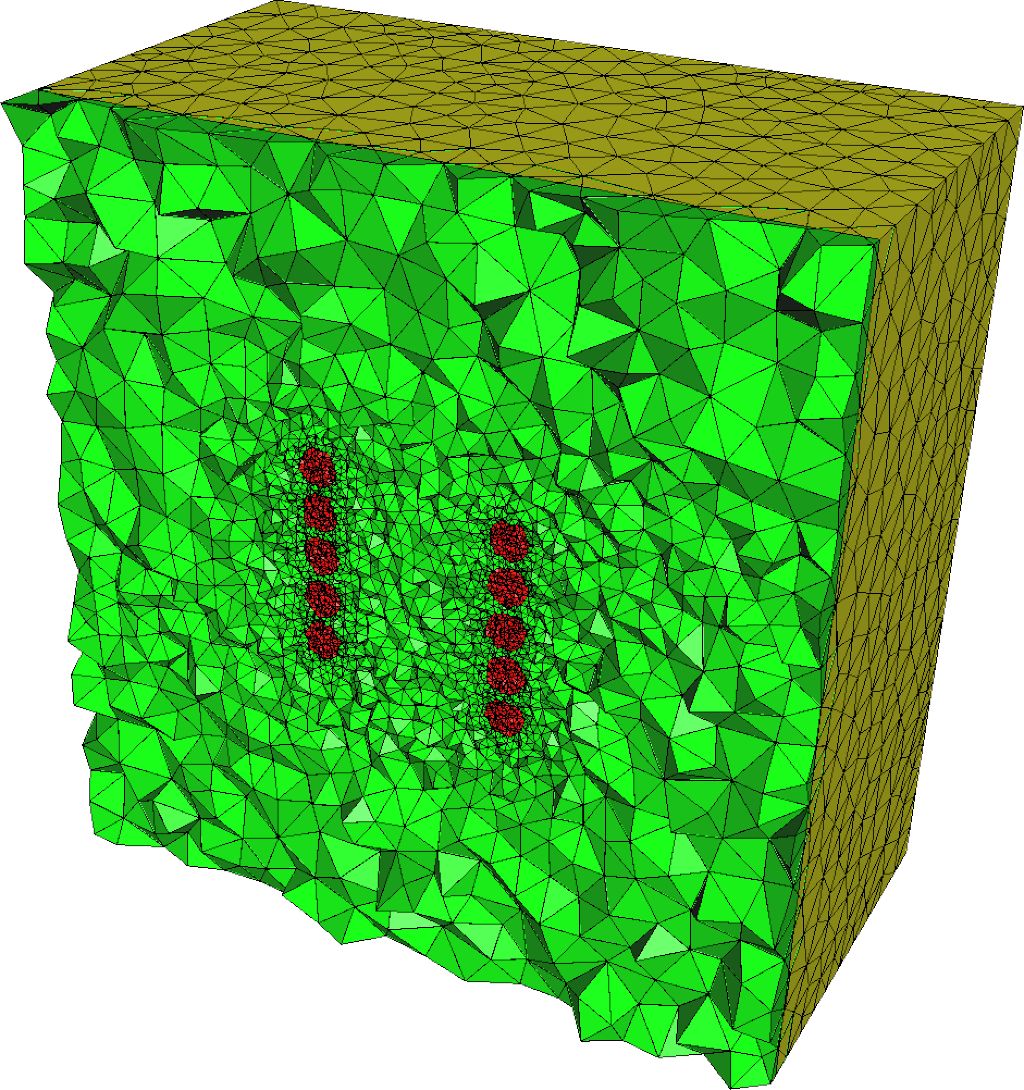
\includegraphics[width=0.45\textwidth]{figs/46}\hfill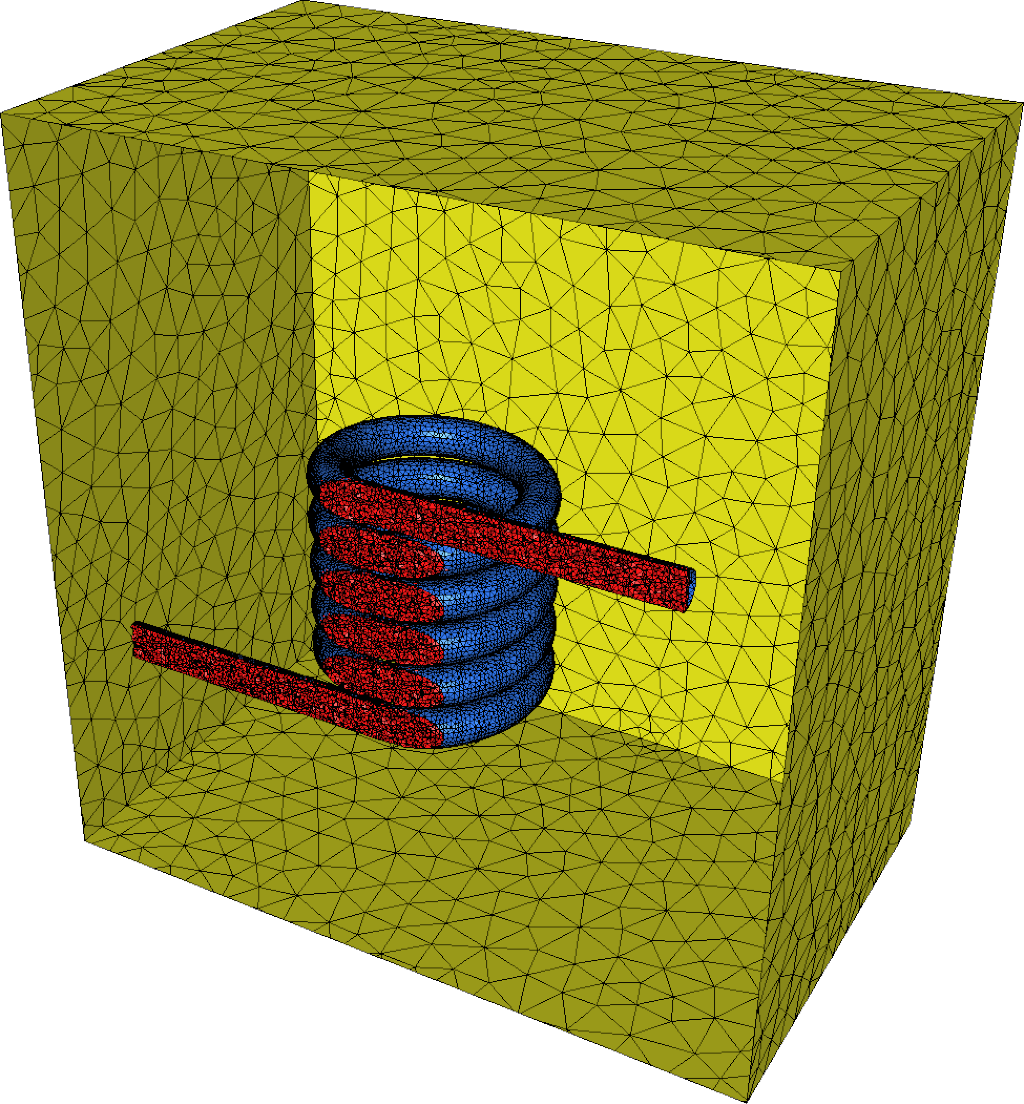
\includegraphics[width=0.45\textwidth]{figs/47}\hfill
\end{Verbatim}

\section{\hrulefill\\Appendix. A Note on PETSc Solvers and Preconditioners}
Let $m>1$ be an integer, $\bm{A}\in\mathbb{R}^{m\times m}$ a non-singular matrix, and $\bm{b}\in\mathbb{R}^m$. Provided an initial guess $\bm{u}_0\in\mathbb{R}^m$, Krylov space methods for solving $\bm{Au}=\bm{b}$ generate a sequence of improving approximations $\bm{u}_n$ such that
\[
\bm{u}_n - \bm{u}_0\in\operatorname{span}(\bm{r}_0,\bm{Ar}_0,\ldots,\bm{A}^{n-1}\bm{r}_0)\equiv\mathcal{K}^n(\bm{A},\bm{r}_0),
\]
where $\bm{r}_n=\bm{b}-\bm{A}\bm{u}_n$, with $n\in\mathbb{N}$, is the residual in the $n$-th iteration, while $\mathcal{K}^n(\bm{A},\bm{r}_0)$ is called the Krylov space that is generated by the pair $(\bm{A},\bm{r}_0)$. Hence, in each iteration, Krylov space methods provide the approximation
\[
\bm{u}_n = \bm{u}_0 + p_n(\bm{A})\bm{r}_0,\quad\text{with }p_n(\bm{A})=\sum_{k=0}^{n-1}\alpha_k\bm{A}^k,
\]
for some scalars $\alpha_0,\ldots,\alpha_{n-1}$. To specify these scalars, each Krylov space method employs particular optimality constraints, depending on properties such as the symmetry and positive definiteness of $\bm{A}$. For instance, in each iteration, the conjugate gradient method minimizes the error $\Vert\bm{u}-\bm{u}_n\Vert_{\bm{A}}=(\bm{u}-\bm{u}_n)^\top\bm{A}(\bm{u}-\bm{u}_n)$ over the appropriate Krylov space, provided that $\bm{A}$ is symmetric and positive definite. In general, if $\bm{A}$ is symmetric and positive definite, then the conjugate gradient (CG) method, \verb!-ksp_type cg! in \verb!sparams! for PETSc, is the method of choice, while if $\bm{A}$ is symmetric and indefinite, the minimum residual (MINRES) method, \verb!-ksp_type minres!, can be used. For nonsymmetric matrices, the generalized minimum residual (GMRES) method is often employed. For a detailed exposition on Krylov space methods consult Y. Saad, Iterative methods for sparse linear systems, SIAM, 2003. The convergence properties of Krylov space methods depend on the spectral properties of the coefficient matrix $\bm{A}$ -- in general, a Krylov space method converges faster when the eigenvalues of $\bm{A}$ are clustered -- and hence, it is most often favorable to solve an equivalent linear system whose coefficient matrix exhibits improved spectral properties. In theory, and far from implementation, a (left) preconditioner can be viewed as an invertible matrix $\bm{P}\in\mathbb{R}^{m\times m}$ that turns the original system into the equivalent system $\bm{P}^{-1}\bm{A}\bm{u}=\bm{P}^{-1}\bm{b}$, with $\bm{P}^{-1}$ being close to the inverse of $\bm{A}$, in some sense, while being relatively easy to compute. Additional aspects such as symmetry preservation, the so-called fill-in effect (vanishing entries change to non-zero values, after applying a preconditioner, and the resulting matrix becomes less sparse), and the block structure of $\bm{A}$ have to be considered in practical implementations of preconditioners. Among others, diagonal scaling, incomplete factorizations, multilevel strategies, and domain decomposition methods serve as preconditioning approaches, and are available through \verb!-pc_type jacobi/ilu/icc/mg/gamg/hpddm!, respectively. For more information study the examples in \verb!https://doc.freefem.org/documentation/petsc/index.html!
\end{document}
